\frame{\frametitle{Variando la helicidad cruzada: Campos de Els\"asser}
  Las ecuaciones MHD en función de los campos de Els\"asser:
  \begin{equation*}\label{eq:ElsasserFields}
    \vec{z}^\pm = \vec{v} \pm \vec{b}
  \end{equation*}
  \begin{equation*}\label{eq:NS-Elsasser}
    \partial_t \vec{z}^\pm  = \pm  \vec{V_A} \cdot \nabla \vec{z}^\pm  - 
    \vec{z}^\mp \cdot \nabla \vec{z}^\pm - \nabla{P} + 
    \frac{1}{R} \nabla^2 \vec{z}^\pm
  \end{equation*}

  \begin{itemize}
    \item Asumimos: $P = p/\rho$ y $R = R_m$
  \end{itemize}
  \pause\vspace{10pt}
  \begin{columns}
    \column{0.8\textwidth}
    \begin{minipage}[t]{1\textwidth}
      \begin{center} 
  Invariantes ideales de MHD incompresible:
  \begin{equation*}
    E = \frac{1}{2}\int{\left(\left|\vec{v}\right|^2 +
      \left|\vec{b}\right|^2 \right)\,dV} =
    \frac{1}{4}\int{\left(\left|\vec{z}^+\right|^2 +
      \left|\vec{z}^-\right|^2 \right)\,dV}
  \end{equation*}
  \begin{equation*}
    H_c = \int{\vec{v}\cdot\vec{b} \, dV} =
    \frac{1}{4}\int{\left(\left|\vec{z}^+\right|^2 
    - \left|\vec{z}^-\right|^2 \right)\,dV}
  \end{equation*}
      \end{center}
    \end{minipage}
    \column{0.2\textwidth}
    \begin{minipage}[t]{1\textwidth}
      \begin{center}
        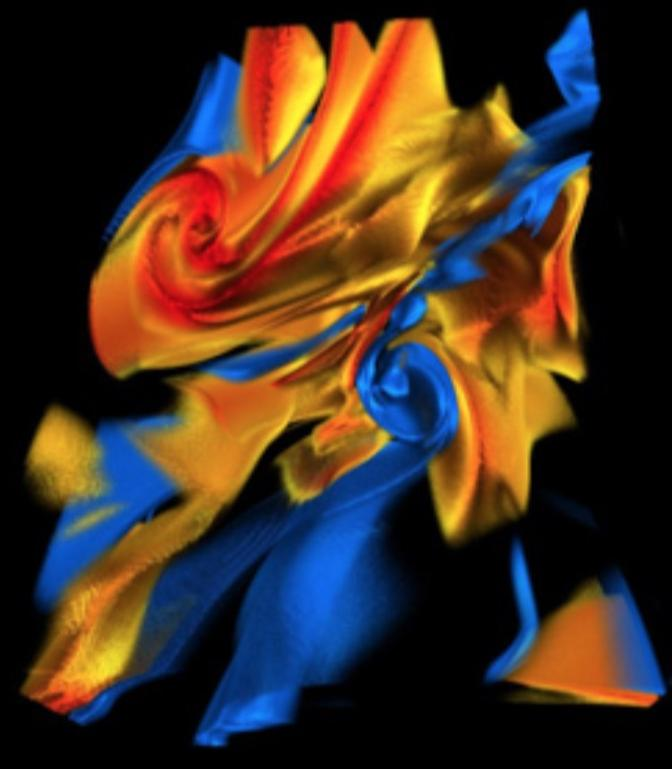
\includegraphics[width=\columnwidth]{extra/helicidad1.jpg}
      \end{center}
    \end{minipage}
  \end{columns}

}
\note[itemize]{
\item Para estudiar teniendo en cuenta el sentido de las propagaciónes, variables de Elsässer. Ahora el sentido de las propagaciones nos importa.
  \item Campos de las perturbaciones.
  \item Miembro derecho: térmico convectivo separado en parte lineal
    (propagación Alfvénica con $\vec{V_A}=\vec{B_0}$) y parte no
    lineal (interacción de fluctuaciones contrapropagantes).
  \item La helicidad cruzada es de relevancia para el viento solar y
    para los plasmas espaciales, pues los flujos de gran escala con
    helicidad cruzada se encuentran usualmente en el medio
    interplanetario.
}



\frame{\frametitle{Campos de Els\"asser}
  \begin{equation*}
    H_c = \int{\vec{v}\cdot\vec{b} \, dV} =
    \frac{1}{4}\int{\left(\left|\vec{z}^+\right|^2 
    - \left|\vec{z}^-\right|^2 \right)\,dV}
  \end{equation*}
  Podemos definir la helicidad cruzada normalizada:
  \begin{equation*}
    \sigma_c = H_c/E
  \end{equation*}
  \vspace{-20pt}
  \begin{itemize}
    \item $\sigma_c$ mide la cantidad de fluctuaciones
      contrapropagantes en el sistema.
    \item $\sigma_c = \pm 1$ corresponde a un único tipo de
      fluctuaciones $\vec{z}^\pm$, mientras $\sigma_c=0$ representa
      equipartición entre ambos campos.
    \item El estudio espacio-temporal de las variables de Els\"asser
      nos permitirá separar las dos posibles polarizaciones de las
      ondas de Alfvén, así como también las direcciones de
      propagación, y cuantificar cualquier desbalance entre ellas.
  \end{itemize}
}
\note[itemize]{
  \item
  \item SIMULACIONES
}




\frame{\frametitle{Simulaciones realizadas}
  \begin{table}
    \centering
    \begin{tabular}{|l||c||c||c||c||c||c|}
      \hline
      & $B_0=0$ & $B_0 = 0.25$ & $B_0 = 1$ & $B_0 = 2$ & $B_0 = 4$ & $B_0 = 8$ \\ \hline\hline
      & $0$ & $0$ & $0$ & $0$ & $0$ & $0$ \\ \cline{2-7} 
      $\sigma_c \approx $ & $0.3$ & $0.3$ & $0.3$ & $0.3$ & $0.3$ & $0.3$ \\ \cline{2-7} 
      & $0.9$ & $0.9$ & $0.9$ & $0.9$ & $0.9$ & $0.9$ \\ \hline
    \end{tabular}
    %\caption{Lista de simulaciones numéricas realizadas, con un campo guía
    %  $\vec{B} = B_0 \hat{x}$ y helicidad cruzada normalizada $\sigma_c$.}
    \label{tab:listSim}
  \end{table}
  \begin{itemize}
    \item Correlaciones entre los forzados mecánico y magnético para
      cambiar el nivel de helicidad cruzada en el flujo.
    \item Los $\sigma_c$ corresponden al promedio temporal en el estado
      turbulento estacionario.
    \item Todas las simulaciones fueron realizadas hasta que el
      sistema alcanzase un estado turbulento estacionario.
  \end{itemize}
}
\note[itemize]{
  \item Cada simulación tiene una helicidad cruzada instantánea que
    fluctúa en el tiempo alrededor de los valores medios reportados.
}







\frame{\frametitle{Espectros de energía y escalas de tiempo dominantes}
  Los espectros energéticos perpendiculares reducidos y los
  isocontornos del espectro axisimétrico de energía son similares a
  los ya obtenidos.
  \begin{columns}
    \column{0.4\textwidth}
    \begin{minipage}[t]{1\textwidth}
      \begin{center} 
        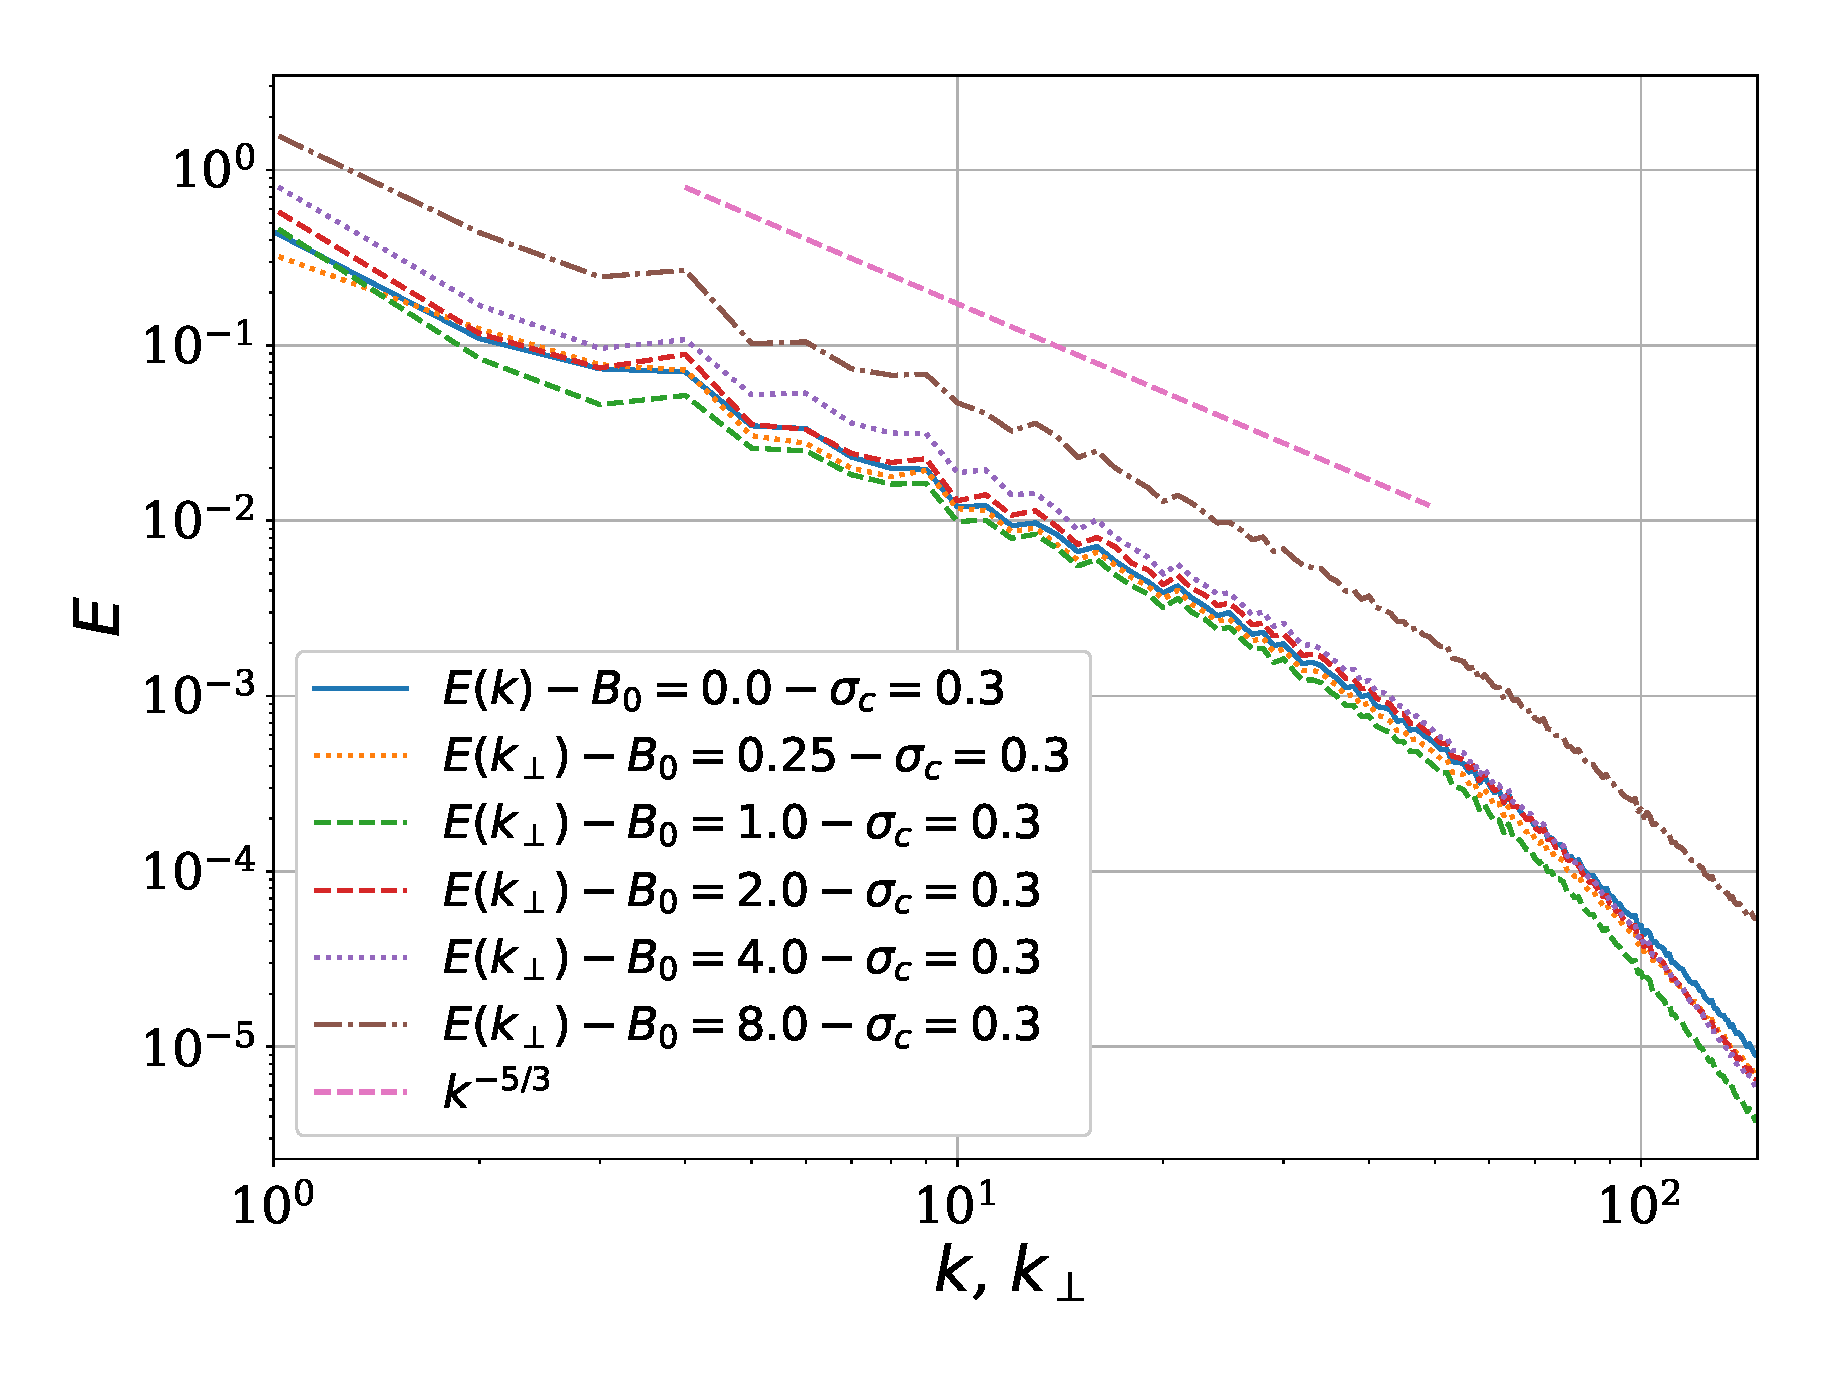
\includegraphics[width=\columnwidth]{P2/fig1_E.eps}
      \end{center}
    \end{minipage}
    \column{0.3\textwidth}
    \begin{minipage}[t]{1\textwidth}
      \begin{center}
        {\large $B_0 = 0$}\\
        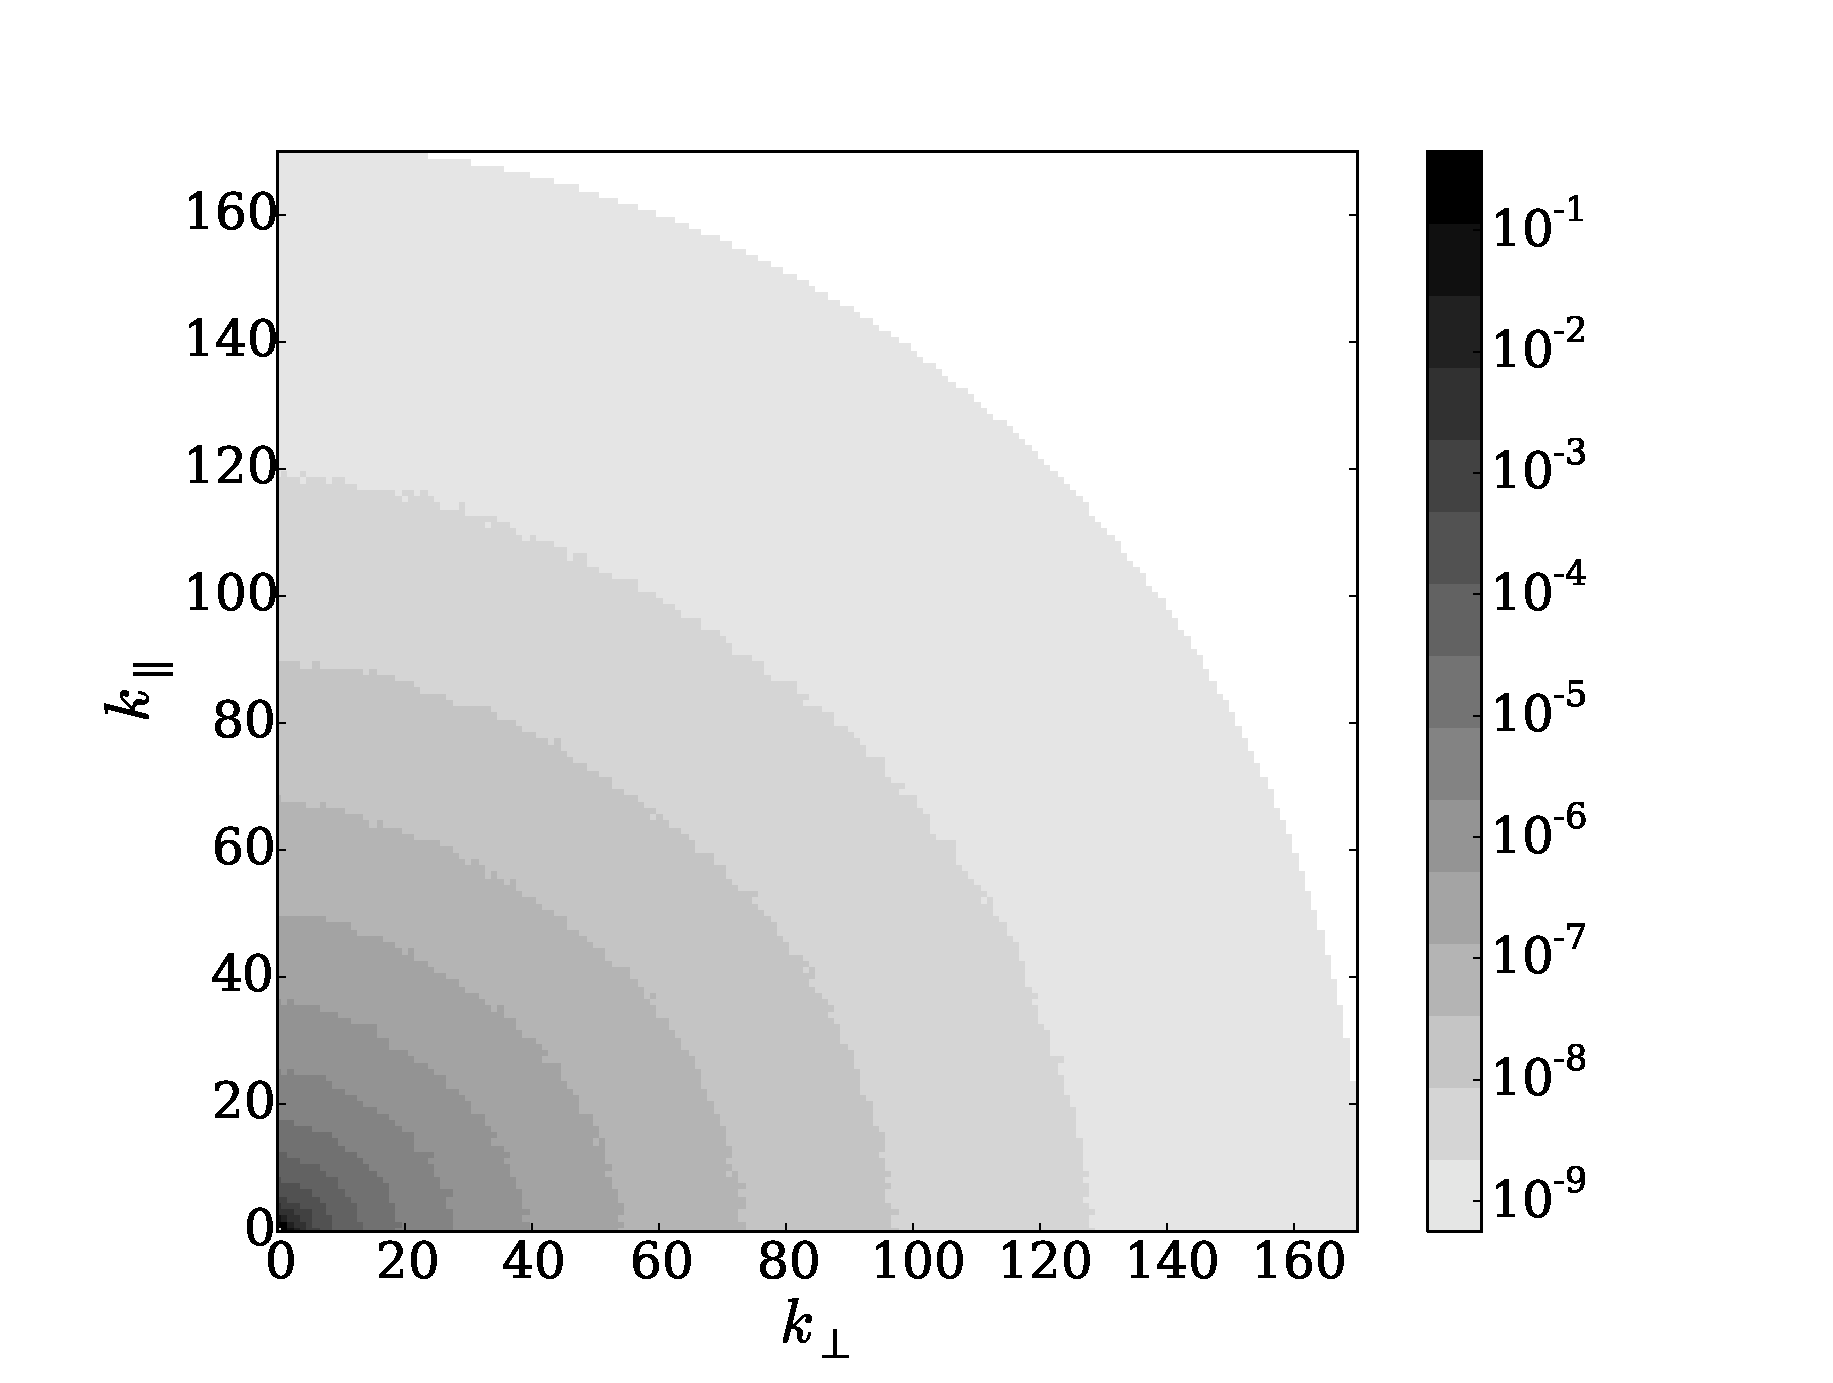
\includegraphics[width=\columnwidth]{P1/fig2_B0.eps} \\
        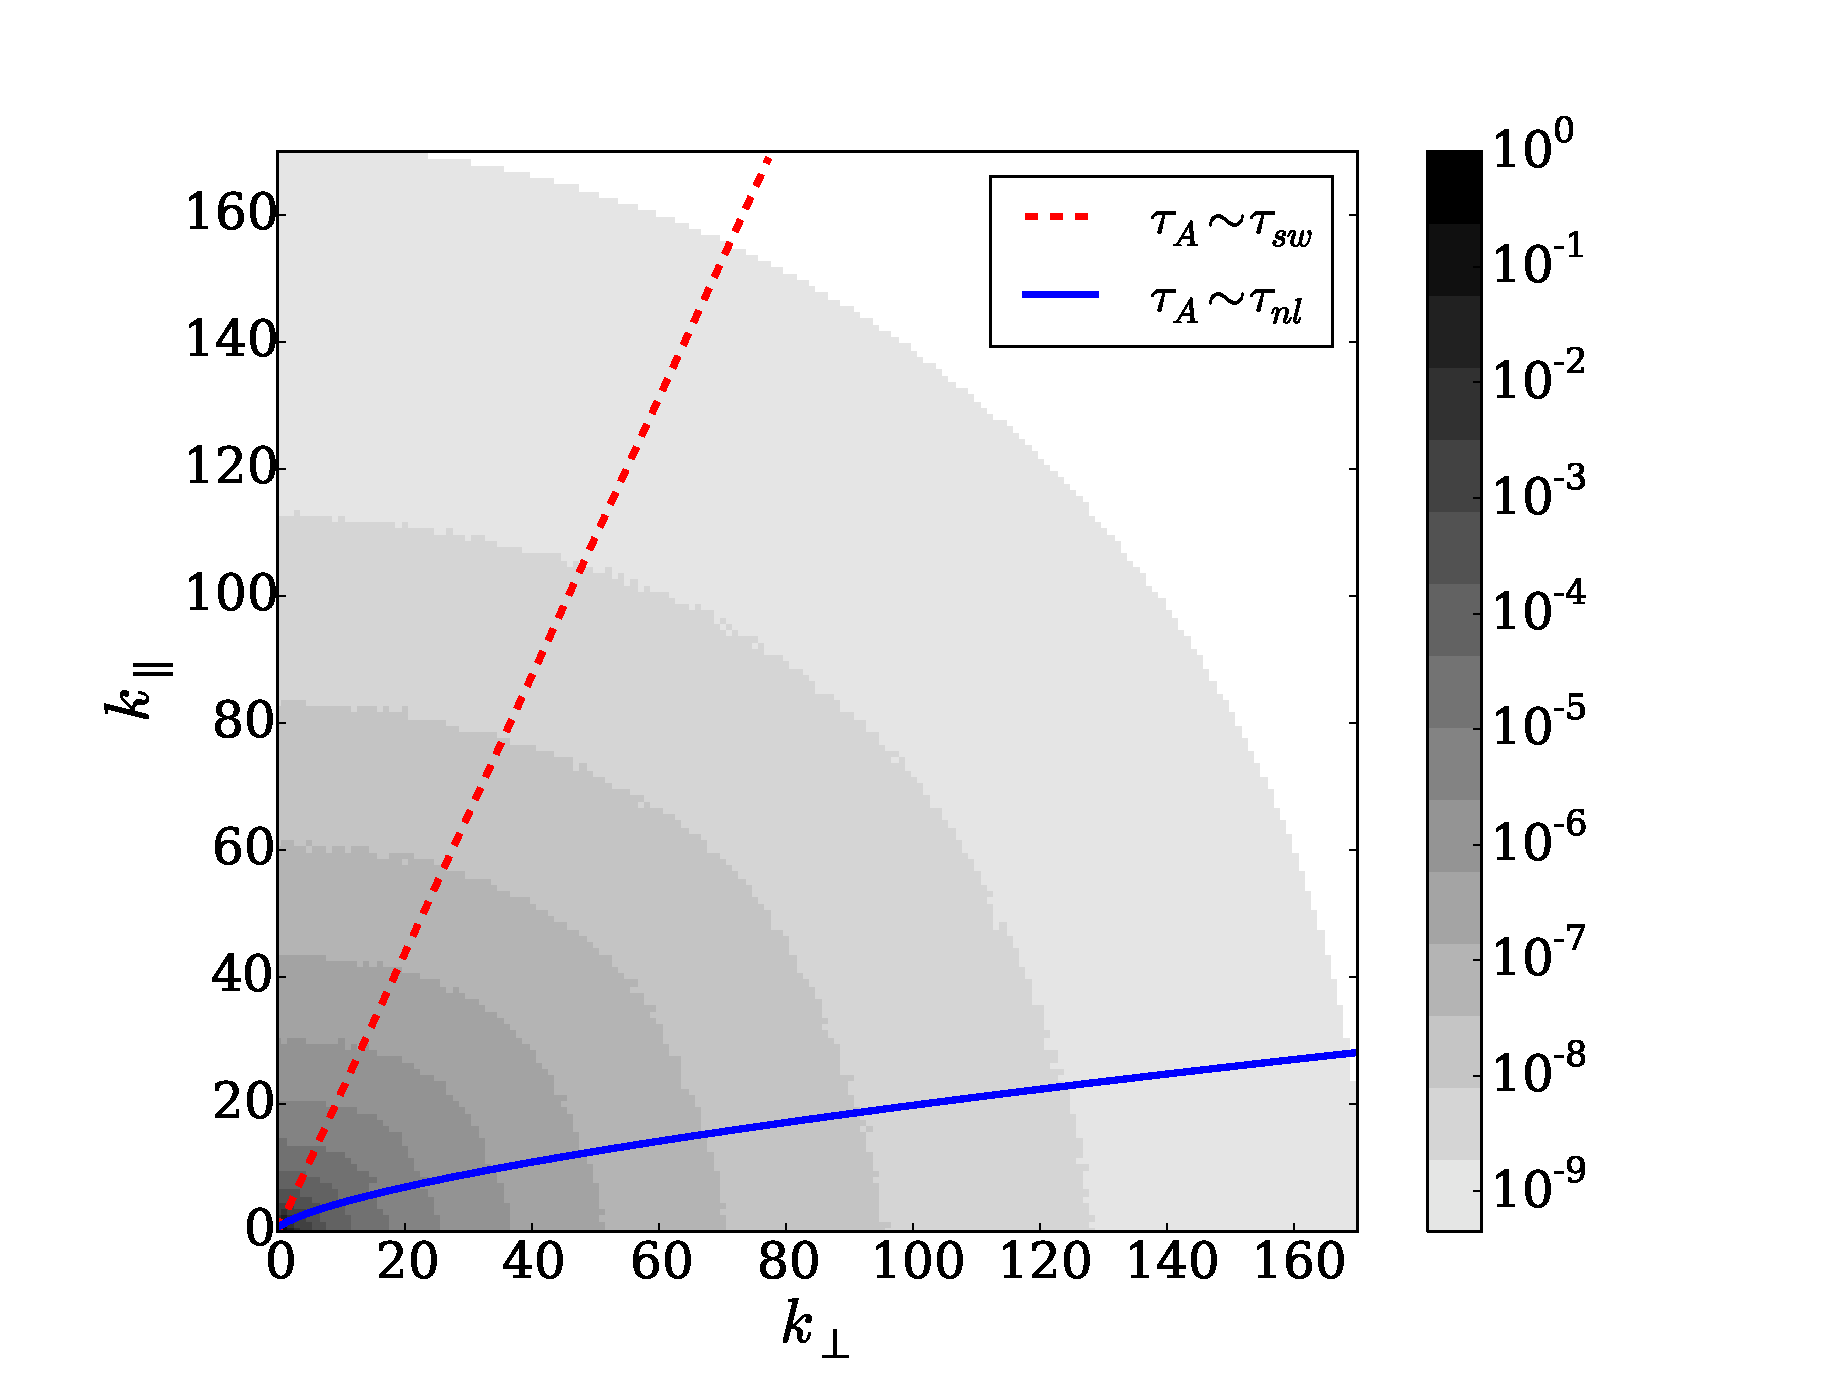
\includegraphics[width=\columnwidth]{P1/fig2_B1.eps} \\
        {\large $B_0 = 1$}
      \end{center}
    \end{minipage}
    \column{0.3\textwidth}
    \begin{minipage}[t]{1\textwidth}
      \begin{center}
        {\large $B_0 = 4$}\\
        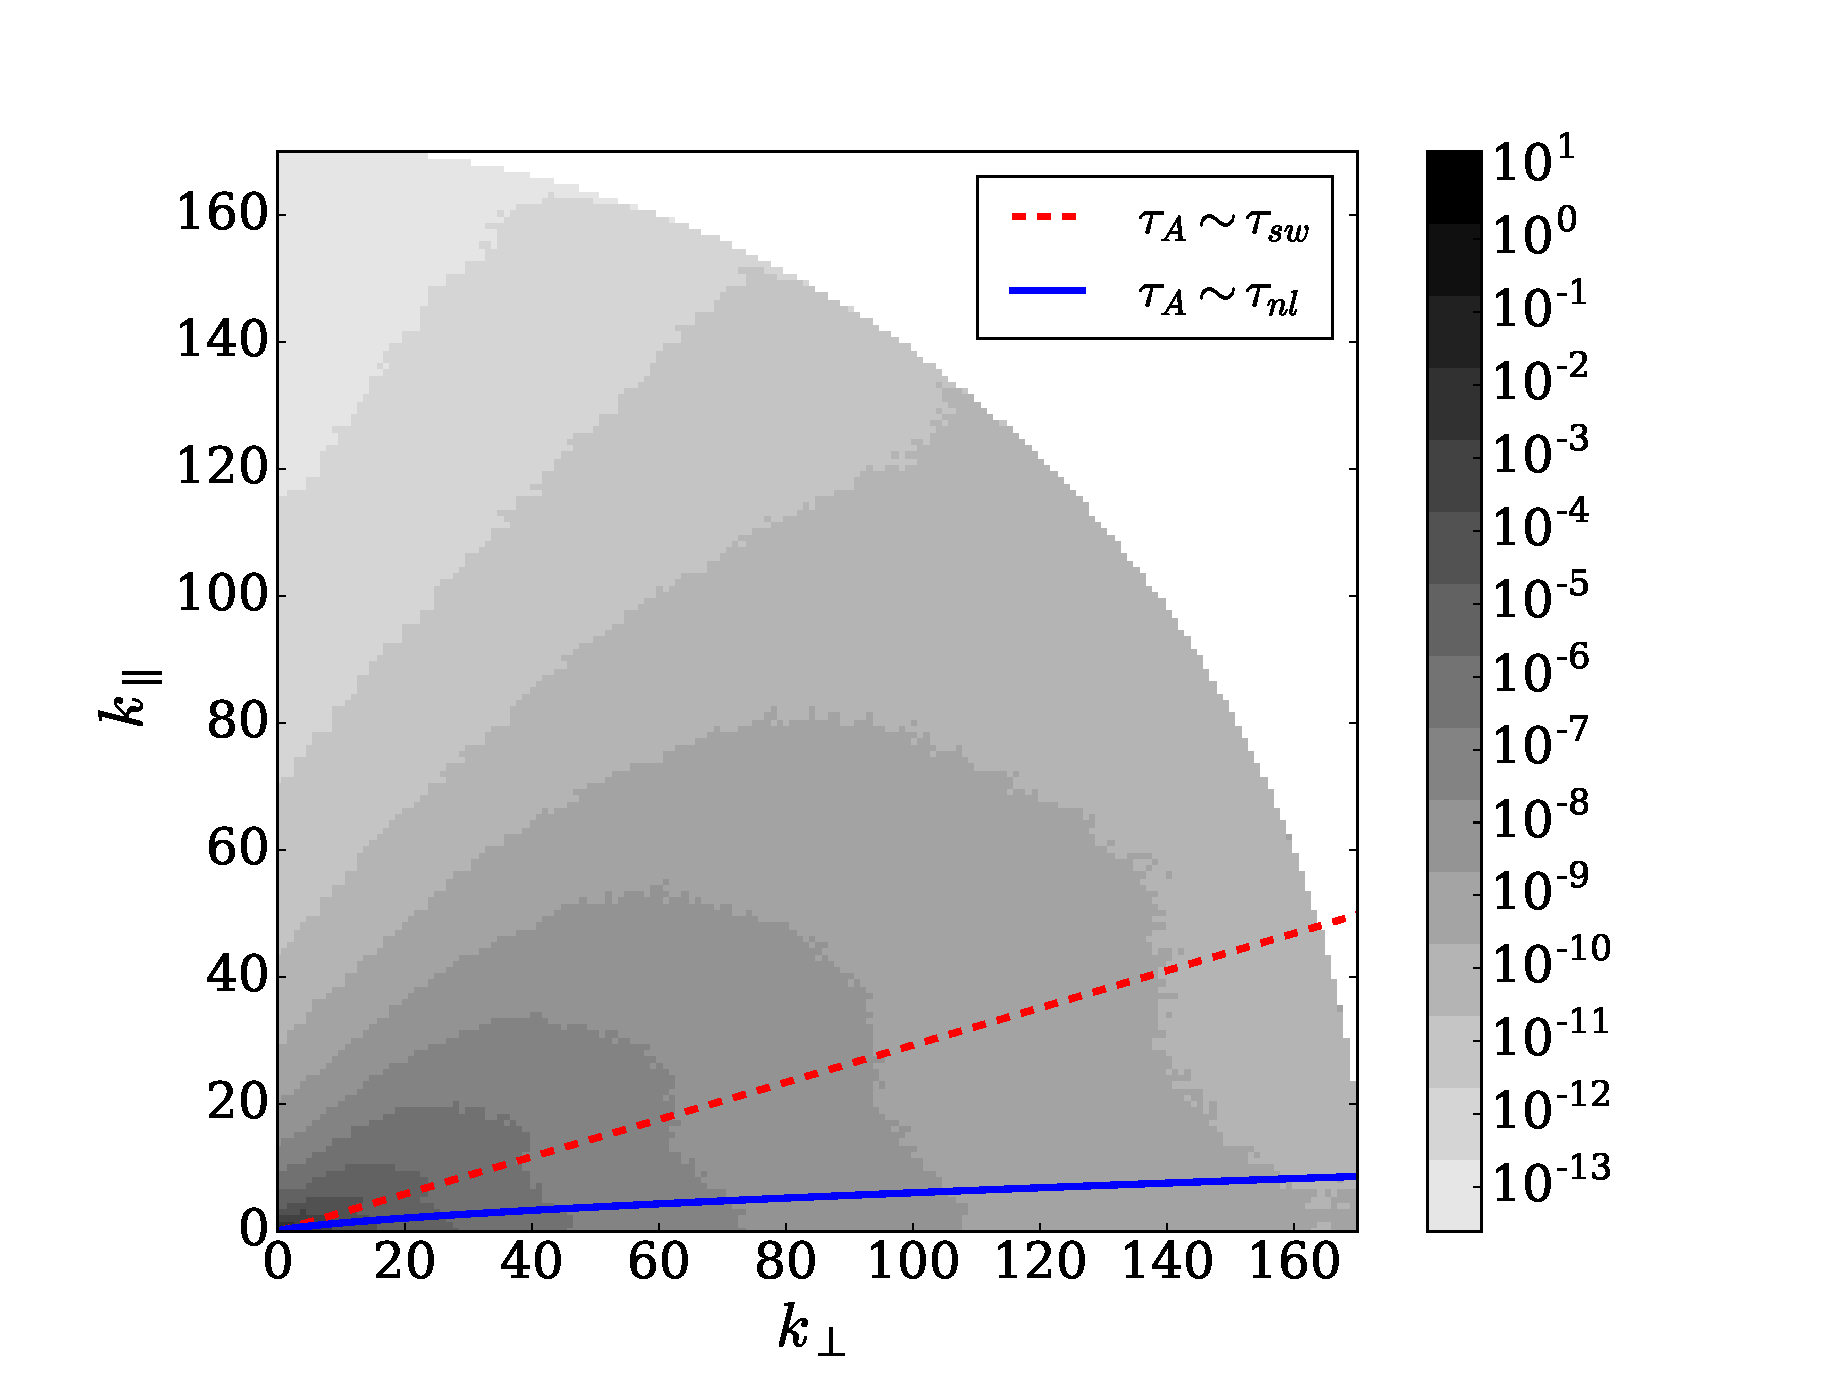
\includegraphics[width=\columnwidth]{P1/fig2_B4.eps} \\
        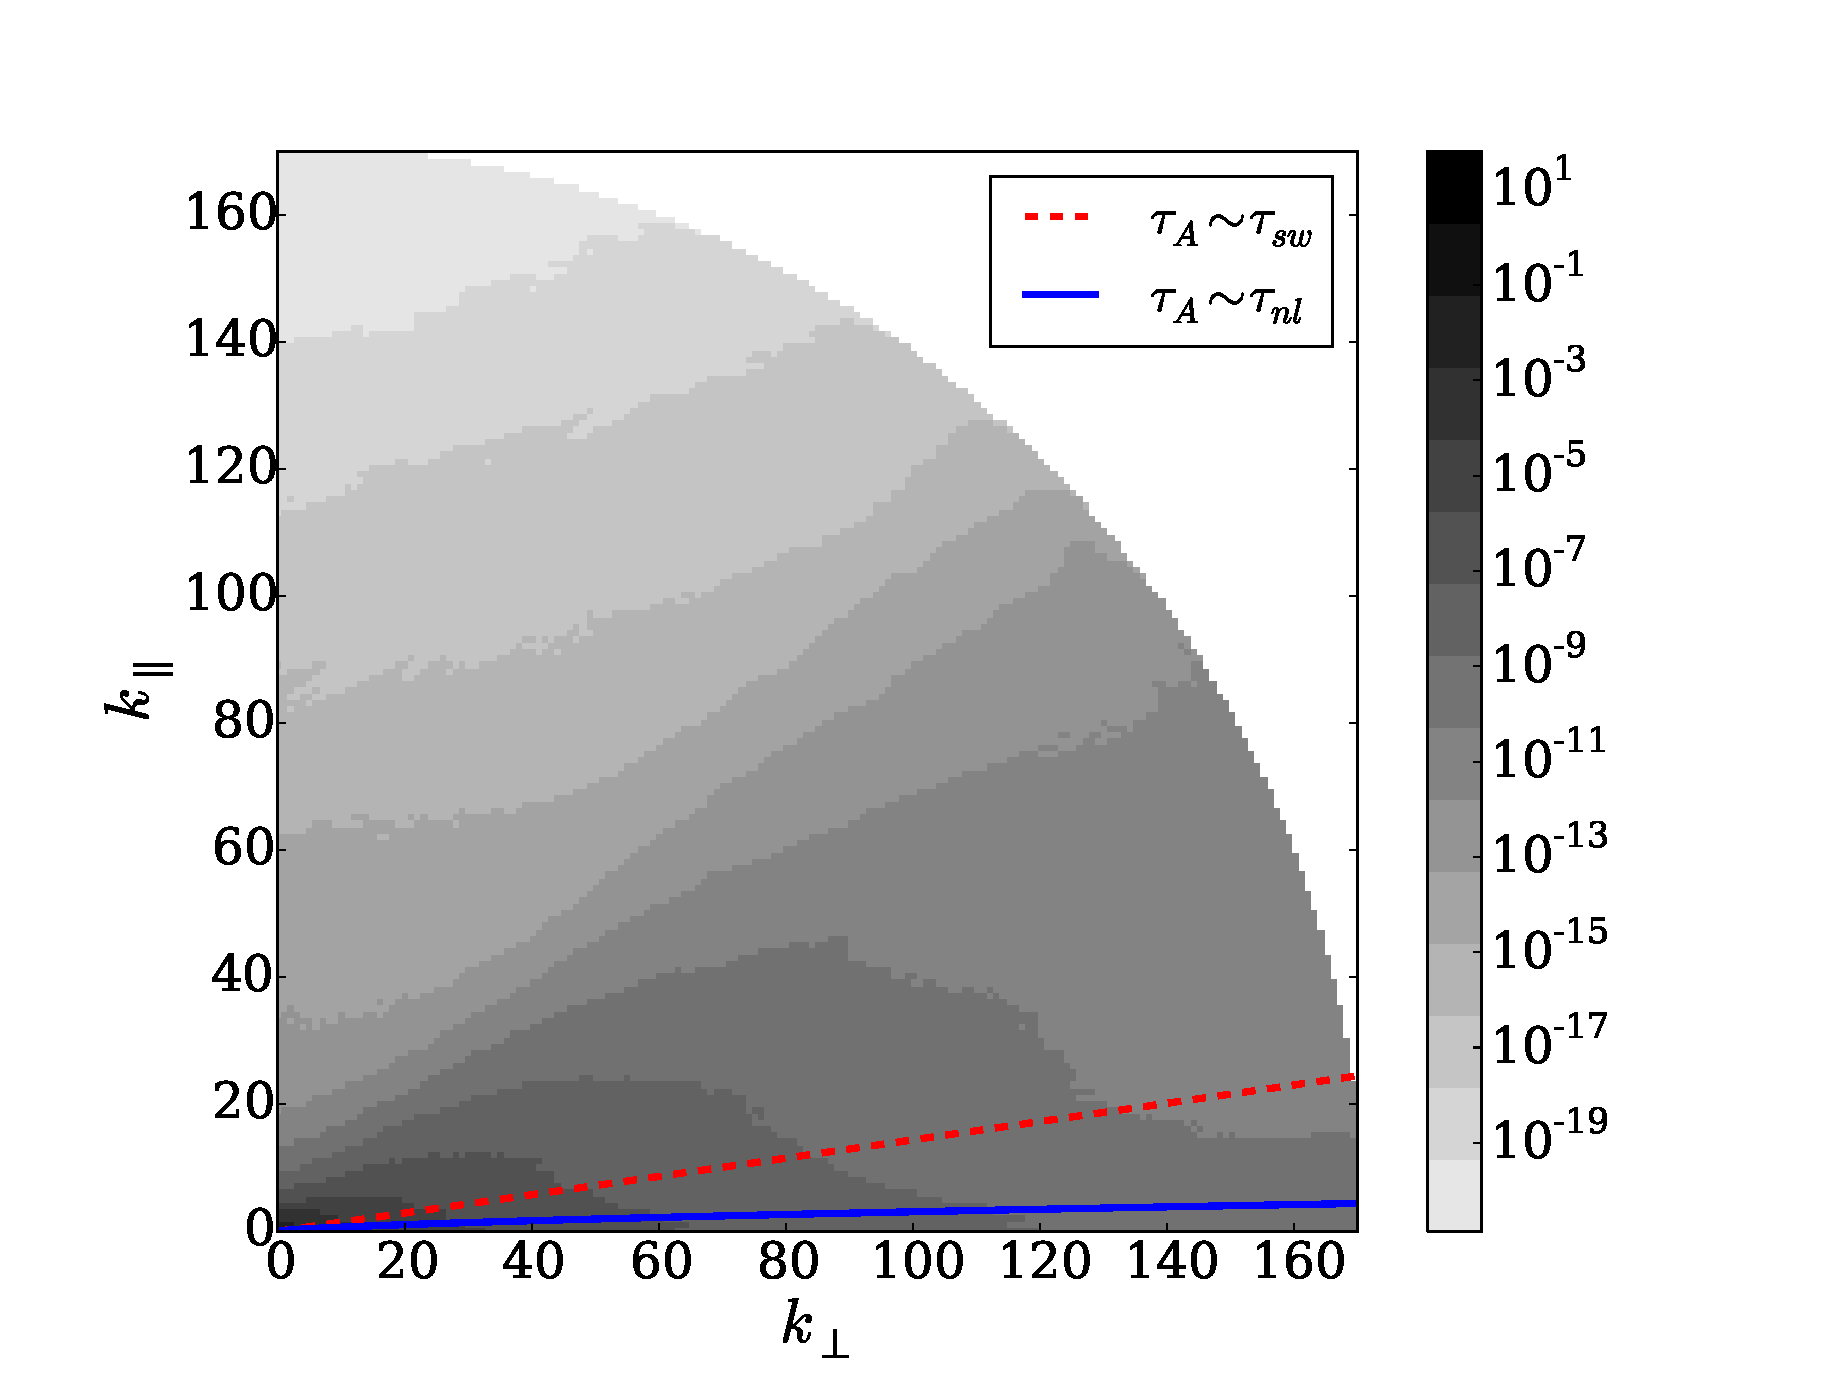
\includegraphics[width=\columnwidth]{P1/fig2_B8.eps} \\
        {\large $B_0 = 8$}
      \end{center}
    \end{minipage}
  \end{columns}
}
\note[itemize]{
  \item Los isocontornos cambian de
    forma a medida que cruzan cada una de estas líneas para $B_0$ grande.
  \item Aumento de anisotropía a medida que $B_0$ se incrementa, así
    como también la mayor superficie cubierta por modos en los que el
    período de Alfv\'en es el tiempo más rápido.  }




\frame{\frametitle{Espectros espacio-temporales}
}
\note[itemize]{
\item Acá están los principales resultados.
\item Espectro normalizado, con $k_\perp=0$ y en función de
  $k_\parallel$ y $\omega$.
}






\frame{\frametitle{Espectros espacio-temporales}
  {\large \underline{Espectro energético normalizado $E({\bf k}, \omega)/E({\bf k})$}}
  {\large, $B_0 = 0$}\vspace{10pt}
  \begin{columns}
    \column{0.5\textwidth}
    \begin{minipage}[t]{1\textwidth}
      \begin{center}
        {$\vec{z}^-$, $\sigma_c = 0.3$} \\
        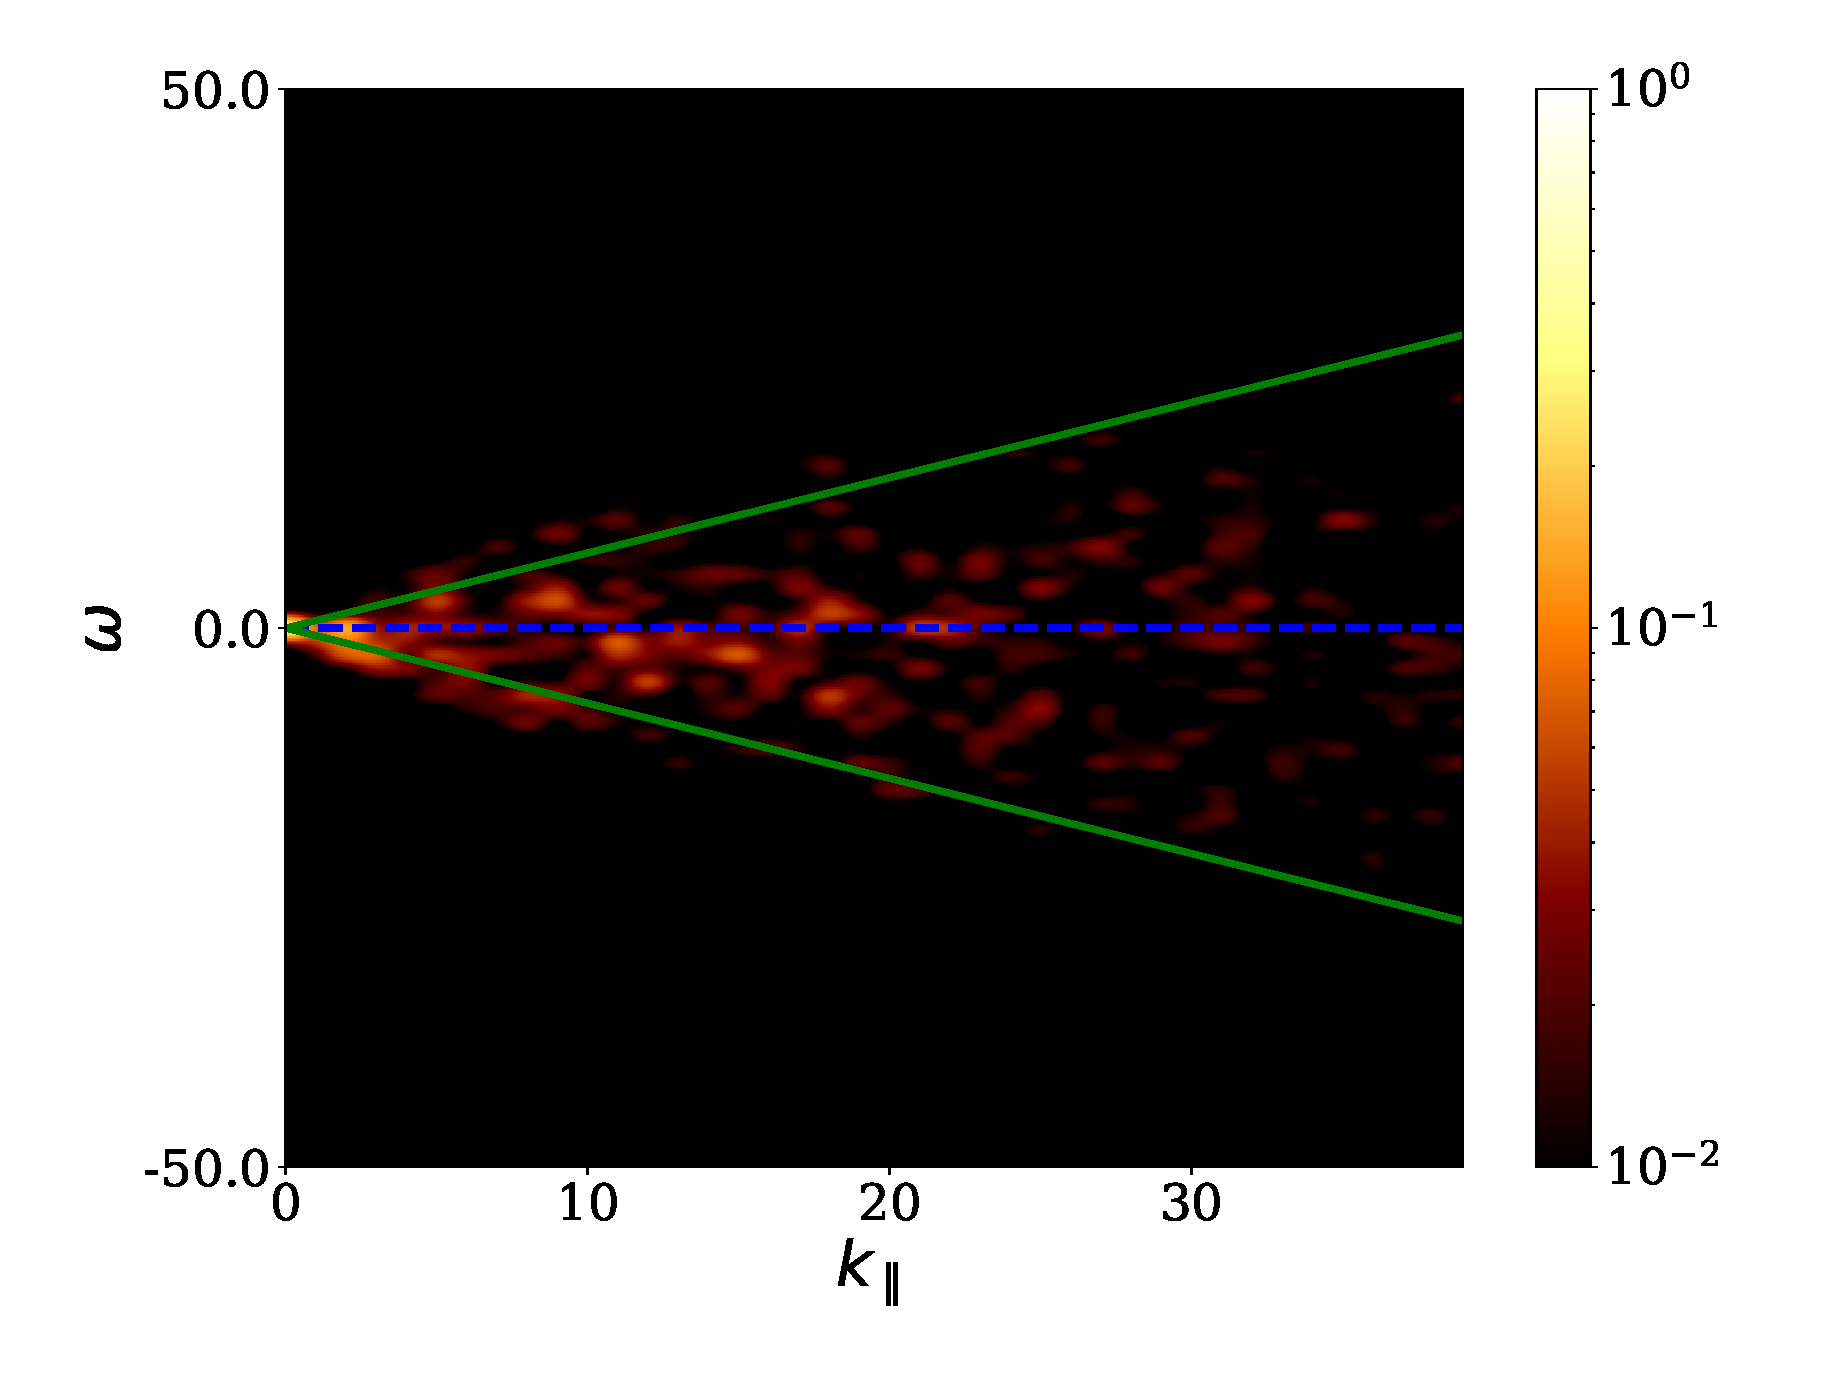
\includegraphics[width=0.65\textwidth]{{P2/fig3_B0.0_y_Hc0.3_zm_kperp0}.eps} \\
        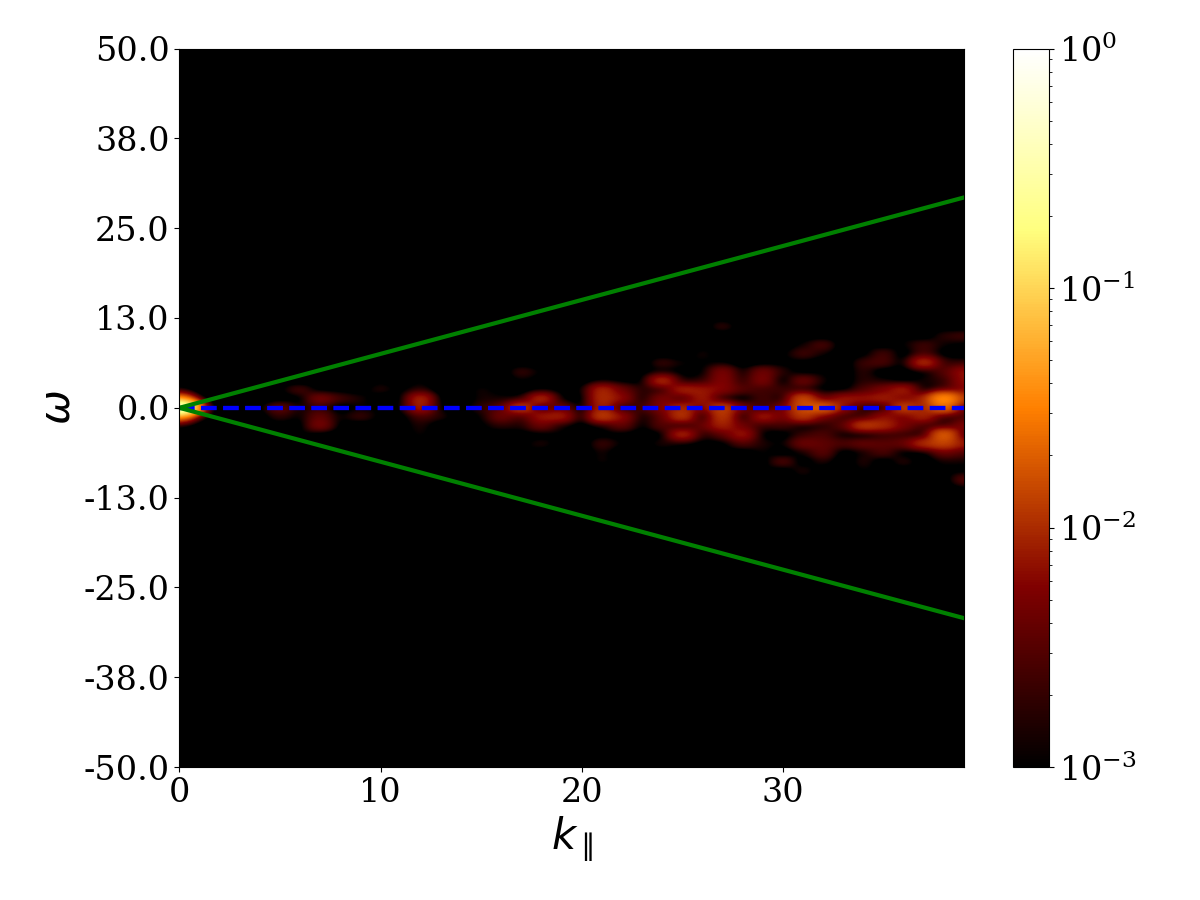
\includegraphics[width=0.65\textwidth]{{P2/fig3_B0.0_y_Hc0.9_zm_kperp0}.eps} \\
        {$\vec{z}^-$, $\sigma_c = 0.9$}
      \end{center}
    \end{minipage}
    \column{0.5\textwidth}
    \begin{minipage}[t]{1\textwidth}
      \begin{center}
        {$\vec{z}^+$, $\sigma_c = 0.3$} \\
        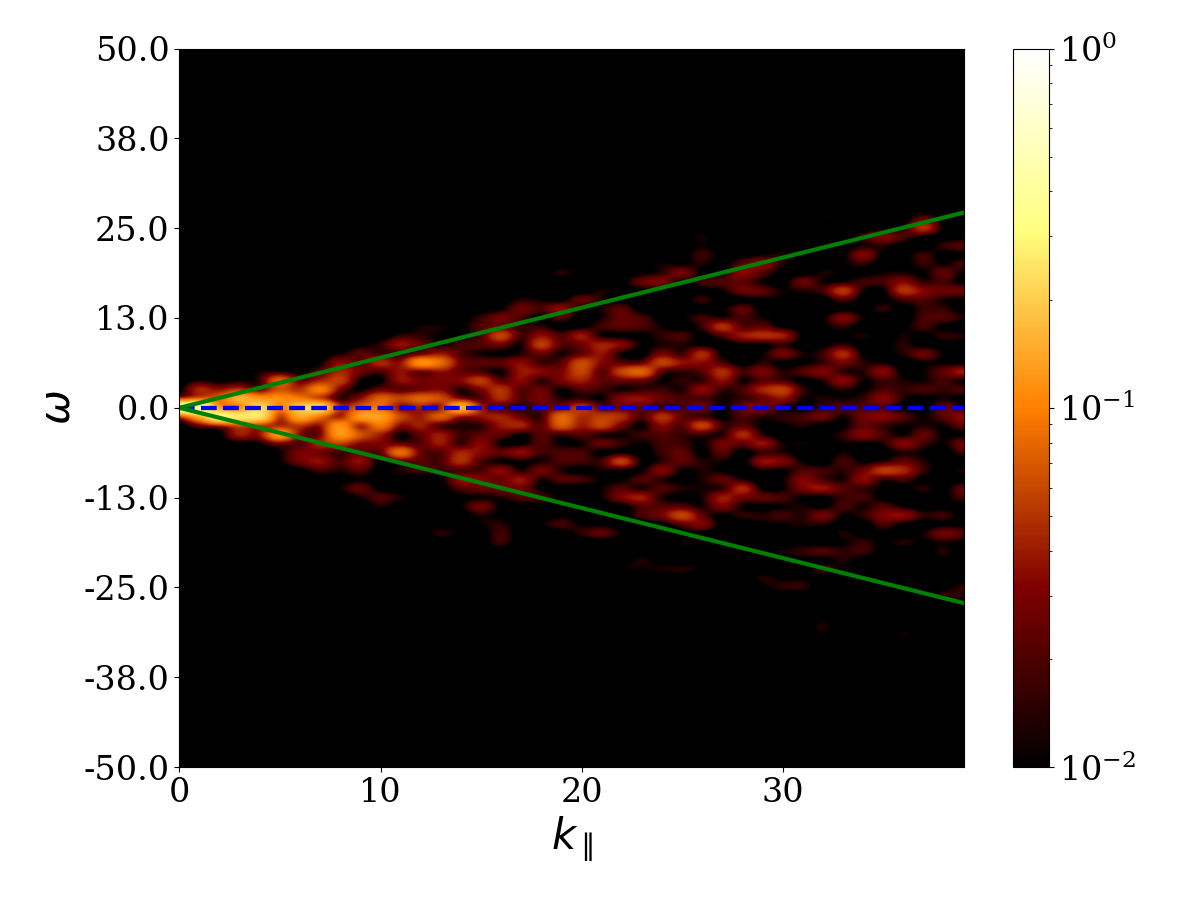
\includegraphics[width=0.65\textwidth]{{P2/fig3_B0.0_y_Hc0.3_zp_kperp0}.eps} \\
        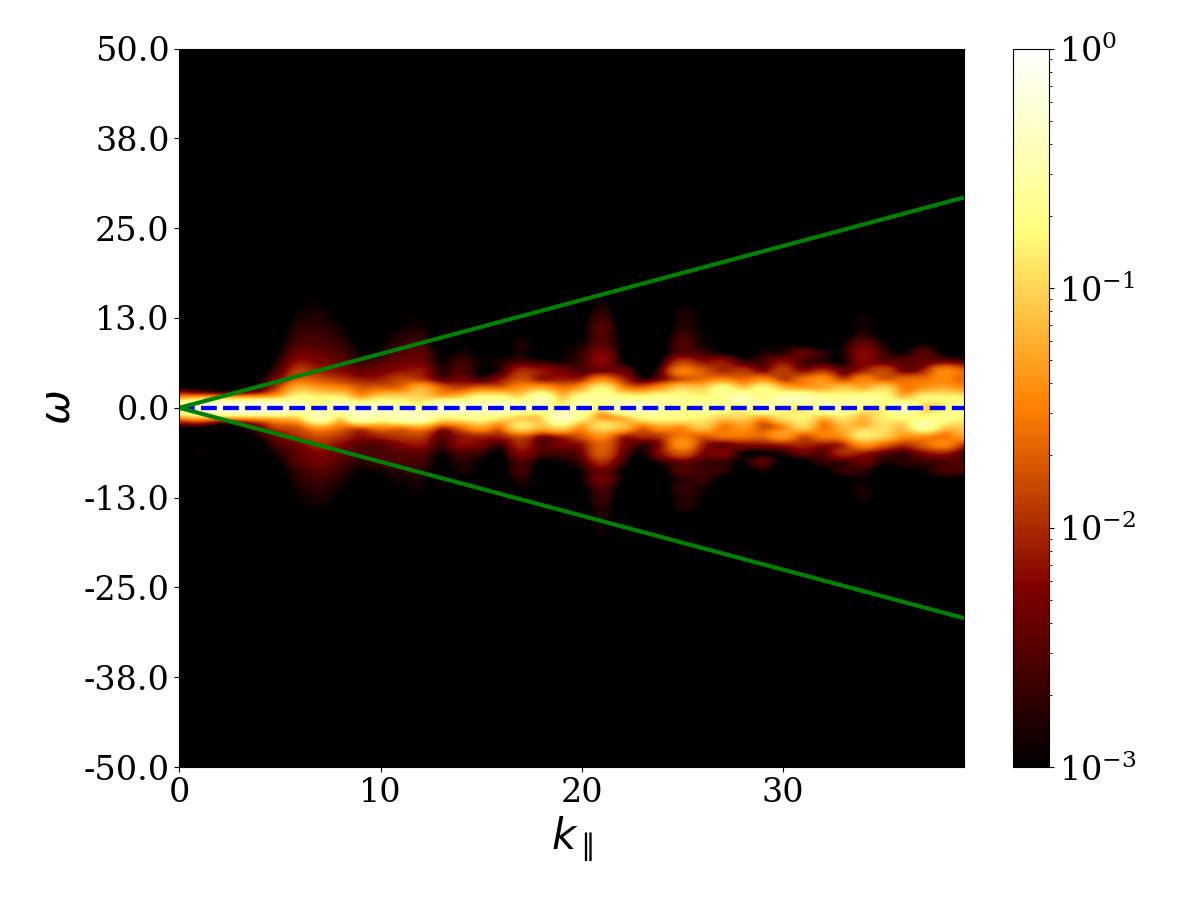
\includegraphics[width=0.65\textwidth]{{P2/fig3_B0.0_y_Hc0.9_zp_kperp0}.eps} \\
        {$\vec{z}^+$, $\sigma_c = 0.9$}
      \end{center}
    \end{minipage}
  \end{columns}
}
\note[itemize]{
\item $k_\perp=0$ fijo. Líneas de \emph{sweeping} y Alfvén.
\item Espectro: Fourier en $t$ y $r$ de $\vec{z}^\pm$. Acumulación de
  energía.
\item Alfvén ($\omega=0$) indistinguible de los modos lentos (ej, \textit{eddies}).
\item E en todo el embudo, evidenciando turbulencia fuerte
  en todas las escalas, más que turbulencia de ondas o propagación
  lineal de ondas.
\item Para $\sigma_c$ grande, energía en $\omega\approx 0$ y en
  $\vec{z}^+$.
\item Para $B_0=0$ y $\sigma_c=0$, la escala de tiempo dominante es la
  del \textit{sweeping}, mientras que para grandes valores de
  $\sigma_c$, se vuelven dominantes o bien la escala temporal no
  lineal o el tiempo de Alfvén.
\item Mayor $\sigma_c$, más E en $\vec{z}^+$.
}



\frame{\frametitle{Espectros espacio-temporales}
  {\large \underline{Espectro energético normalizado $E({\bf k}, \omega)/E({\bf k})$}}
  {\large, $B_0 = 1$}\vspace{10pt}
  \begin{columns}
    \column{0.33\textwidth}
    \begin{minipage}[t]{1\textwidth}
      \begin{center}
        {$\vec{z}^+$, $\sigma_c = 0.0$} \\
        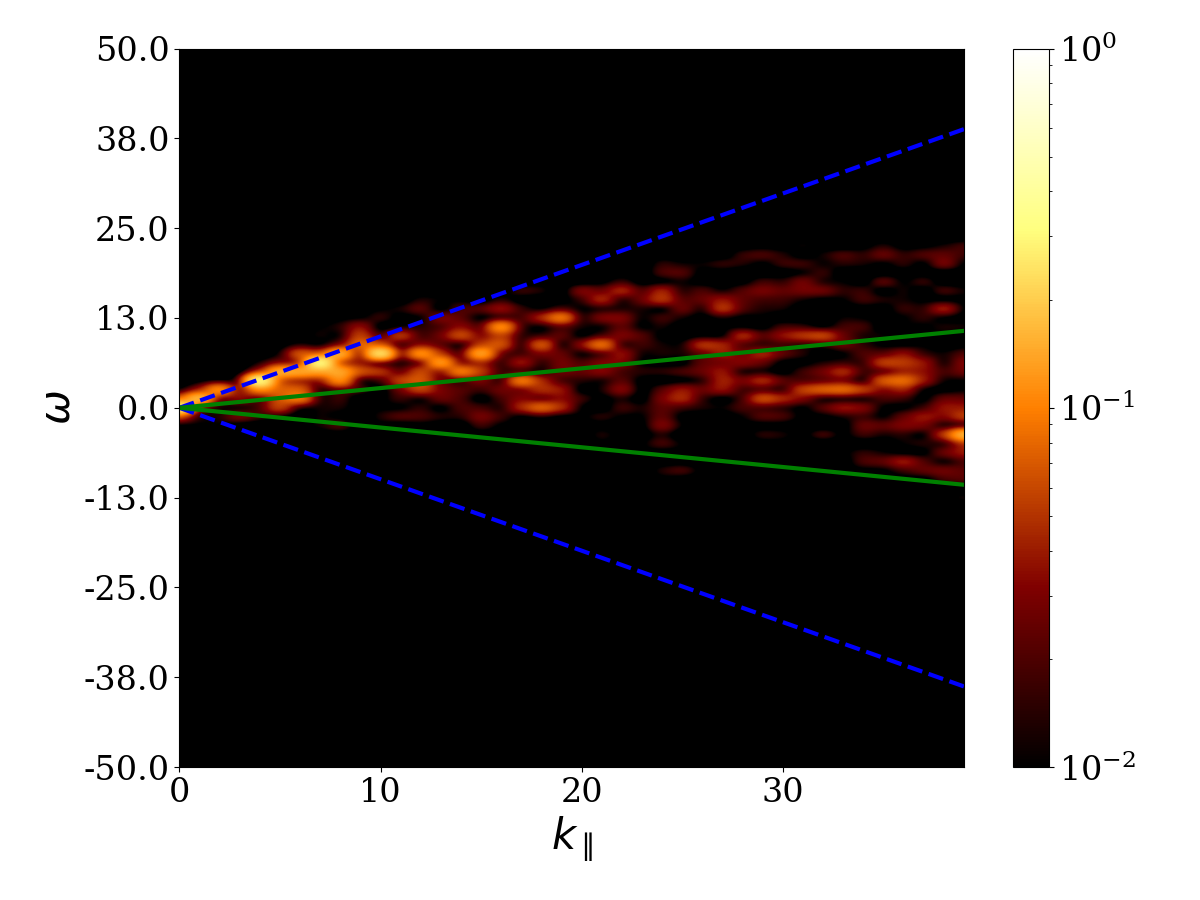
\includegraphics[width=0.95\textwidth]{{P2/fig3_B1.0_y_Hc0.0_zp_kperp0}.eps} \\
        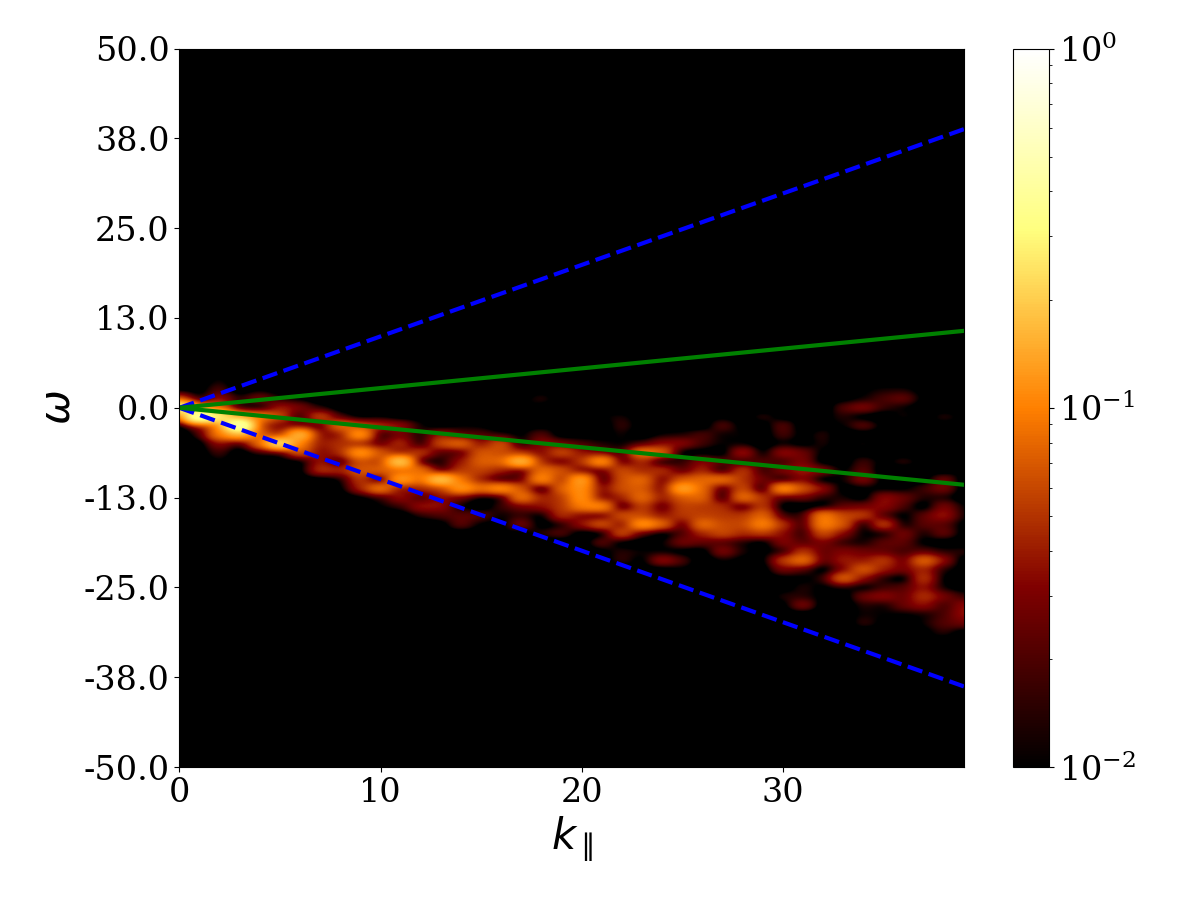
\includegraphics[width=0.95\textwidth]{{P2/fig3_B1.0_y_Hc0.0_zm_kperp0}.eps} \\
        {$\vec{z}^-$, $\sigma_c = 0.0$}
      \end{center}
    \end{minipage}
    \column{0.33\textwidth}
    \begin{minipage}[t]{1\textwidth}
      \begin{center}
        {$\vec{z}^+$, $\sigma_c = 0.3$} \\
        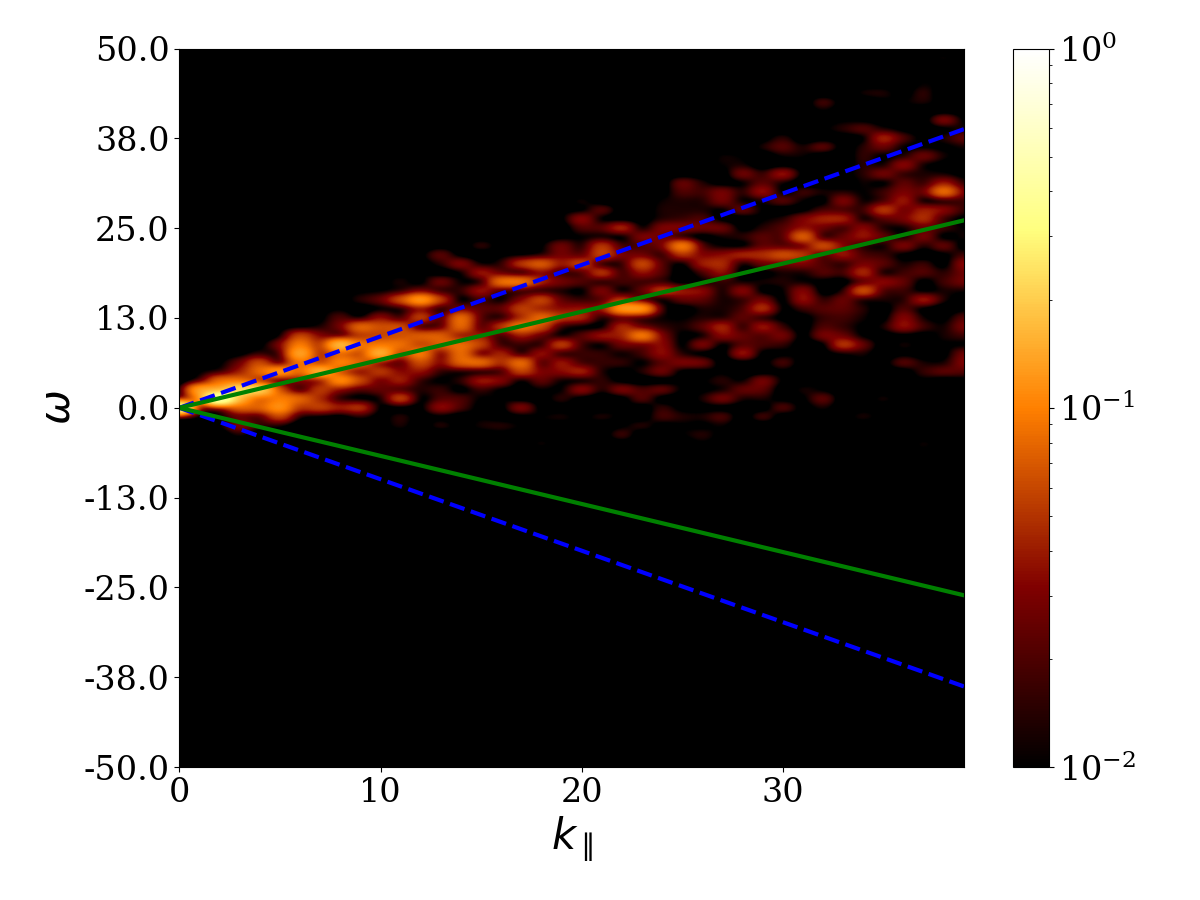
\includegraphics[width=0.95\textwidth]{{P2/fig3_B1.0_y_Hc0.3_zp_kperp0}.eps} \\
        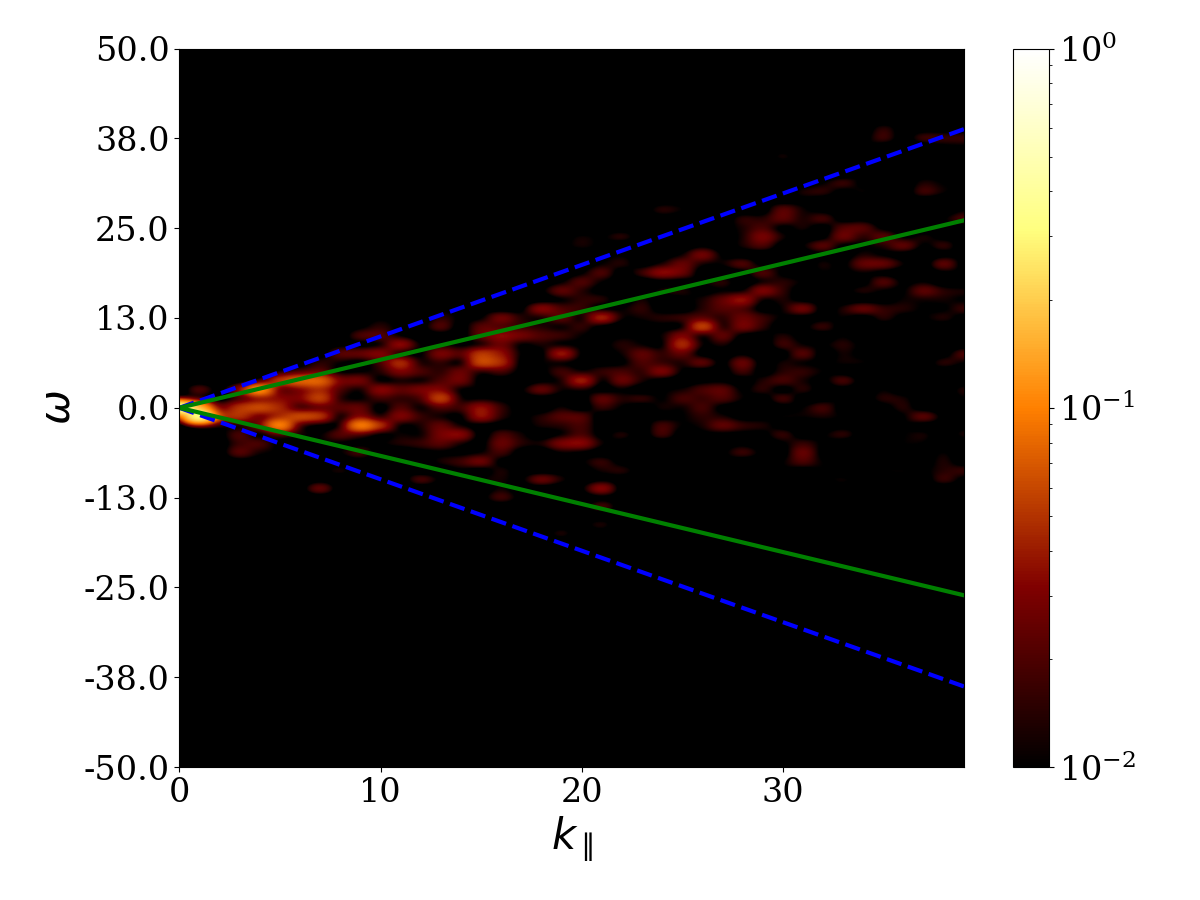
\includegraphics[width=0.95\textwidth]{{P2/fig3_B1.0_y_Hc0.3_zm_kperp0}.eps} \\
        {$\vec{z}^-$, $\sigma_c = 0.3$}
      \end{center}
    \end{minipage}
    \column{0.33\textwidth}
    \begin{minipage}[t]{1\textwidth}
      \begin{center}
        {$\vec{z}^+$, $\sigma_c = 0.9$} \\
        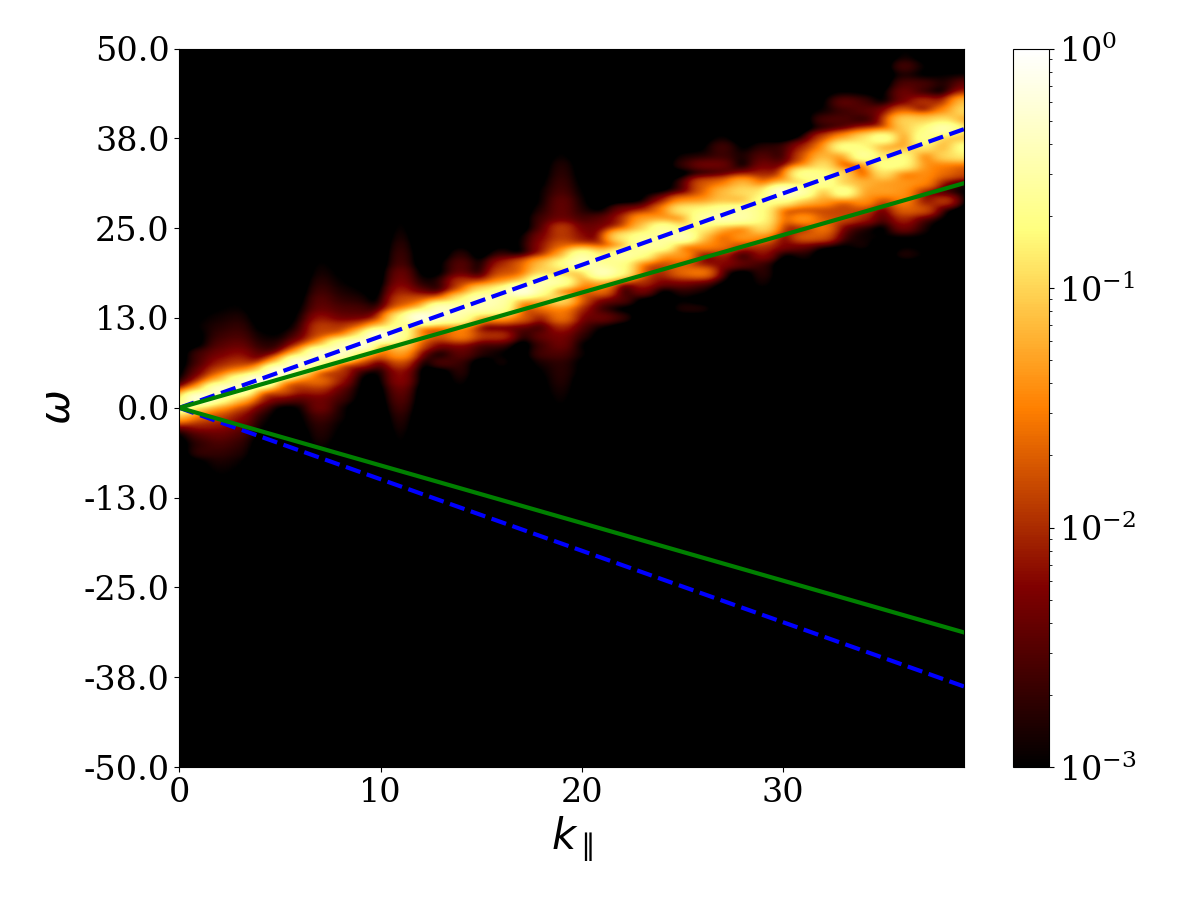
\includegraphics[width=0.95\textwidth]{{P2/fig3_B1.0_y_Hc0.9_zp_kperp0}.eps} \\
        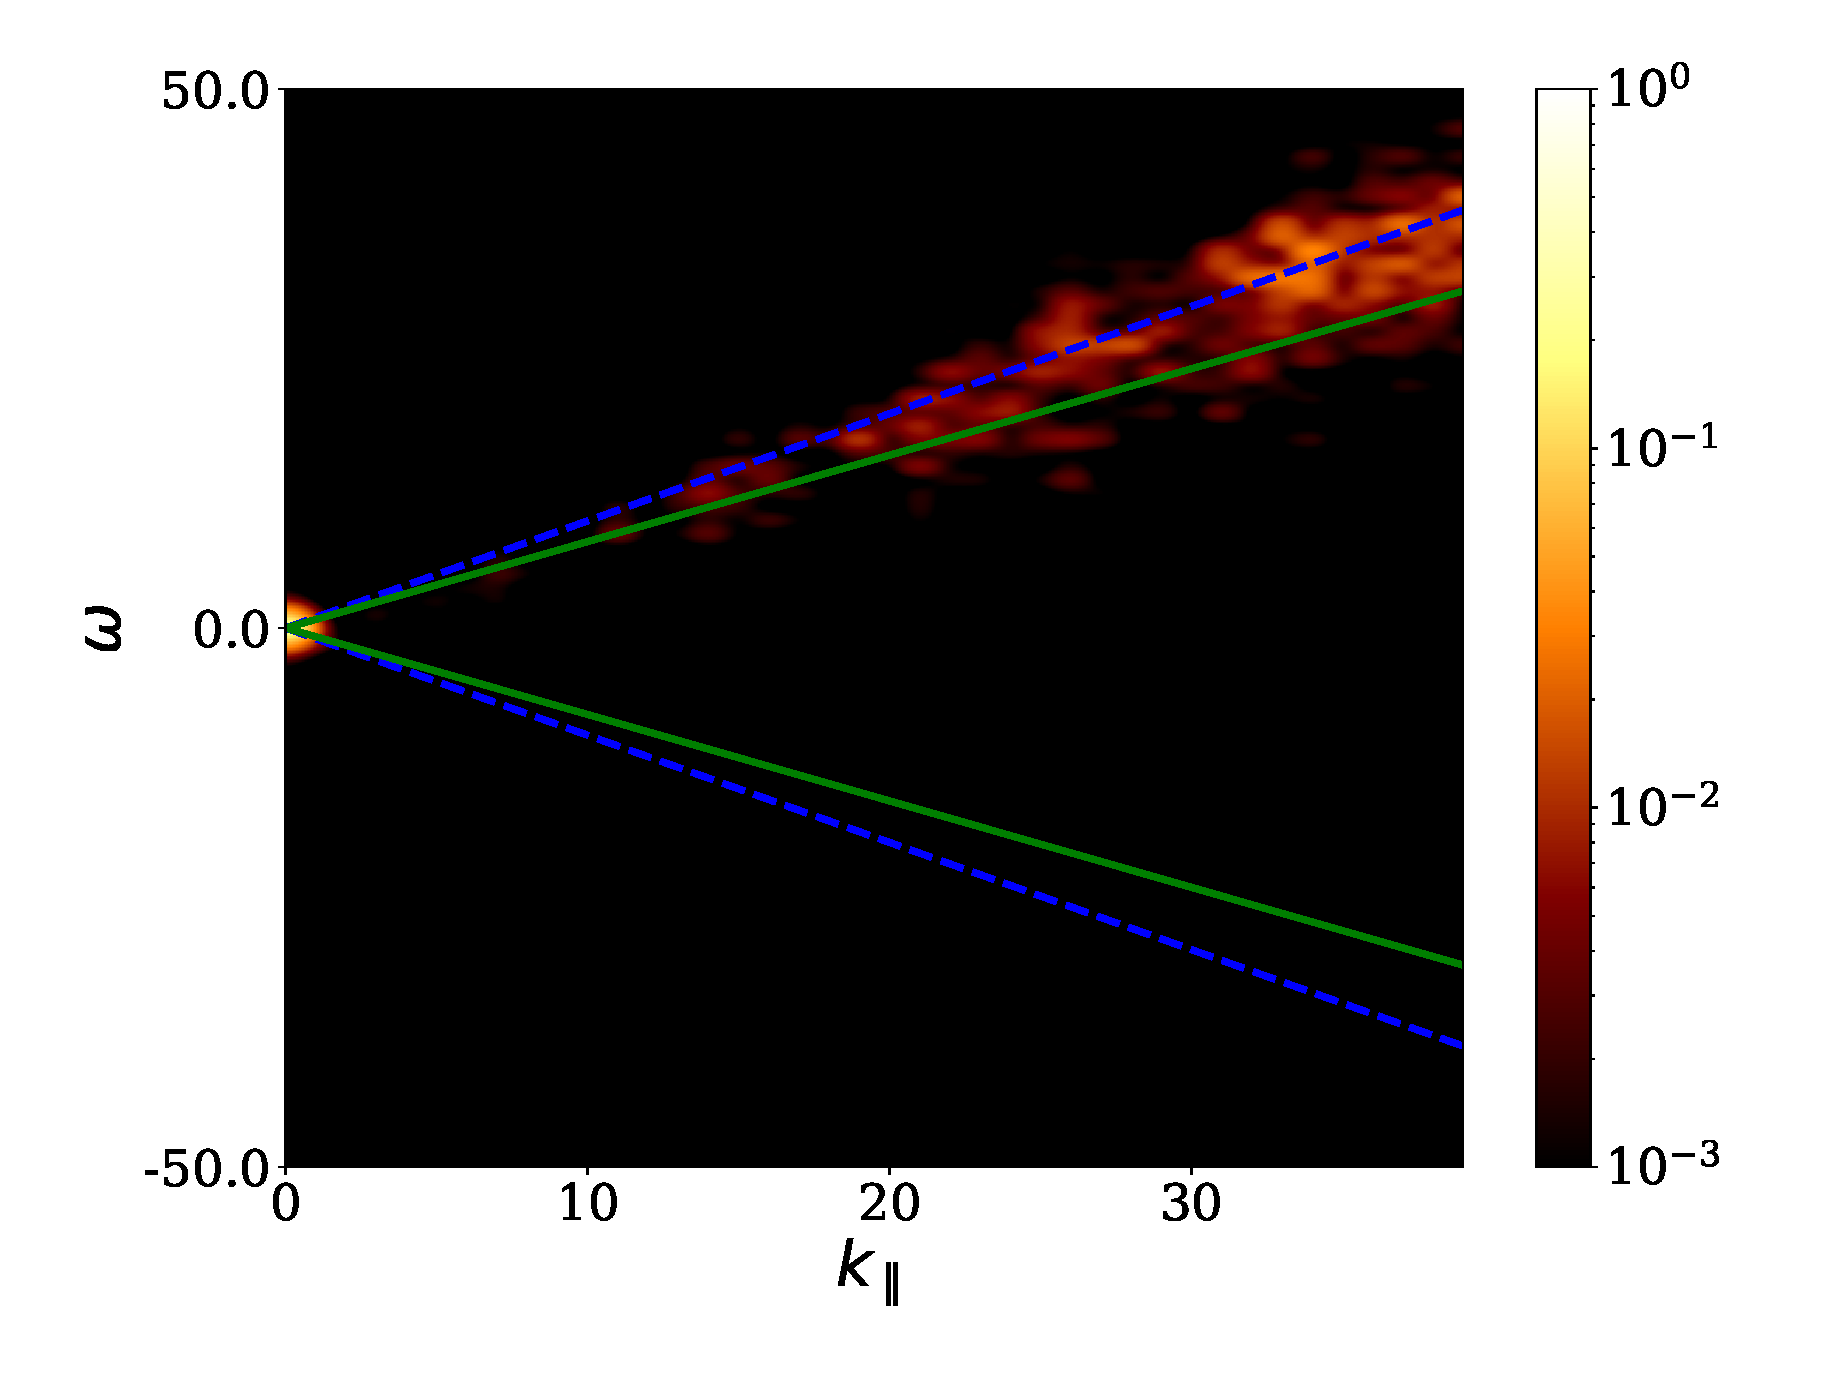
\includegraphics[width=0.95\textwidth]{{P2/fig3_B1.0_y_Hc0.9_zm_kperp0}.eps} \\
        {$\vec{z}^-$, $\sigma_c = 0.9$}
      \end{center}
    \end{minipage}
  \end{columns}
}
\note[itemize]{
\item $\sigma_c = 0$, poco Alfvén. Propagación en direcciones
  correctas: $\vec{z}^+$ antiparalelamente, $\vec{z}^-$,
  paralelamente. 
\item $\sigma_c =0.3$ y $0.9$, E en Alfvén.
\item Contrapropagación de ondas: tanto el campo $\vec{z}^+$
  como el $\vec{z}^-$ se propagan en la misma dirección, antiparalela
  al campo guía.
\item Para el caso con $\sigma_c = 0.9$, ambos campos $\vec{z}^+$ y
  $\vec{z}^-$ siguen la misma relación de dispersión $\omega \approx +
  \vec{V}_A\cdot\vec{k}$, y las excitaciones de Alfv\'en dominan sobre
  todas las escalas.
\item Más $B_0$, relevancia del \textit{sweeping} aleatorio decrece, y
  las ondas de Alfvén se vuelven más importantes.
}



\frame{\frametitle{Espectros espacio-temporales}
  {\large \underline{Espectro energético normalizado $E({\bf k}, \omega)/E({\bf k})$}}
  {\large, $B_0 = 0.25$}\vspace{10pt}
  \begin{columns}
    \column{0.33\textwidth}
    \begin{minipage}[t]{1\textwidth}
      \begin{center}
        {$\vec{z}^+$, $\sigma_c = 0.0$} \\
        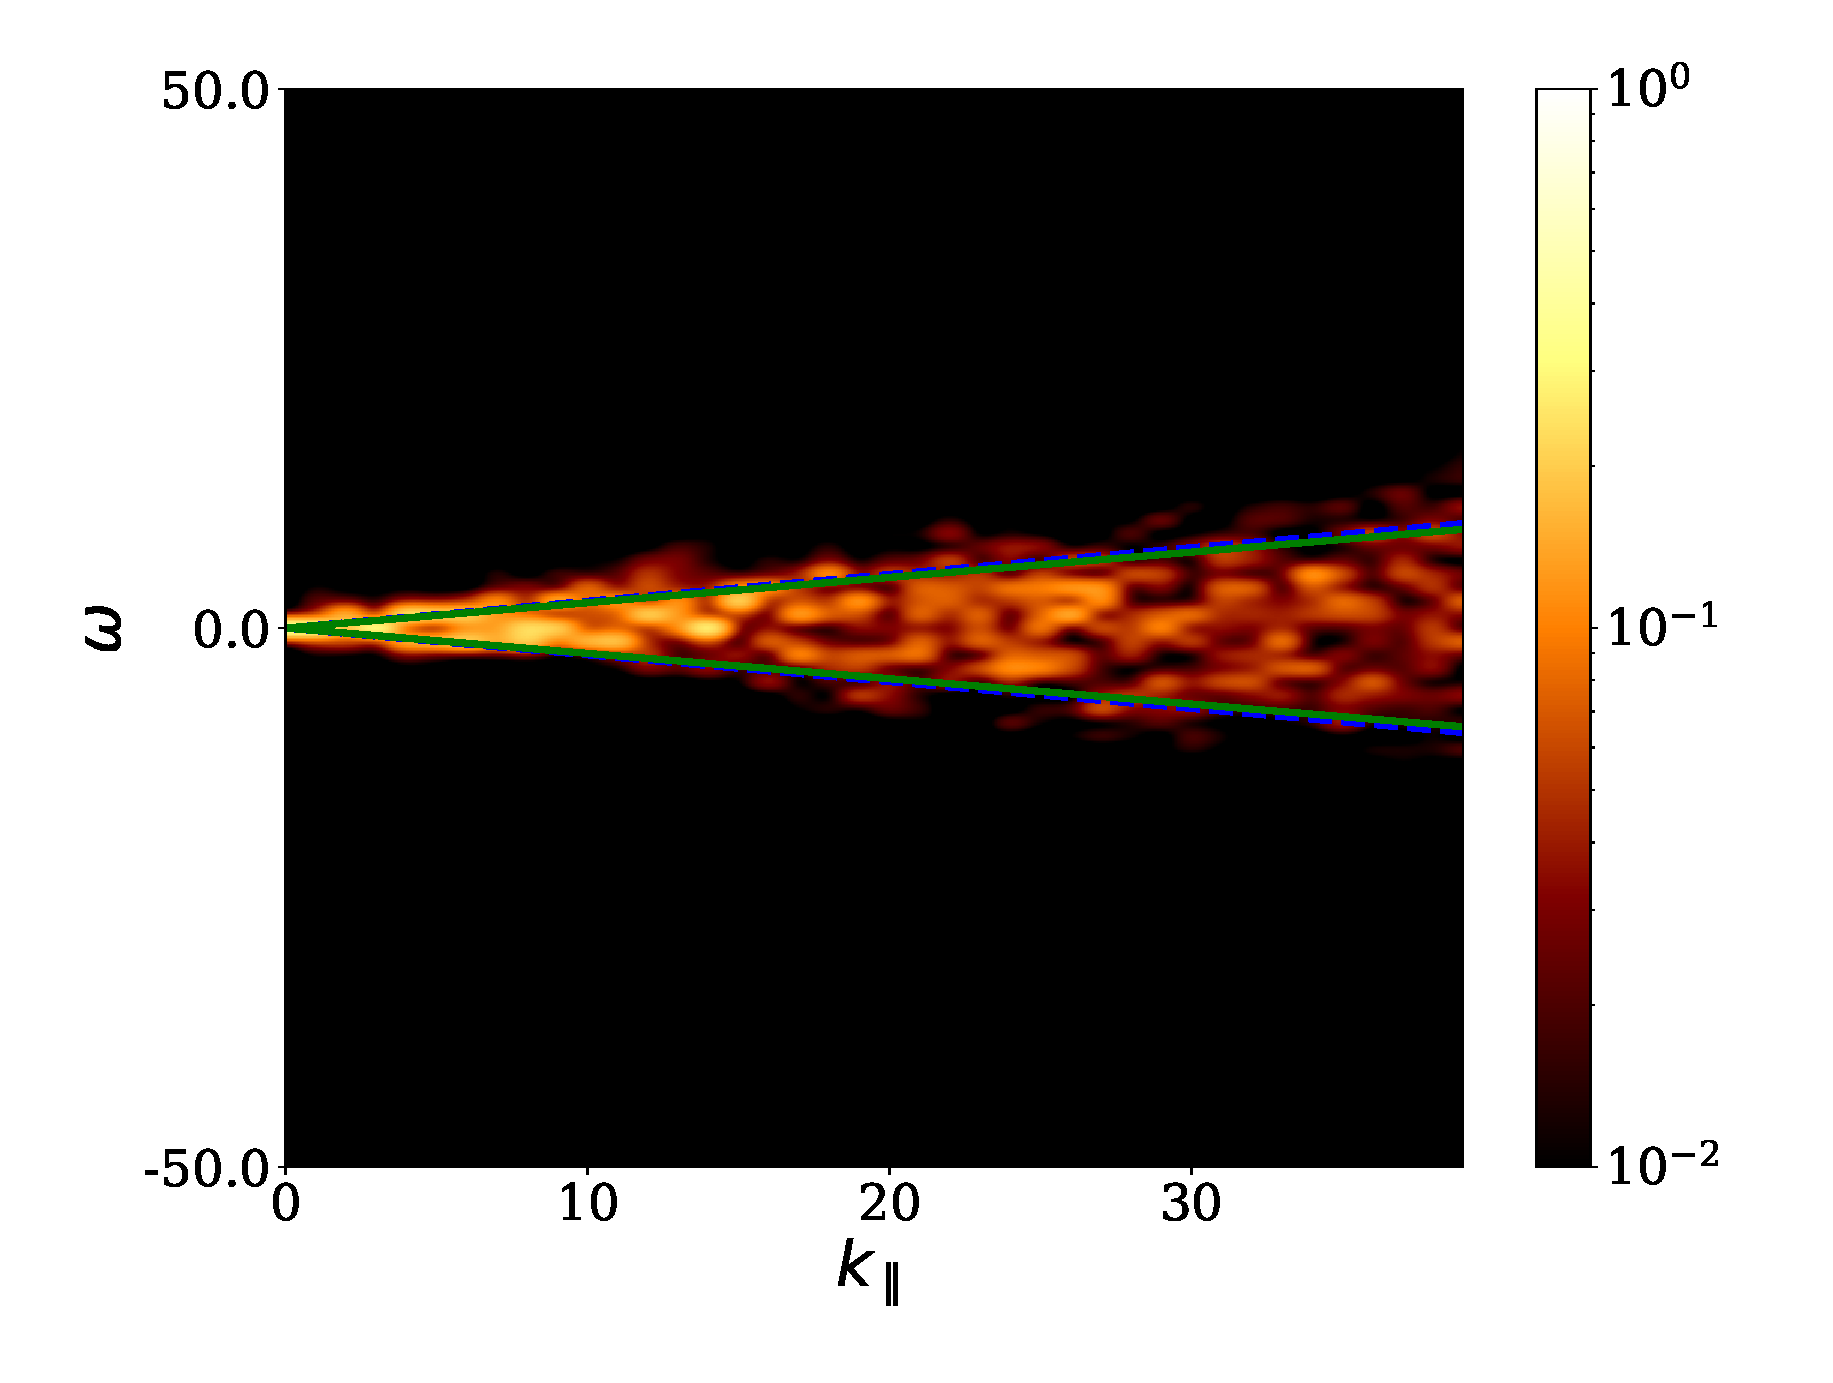
\includegraphics[width=0.95\textwidth]{{P2/fig3_B0.25_y_Hc0.0_zp_kperp0}.eps} \\
        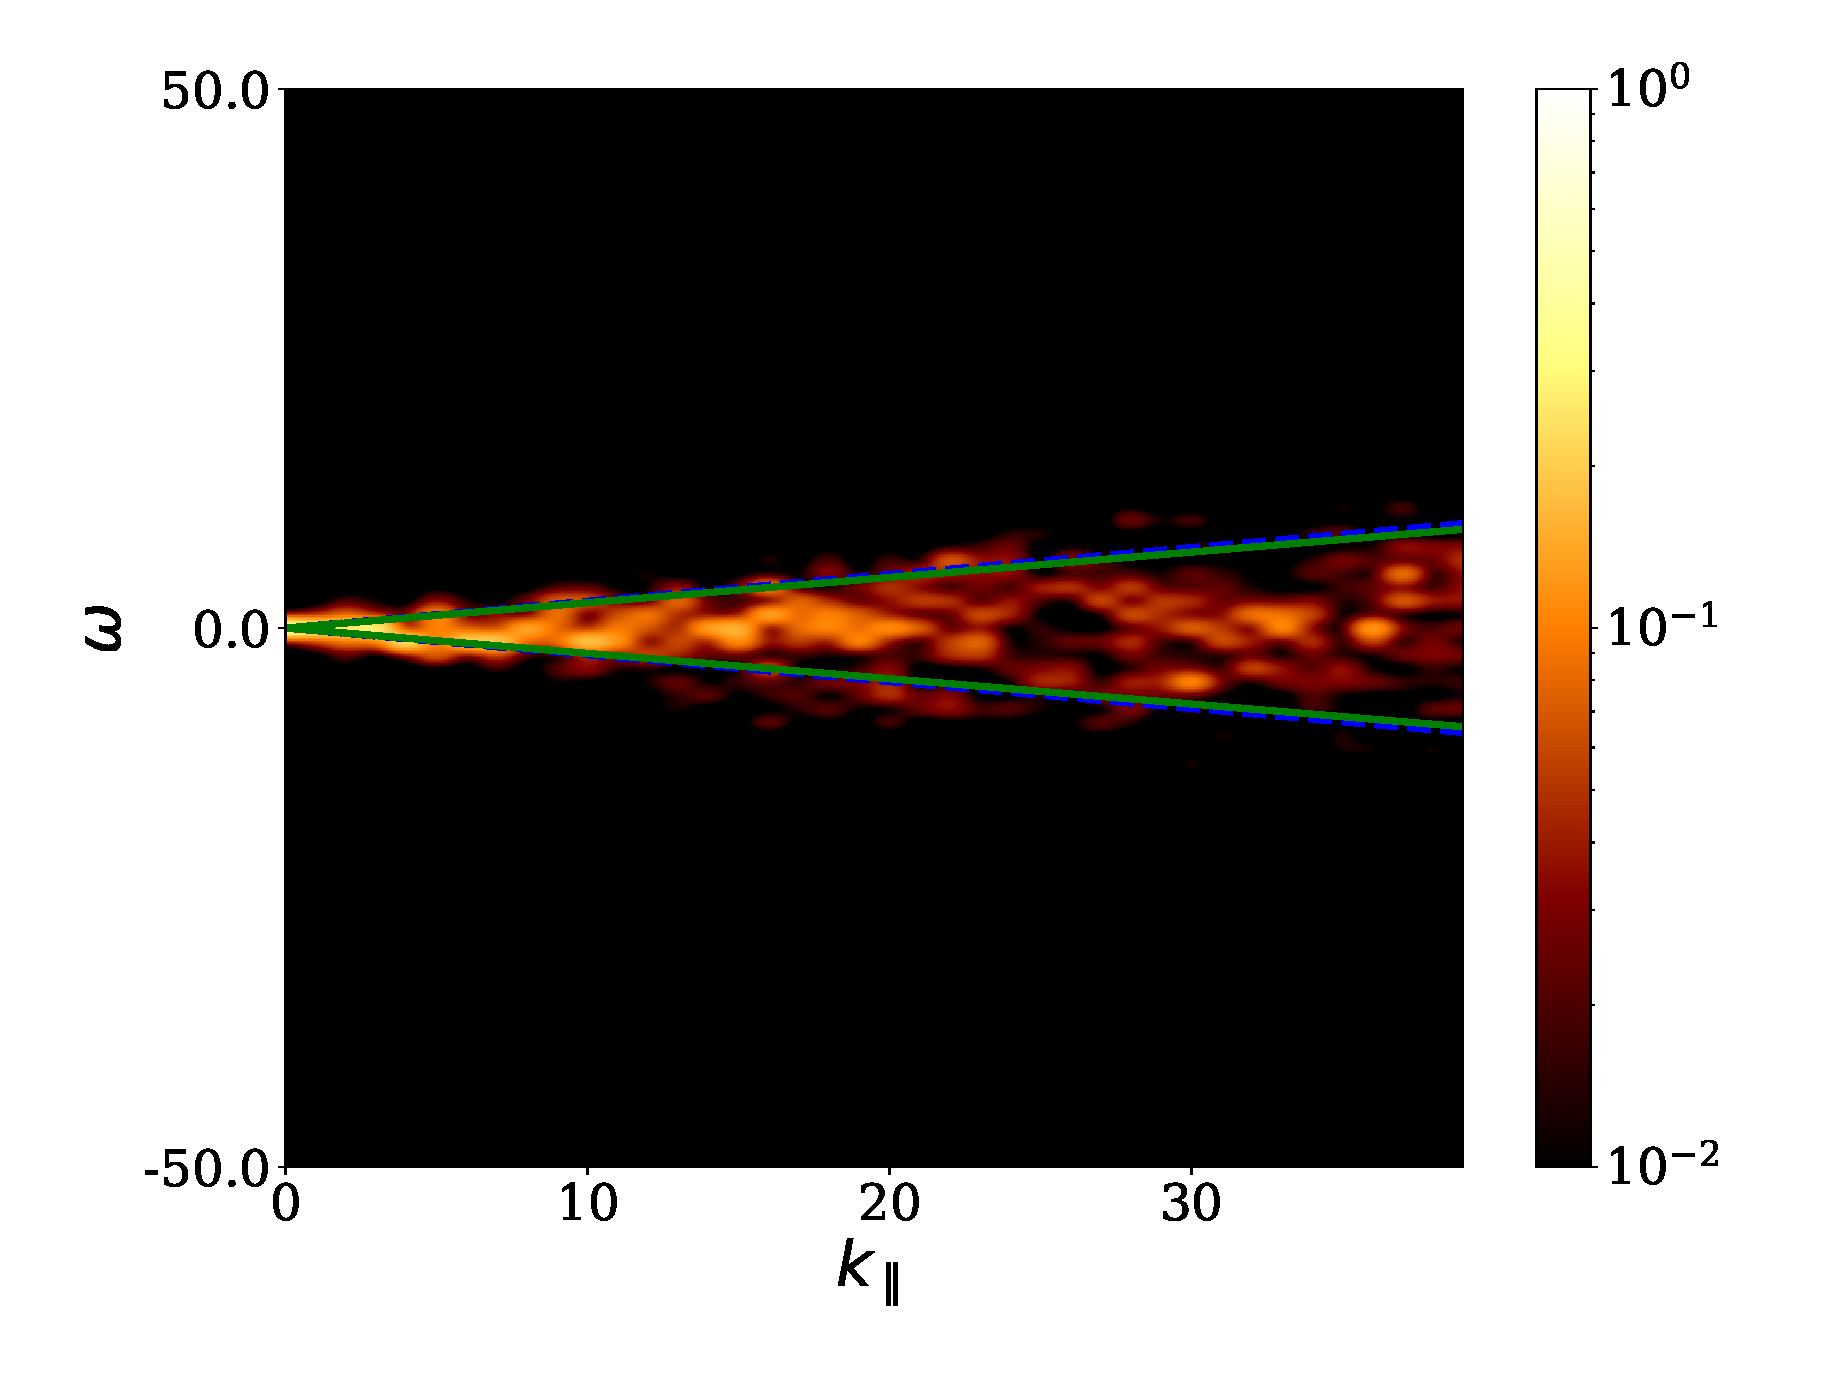
\includegraphics[width=0.95\textwidth]{{P2/fig3_B0.25_y_Hc0.0_zm_kperp0}.eps} \\
        {$\vec{z}^-$, $\sigma_c = 0.0$}
      \end{center}
    \end{minipage}
    \column{0.33\textwidth}
    \begin{minipage}[t]{1\textwidth}
      \begin{center}
        {$\vec{z}^+$, $\sigma_c = 0.3$} \\
        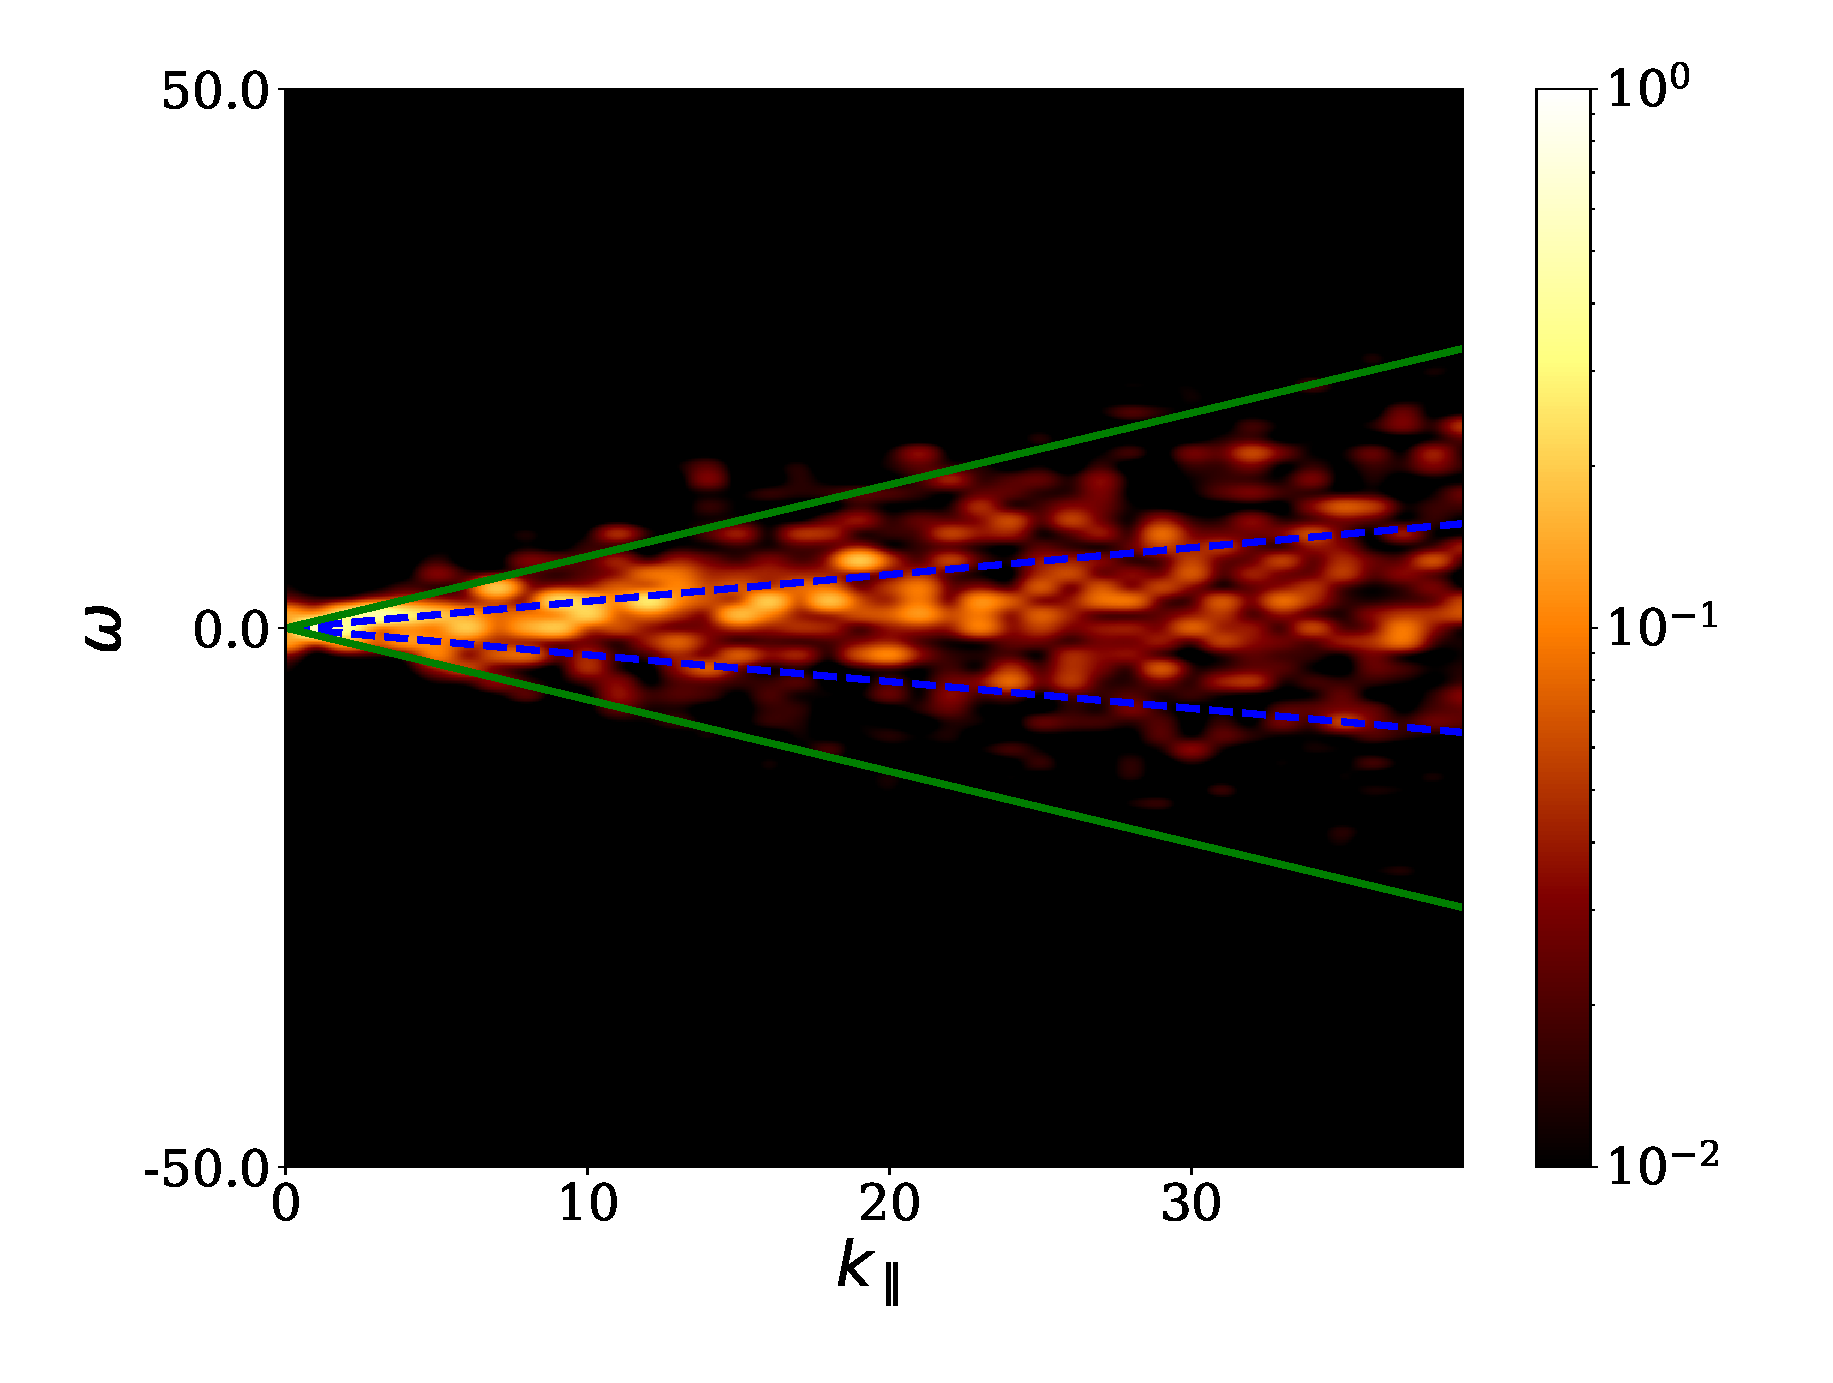
\includegraphics[width=0.95\textwidth]{{P2/fig3_B0.25_y_Hc0.3_zp_kperp0}.eps} \\
        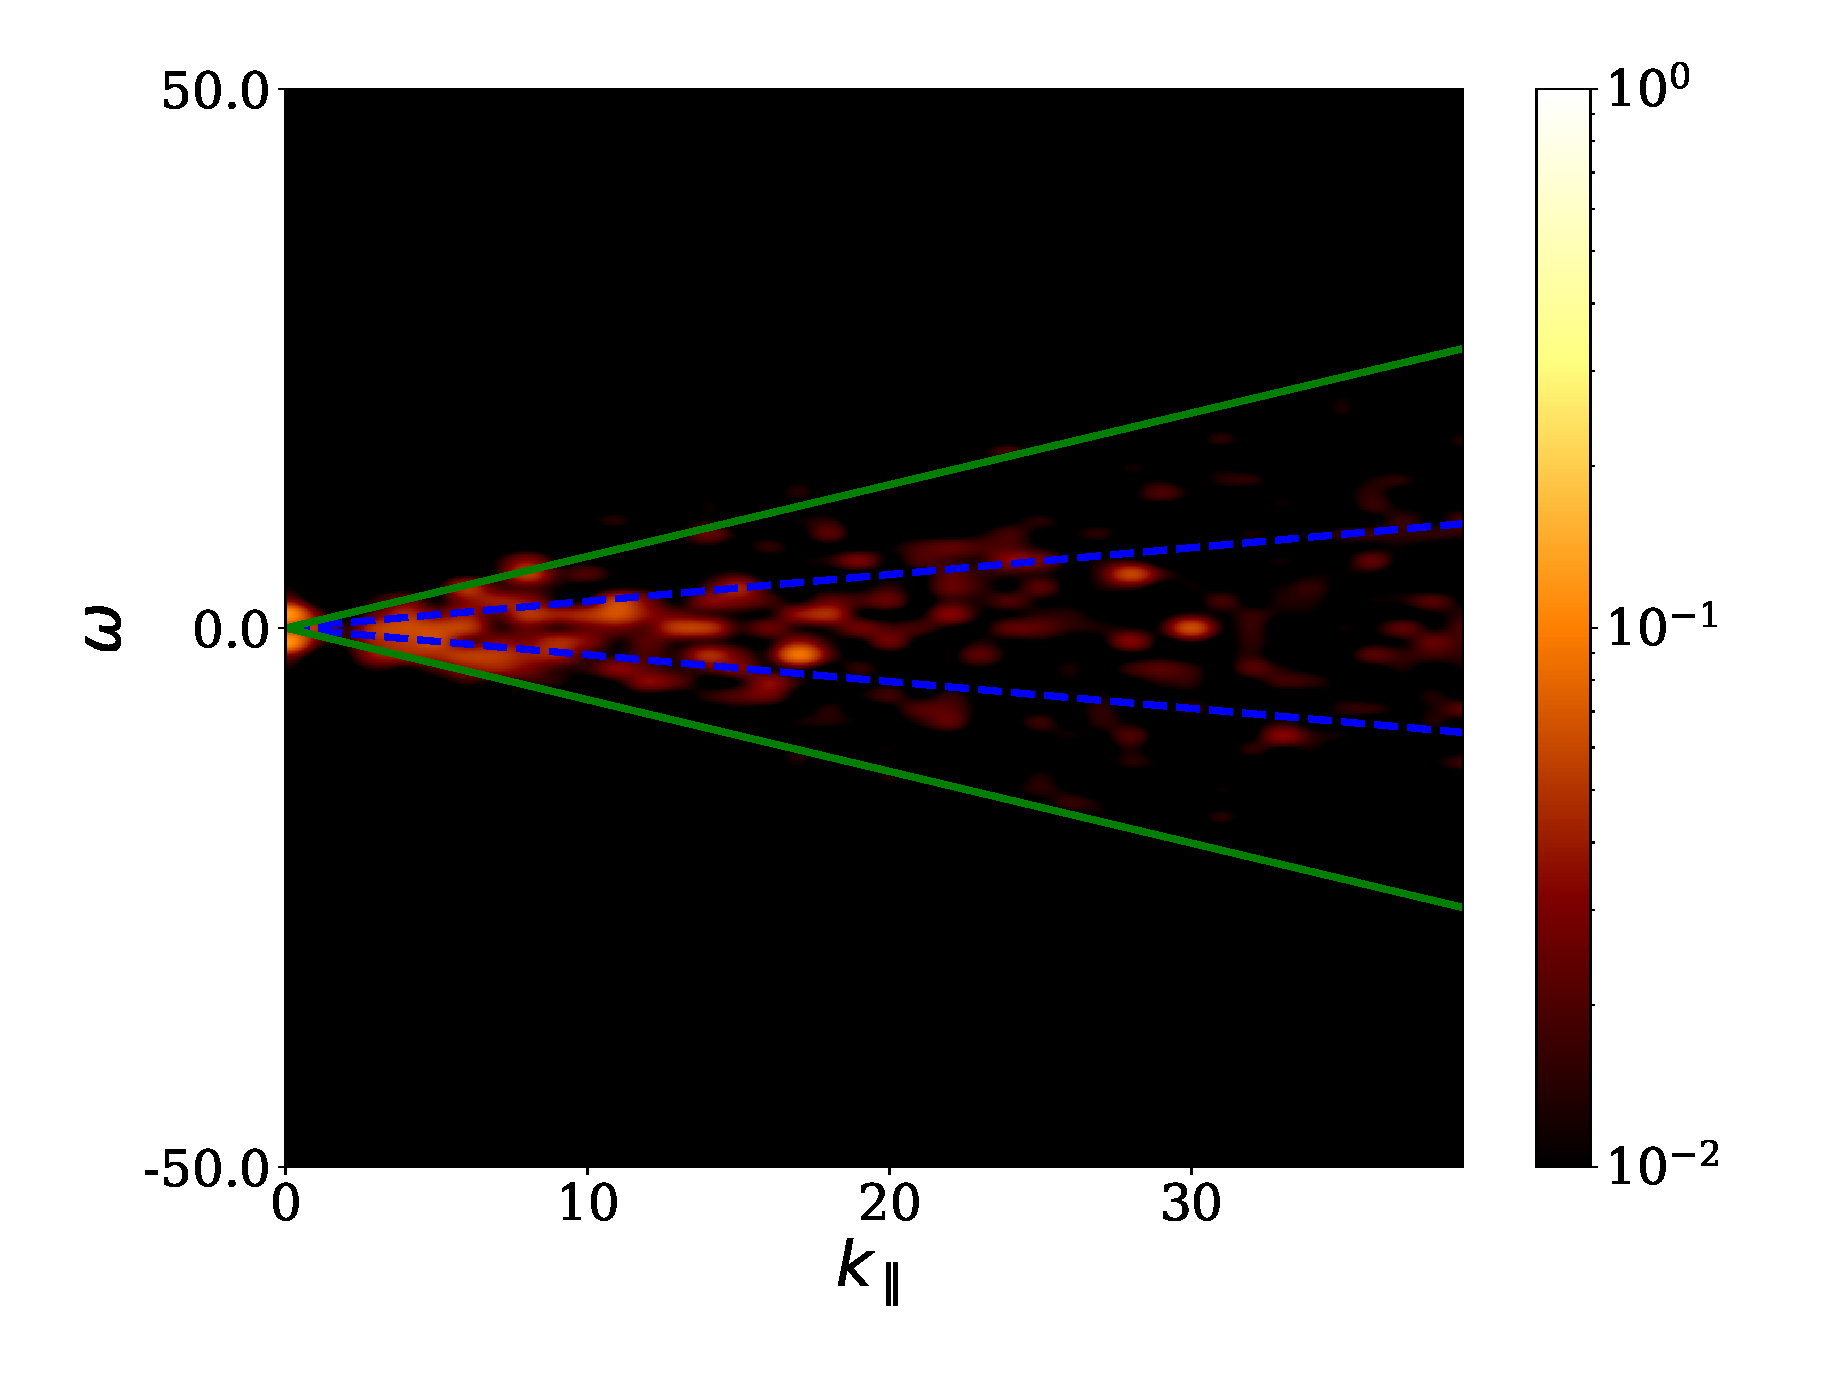
\includegraphics[width=0.95\textwidth]{{P2/fig3_B0.25_y_Hc0.3_zm_kperp0}.eps} \\
        {$\vec{z}^-$, $\sigma_c = 0.3$}
      \end{center}
    \end{minipage}
    \column{0.33\textwidth}
    \begin{minipage}[t]{1\textwidth}
      \begin{center}
        {$\vec{z}^+$, $\sigma_c = 0.9$} \\
        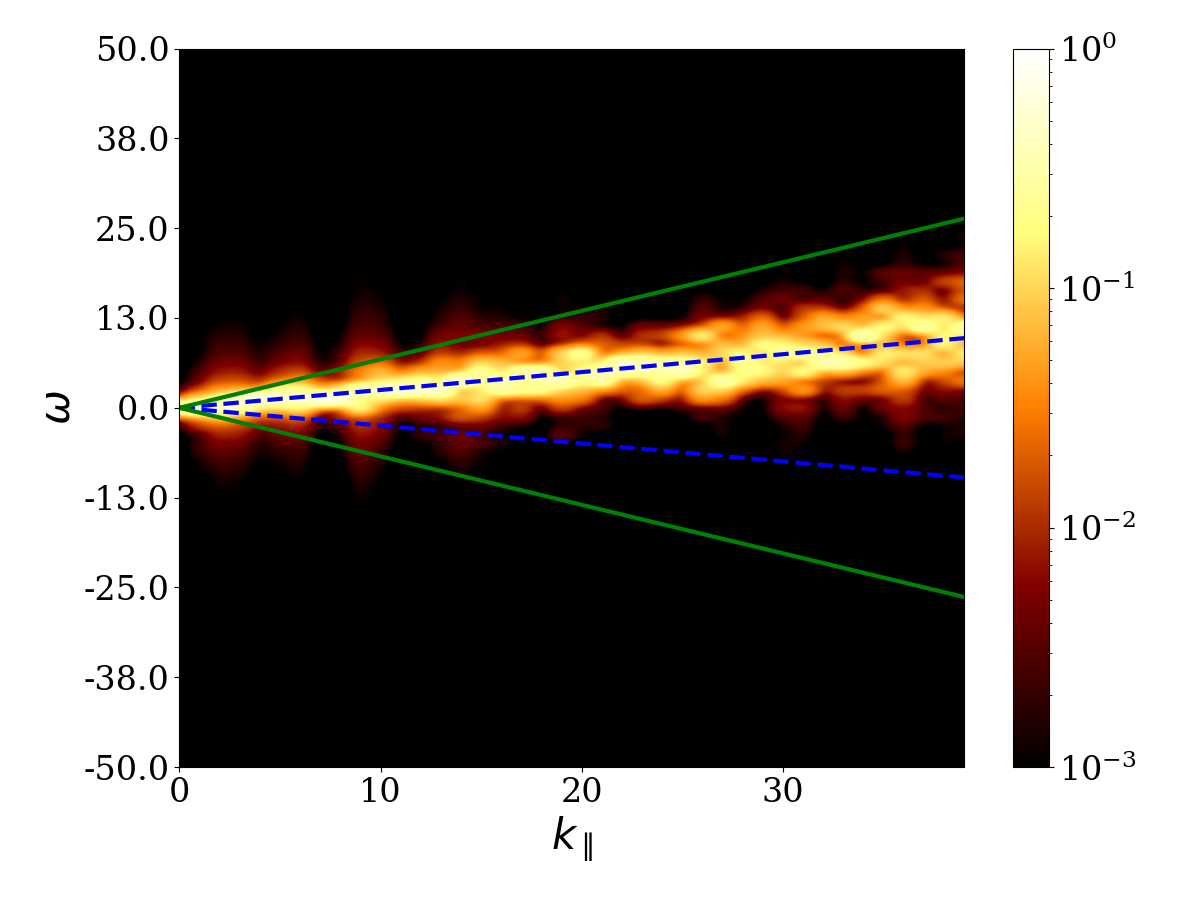
\includegraphics[width=0.95\textwidth]{{P2/fig3_B0.25_y_Hc0.9_zp_kperp0}.eps} \\
        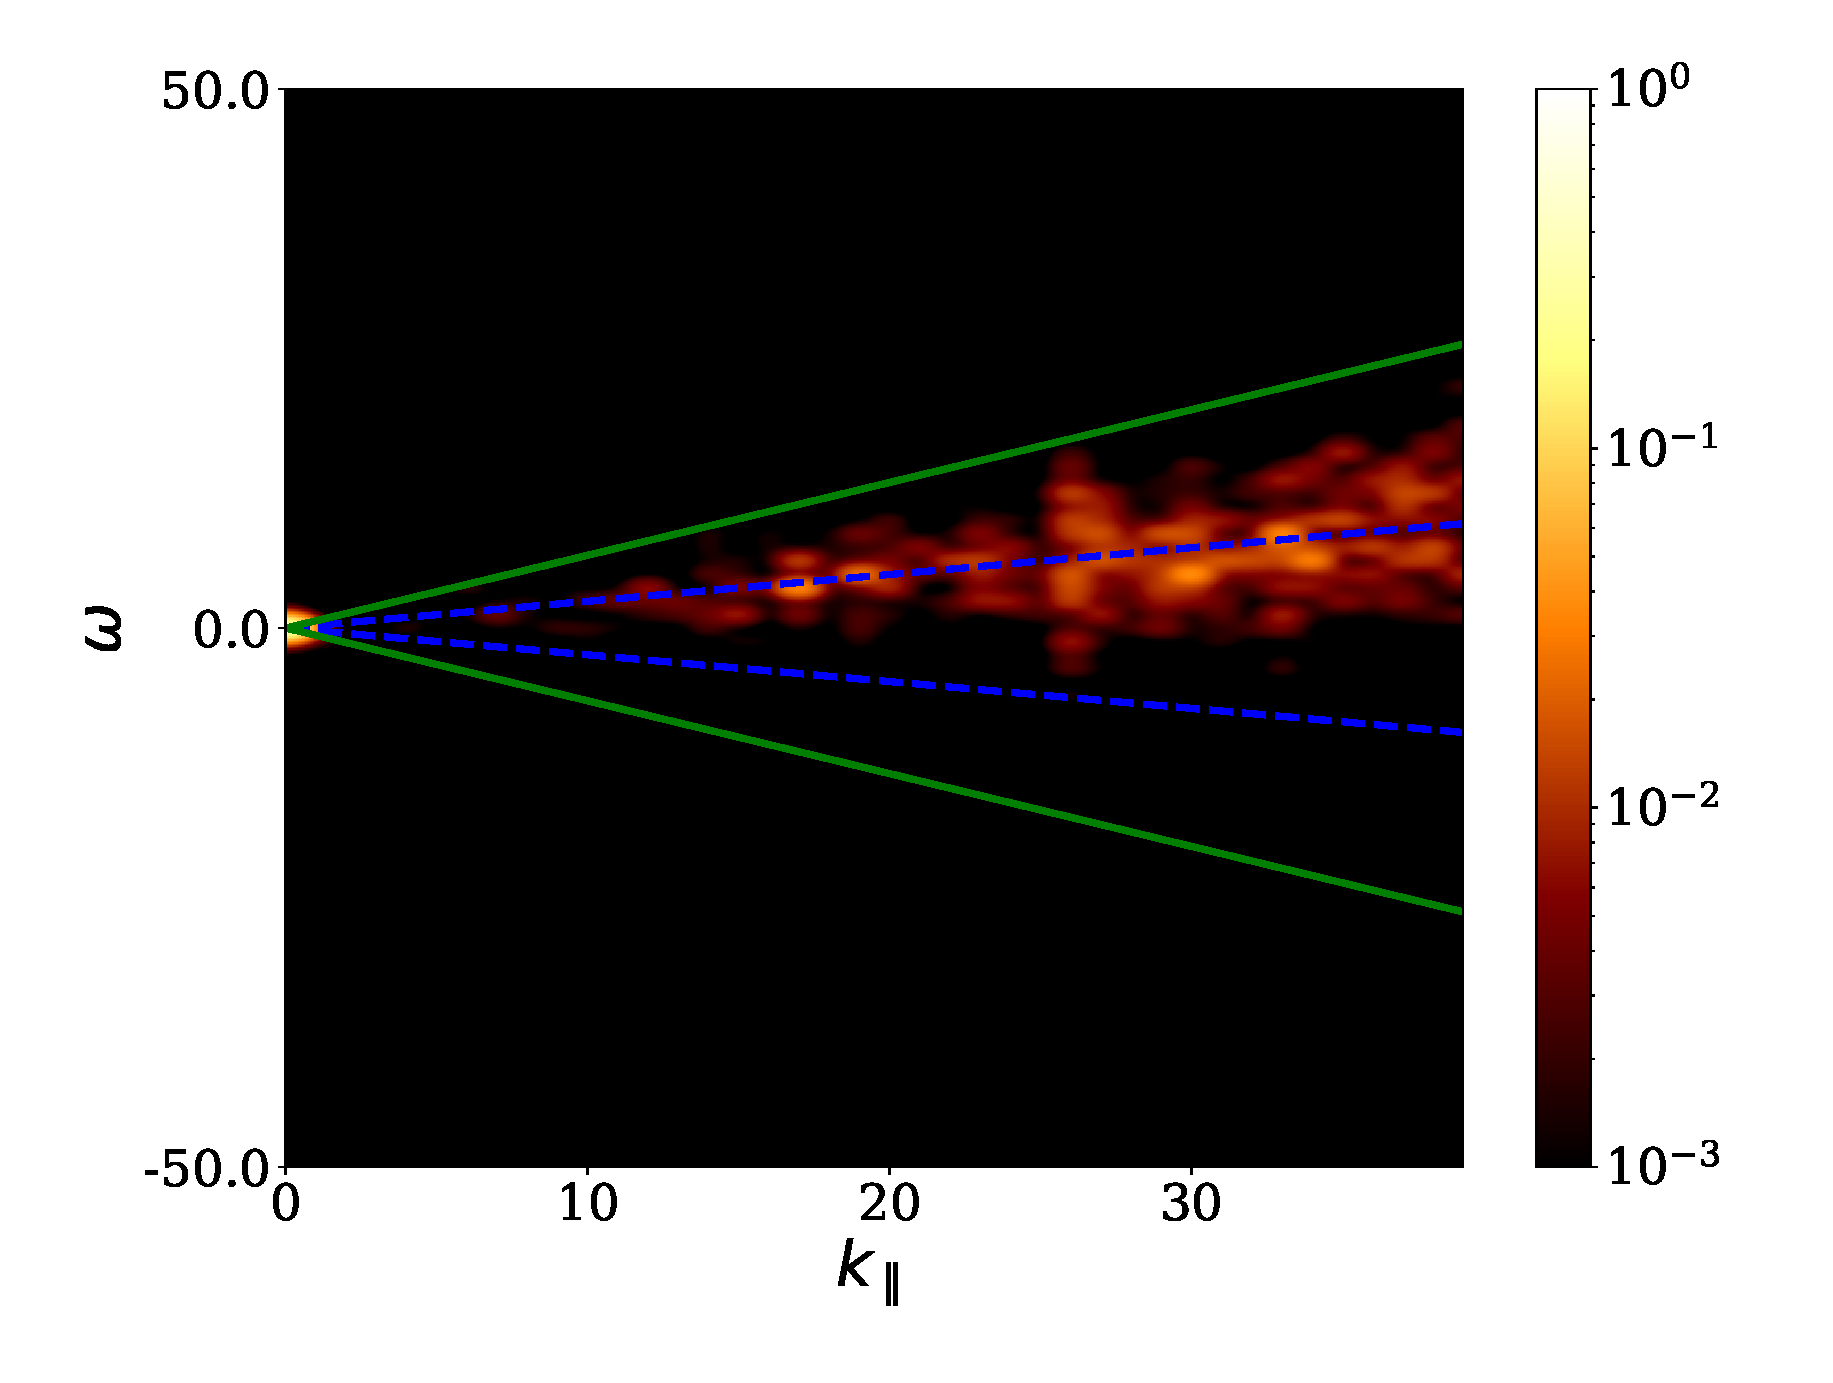
\includegraphics[width=0.95\textwidth]{{P2/fig3_B0.25_y_Hc0.9_zm_kperp0}.eps} \\
        {$\vec{z}^-$, $\sigma_c = 0.9$}
      \end{center}
    \end{minipage}
  \end{columns}
}
\note[itemize]{
\item Bajo $\sigma_c$, \textit{sweeping} dominante.
\item Energía en embudo de \emph{sweeping} para $\sigma_c$ bajo;
  energía en Alfvén para $\sigma_c$ alto.
\item Con $\sigma_c$ alto, más energía en $\vec{z}^+$.
\item Las fluctuaciones $\vec{z}^+$ se propagan antiparalelamente al
  campo guía, como es esperado. Pero las $\vec{z}^-$ también
  (contradicción?).
}





\frame{\frametitle{Espectros espacio-temporales}
  {\large \underline{Espectro energético normalizado $E({\bf k}, \omega)/E({\bf k})$}}
  {\large, $B_0 = 8$}\vspace{10pt}
  \begin{columns}
    \column{0.33\textwidth}
    \begin{minipage}[t]{1\textwidth}
      \begin{center}
        {$\vec{z}^+$, $\sigma_c = 0.0$} \\
        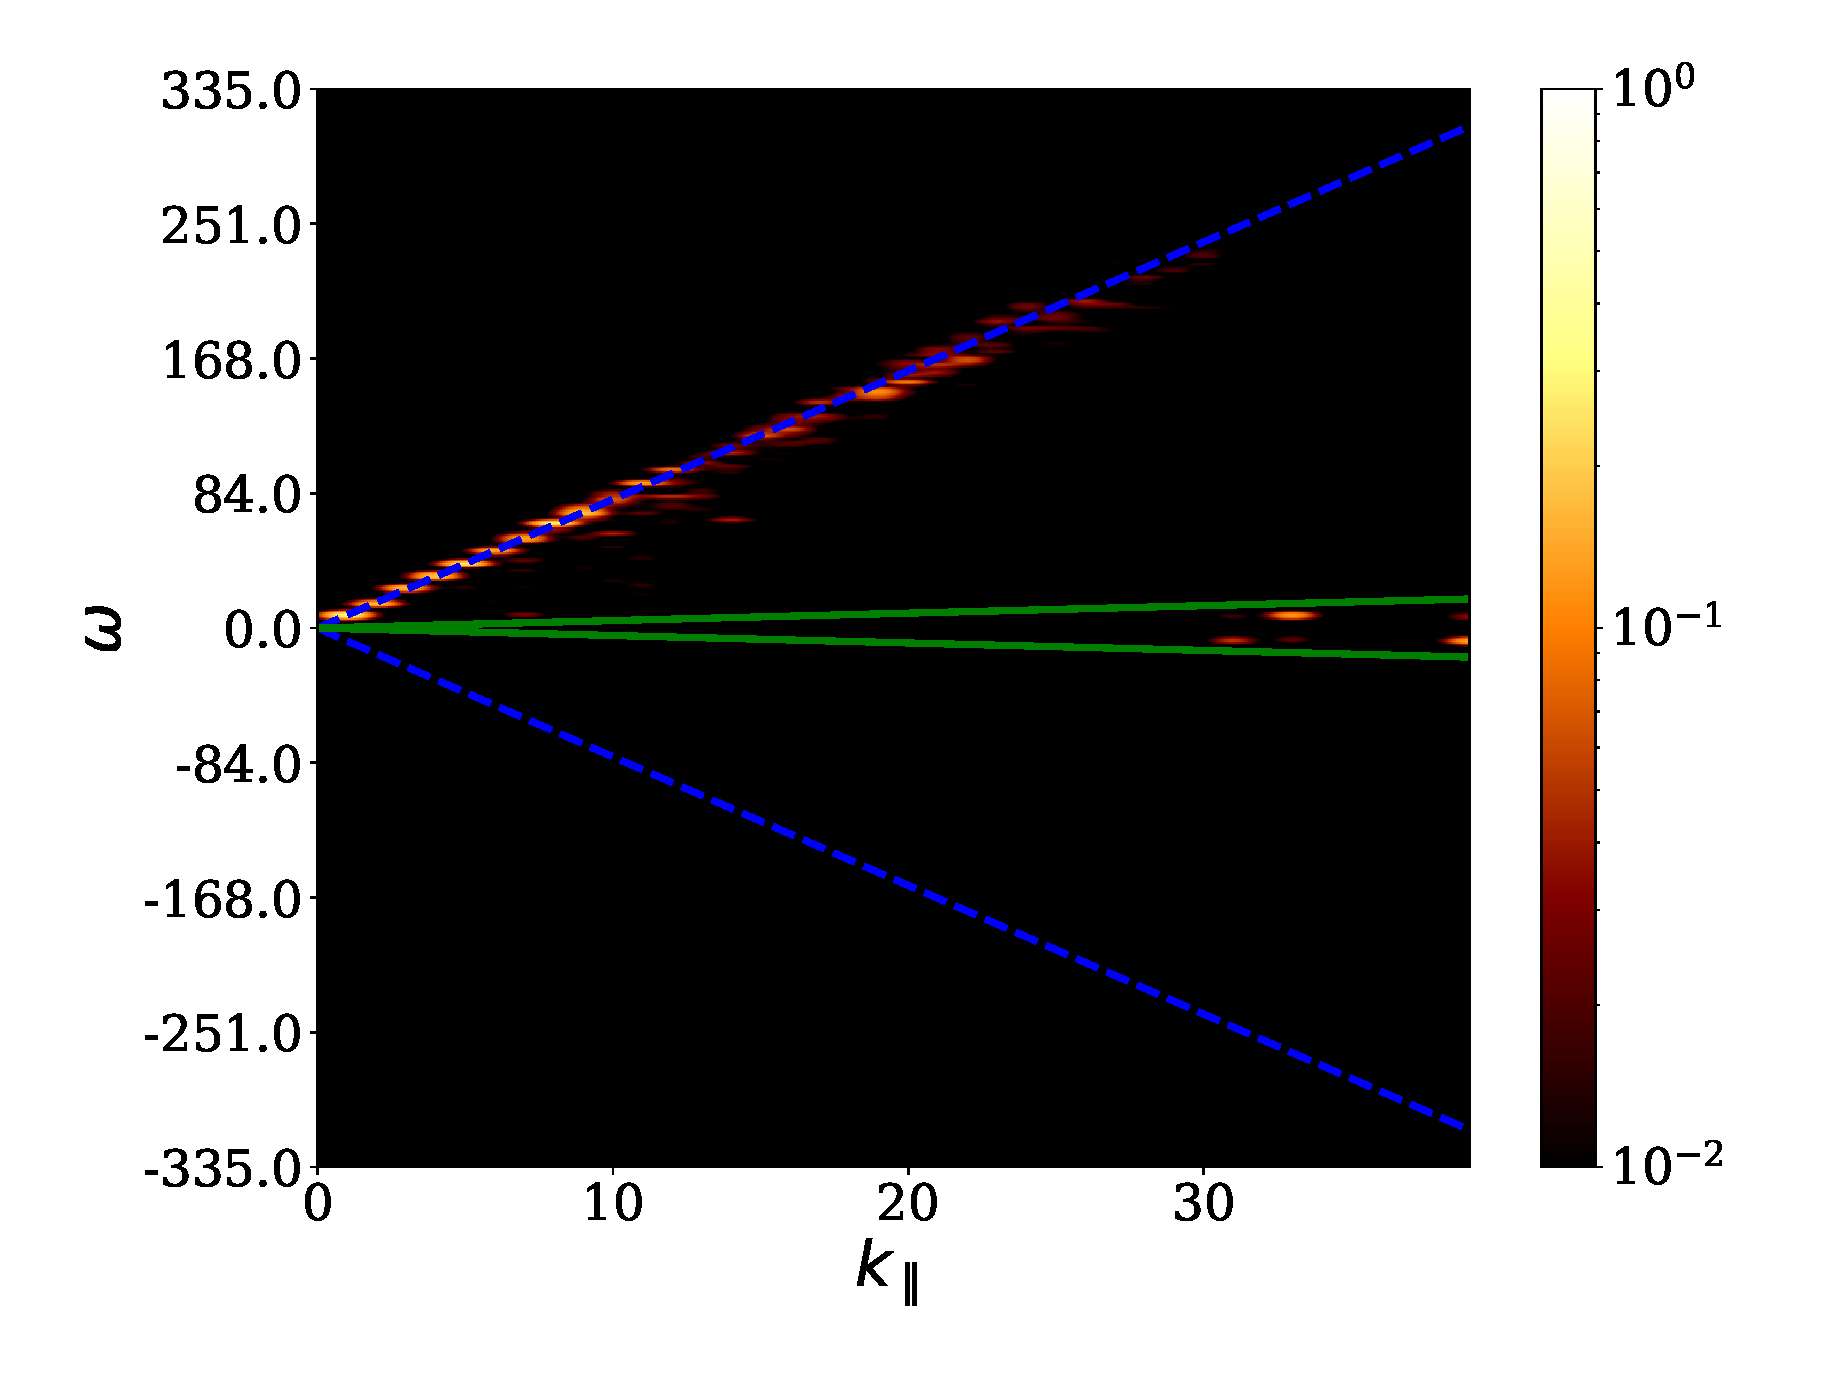
\includegraphics[width=0.95\textwidth]{{P2/fig3_B8.0_y_Hc0.0_zp_kperp0}.eps} \\
        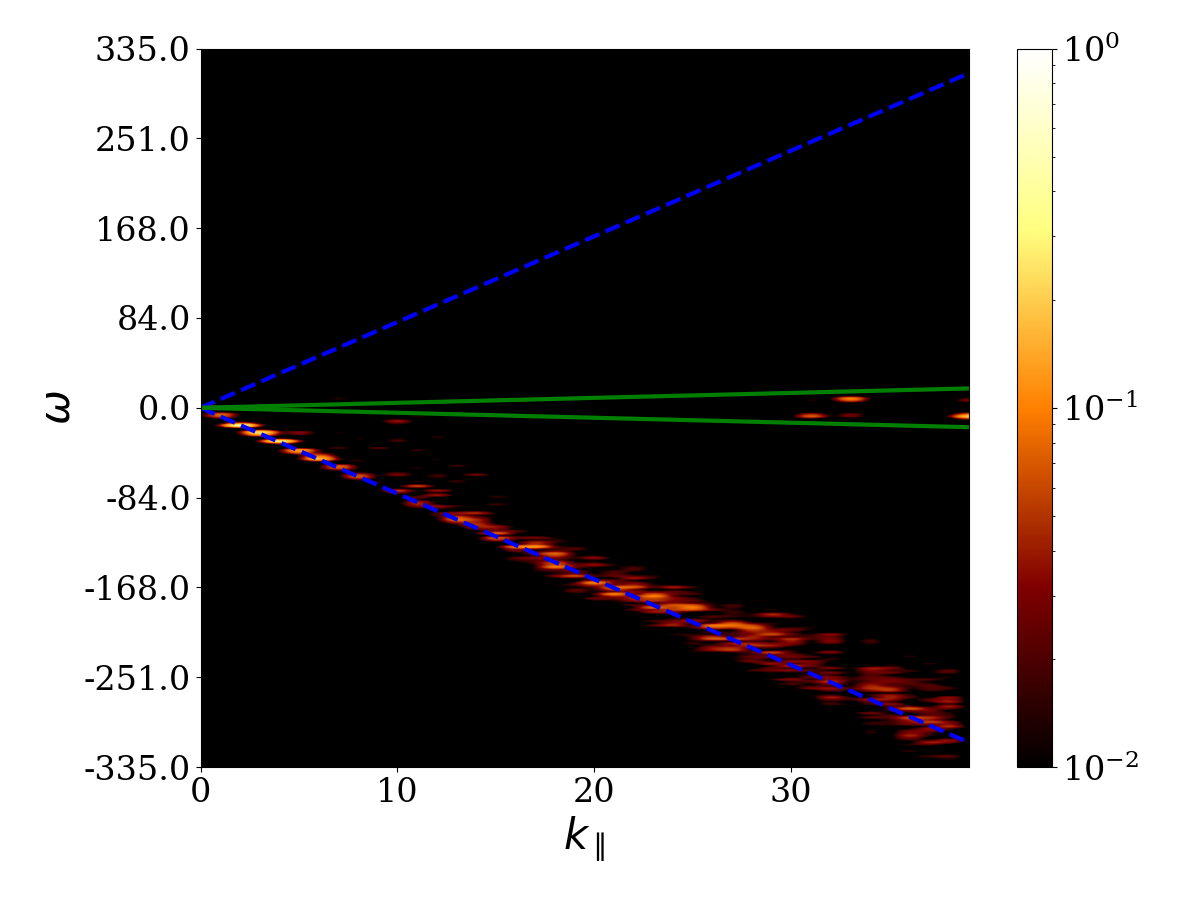
\includegraphics[width=0.95\textwidth]{{P2/fig3_B8.0_y_Hc0.0_zm_kperp0}.eps} \\
        {$\vec{z}^-$, $\sigma_c = 0.0$}
      \end{center}
    \end{minipage}
    \column{0.33\textwidth}
    \begin{minipage}[t]{1\textwidth}
      \begin{center}
        {$\vec{z}^+$, $\sigma_c = 0.3$} \\
        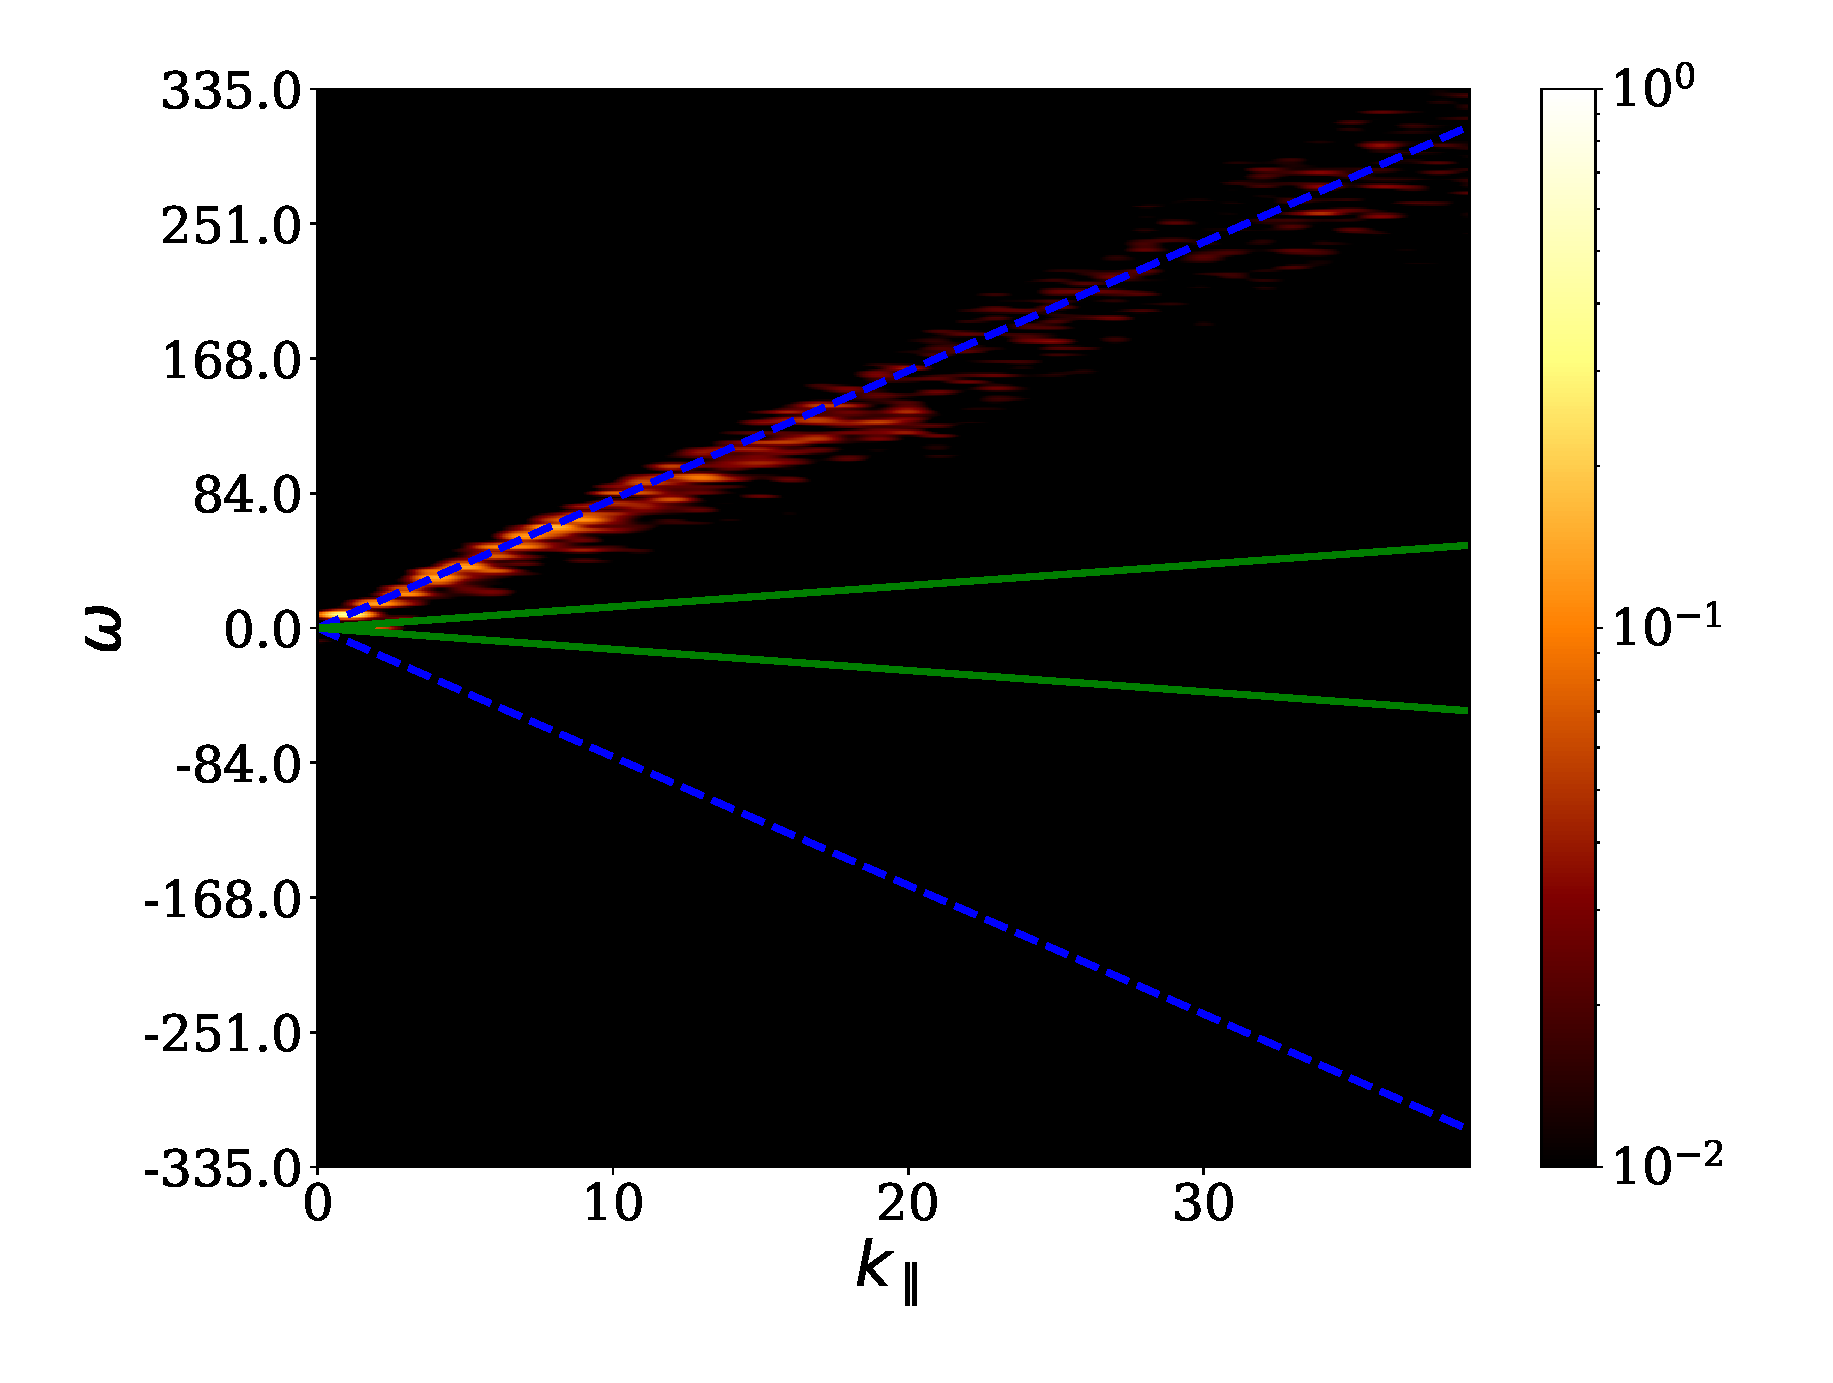
\includegraphics[width=0.95\textwidth]{{P2/fig3_B8.0_y_Hc0.3_zp_kperp0}.eps} \\
        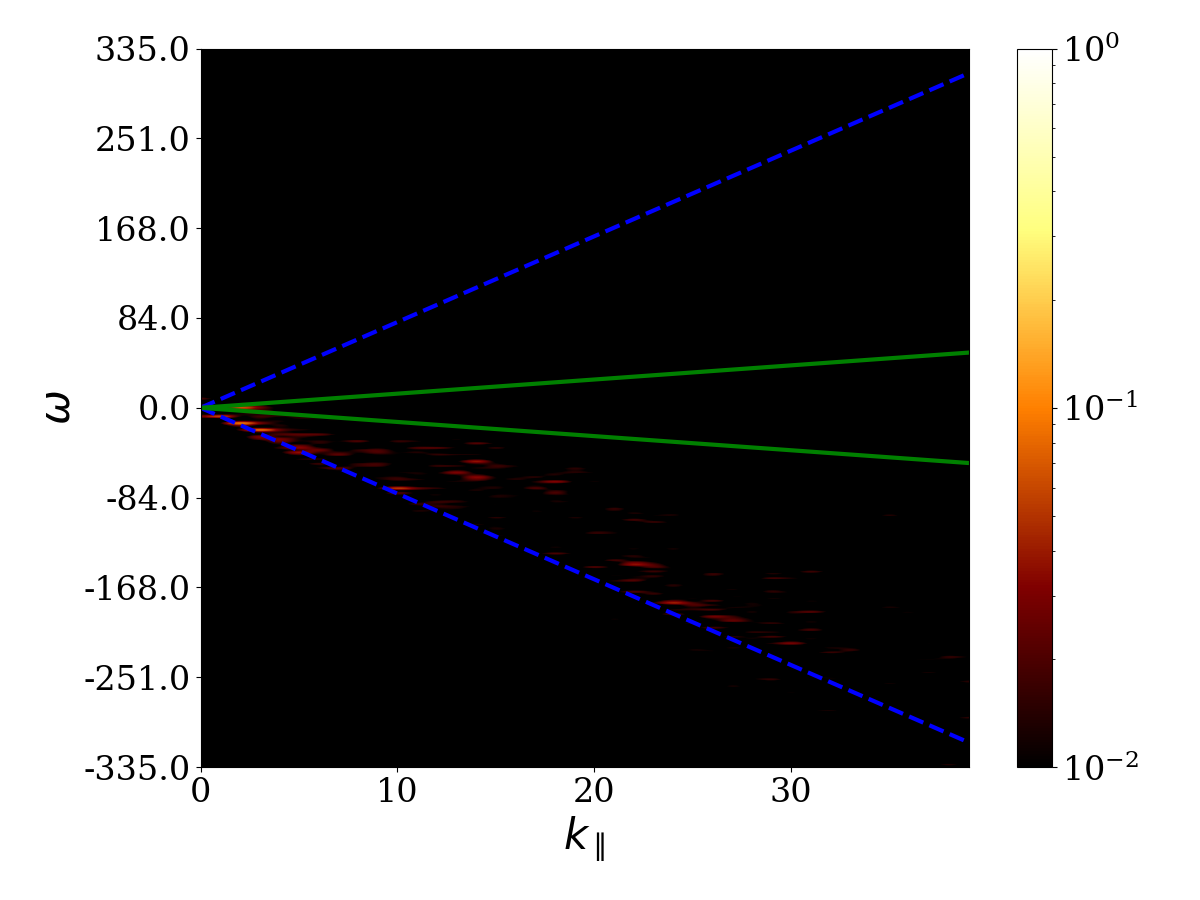
\includegraphics[width=0.95\textwidth]{{P2/fig3_B8.0_y_Hc0.3_zm_kperp0}.eps} \\
        {$\vec{z}^-$, $\sigma_c = 0.3$}
      \end{center}
    \end{minipage}
    \column{0.33\textwidth}
    \begin{minipage}[t]{1\textwidth}
      \begin{center}
        {$\vec{z}^+$, $\sigma_c = 0.9$} \\
        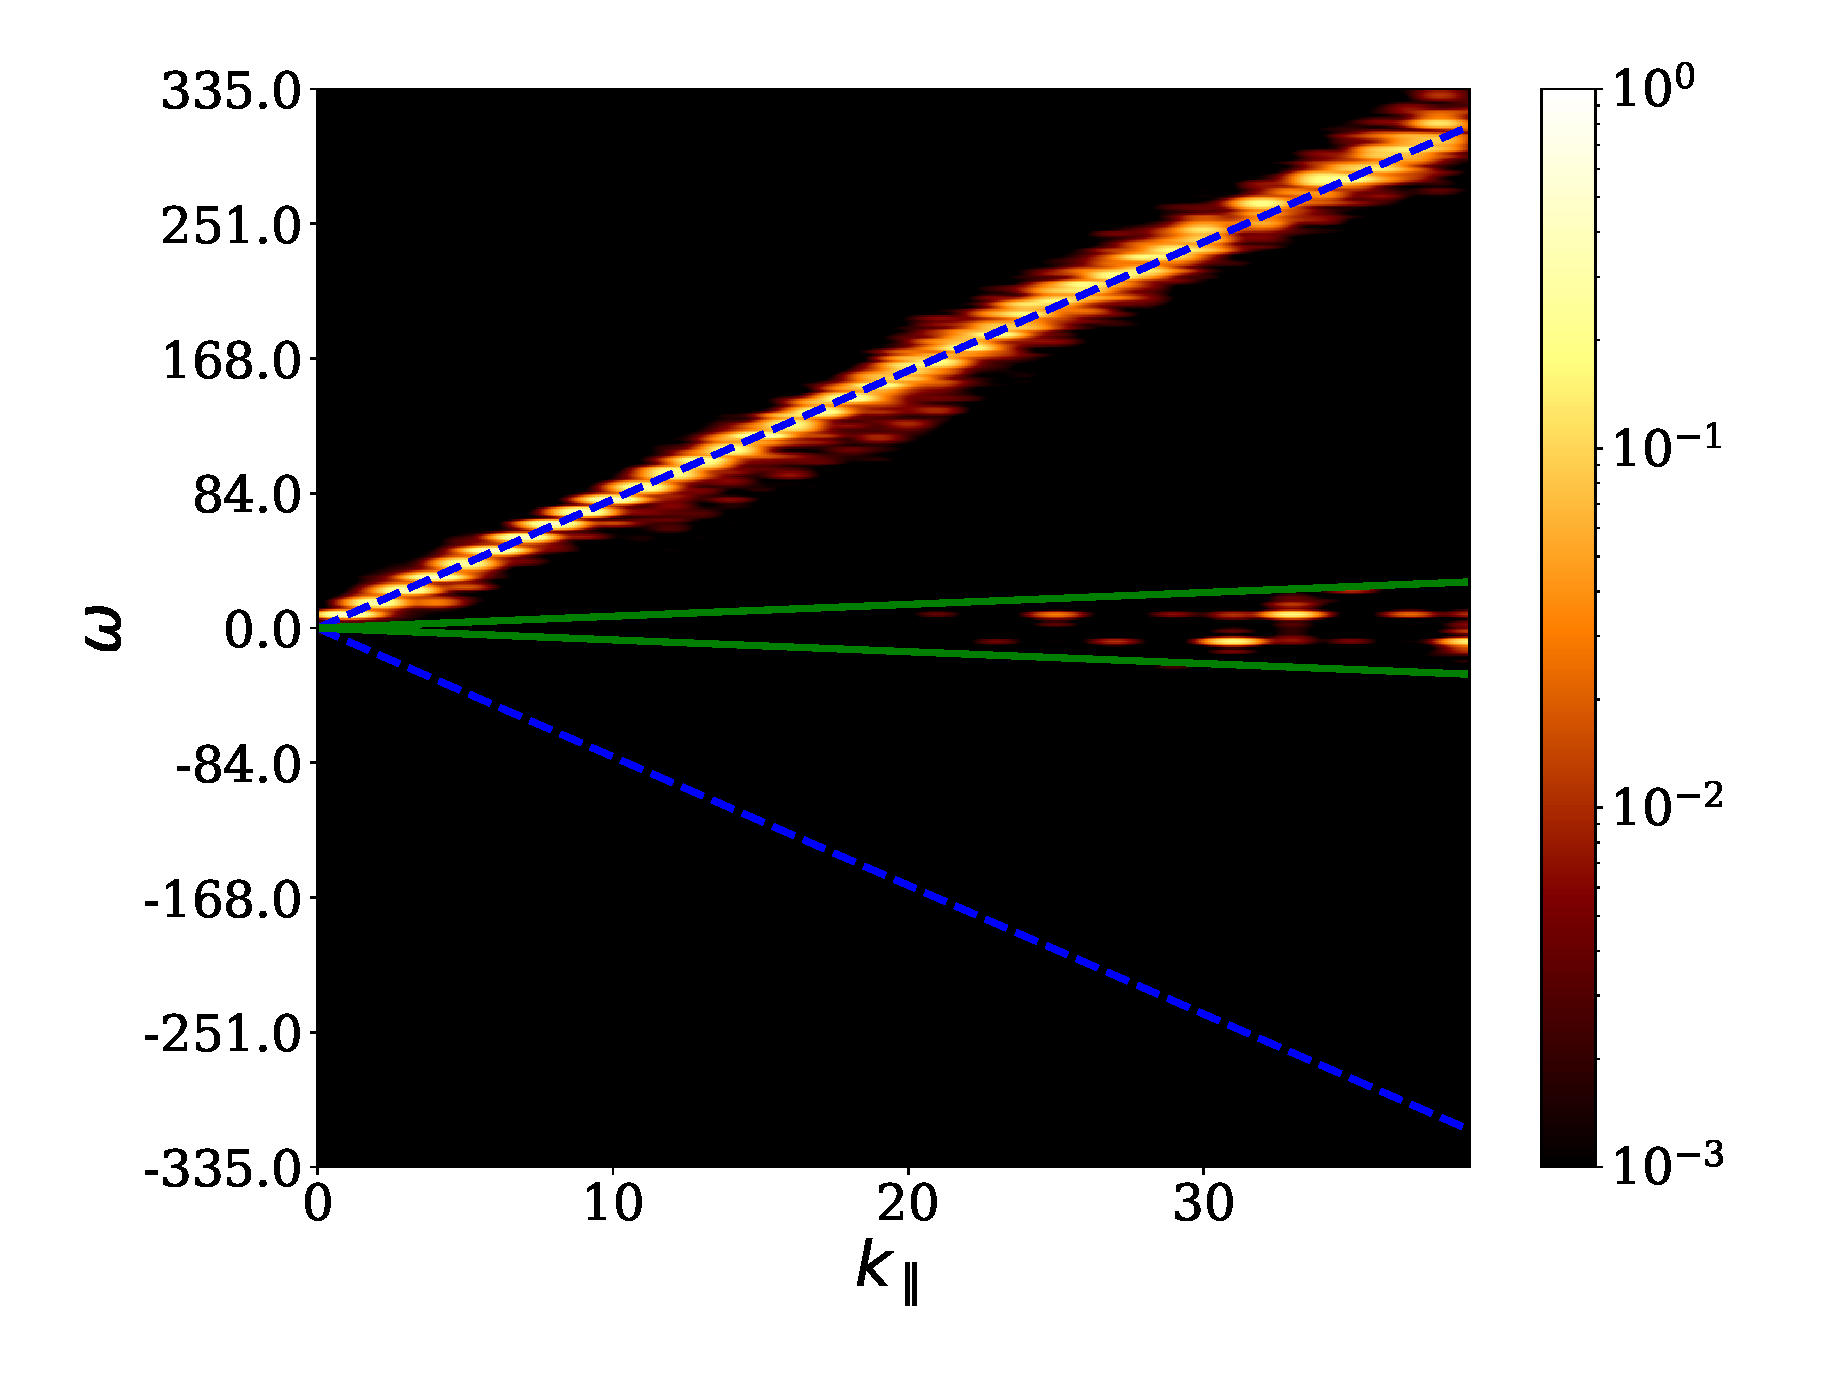
\includegraphics[width=0.95\textwidth]{{P2/fig3_B8.0_y_Hc0.9_zp_kperp0}.eps} \\
        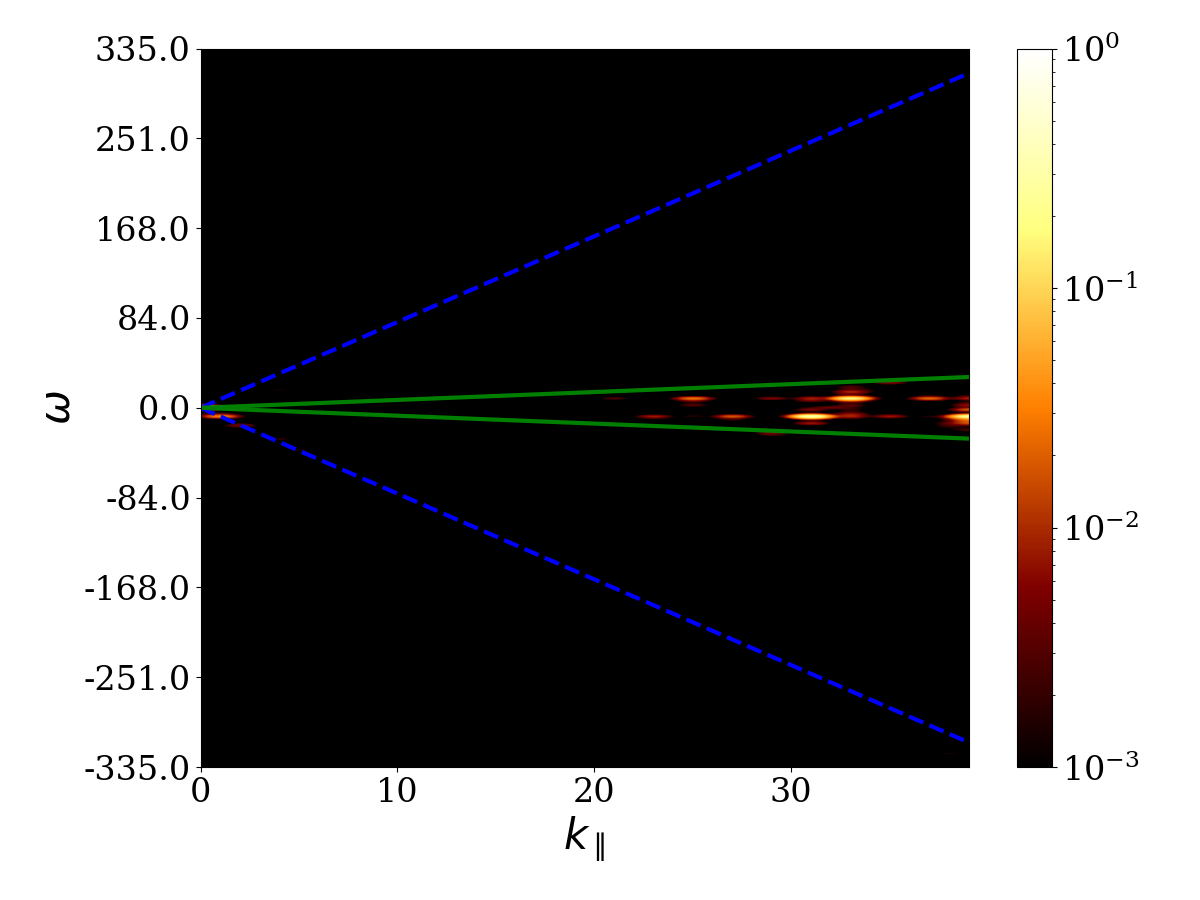
\includegraphics[width=0.95\textwidth]{{P2/fig3_B8.0_y_Hc0.9_zm_kperp0}.eps} \\
        {$\vec{z}^-$, $\sigma_c = 0.9$}
      \end{center}
    \end{minipage}
  \end{columns}
}
\note[itemize]{
\item En todos los
  casos, la energía se concentra en una región angosta cerca de la
  relación de dispersión de las ondas, $\omega^\pm \approx \pm
  \vec{V}_A\cdot\vec{k}$, o cerca de $\omega \approx 0$, para
  todos los números de onda estudiados.
\item No hay evidencia de contrapropagación de ondas.
}



\frame{\frametitle{Espectros espacio-temporales: contrapropagación de ondas}
  ?`A qué se debe está propagación antiparalela al campo guía de
  $\vec{z}^-$ en algunos casos?
  \pause
  \begin{itemize}
  \item Comportamiento predicho por Hollweg (1990) para el viento
    solar.
  \item Es causado, por ejemplo, por reflexiones de ondas debido a
    fluctuaciones de la densidad en el medio interplanetario,
    utilizando la expansión WKB.
  \item Pero en nuestro caso, el flujo es incompresible y la densidad
    es uniforme en el espacio y constante en el tiempo. ?`Entonces?
  \end{itemize}
}
\note[itemize]{
\item Como en óptica, cuando el índice de refracción cambia, pueden darse reflexiones
}




\frame{\frametitle{Espectros espacio-temporales: contrapropagación de ondas}
  Cualitativamente, se debe a reflexiones en inhomogeneidades de
  gran escala del campo magnético medio (no hay un flujo
  medio de fondo, ni fluctuaciones de
  densidad).\vfill

  \begin{center}
  $\vec{B} = \vec{B_0} + \vec{B_{\text{k bajos}}} + \vec{b_{\text{k altos}}}$
  \end{center}\vfill
  
  Como resultado, el flujo tiene una velocidad de Alfvén
  efectiva que depende de las coordenadas espaciales.\vfill

  Así, este último argumento cualitativo indica (en acuerdo con las
  simulaciones) que las fluctuaciones $\vec{z}^-$ pueden propagarse
  con la misma velocidad de fase y dirección que las fluctuaciones
  $\vec{z}^+$, siempre que $\sigma_c \neq 0$ y $B_0$ no sea demasiado
  fuerte para un valor fijado de la helicidad cruzada normalizada.
}
\note[itemize]{
\item El campo magnético total tiene una parte uniforme, pero también una
  componente fluctuante lentamente variable (por ejemplo, los modos
  con $k=1$, que evolucionan en una escala temporal más lenta que las
  ondas rápidas y las fluctuaciones de pequeñas escalas).
  \item La demostración no es obvia, es necesario hacer la cuenta. Está en la tesis y en un anexo.
}


\frame{\frametitle{Espectros espacio-temporales: contrapropagación de ondas}
En otras palabras, si $|\vec{z}^+|$ a grandes escalas es comparable
  con $|\vec{V}_{A}|$ y $\sigma_c \approx 1$, podemos ver que
  las fluctuaciones $\vec{z}^-$ se propagan en la misma dirección que
  las fluctuaciones $\vec{z}^+$ como resultado de reflexiones en
  inhomogeneidades del campo magnético de gran escala.\vfill

  Un comportamiento similar puede resultar, por ejemplo, a partir de
  fluctuaciones en la densidad de masa cuando el fluido es
  compresible.\vfill

  Cuando la intensidad del campo magnético de fondo se aumenta aún
  más, los argumentos utilizados dejan de ser válidos, y la relevancia
  de las reflexiones se reduce (caso con $B_0=8$).
}
\note[itemize]{
\item 2) ... como es el caso de algunas regiones del viendo solar y
  en el medio interplanetario, y este argumento no imposibilita a
  otros efectos (tales como interacciones fuertes no lineales) de
  resultar en reflexiones y contrapropagaciones de las
  excitaciones.
}



\frame{\frametitle{Tiempos de descorrelación}
Nuevamente, apoyamos los resultados anteriores estudiando el tiempo de
descorrelación $\tau_D$, y comparándolo con los tiempos teóricos
pertinentes.
}


\frame{\frametitle{Tiempos de descorrelación}
  {\large \underline{$\vec{z}^+$ vs $\vec{z}^-$}} - Casos con $B_0 = 1$, $\sigma_c = 0.3$, $k_\parallel = 10$ \vspace{10pt}
  \begin{columns}
    \column{0.5\textwidth}
    \begin{minipage}[t]{1\textwidth}
      \begin{center}
        {$\vec{z}^-$} \\
        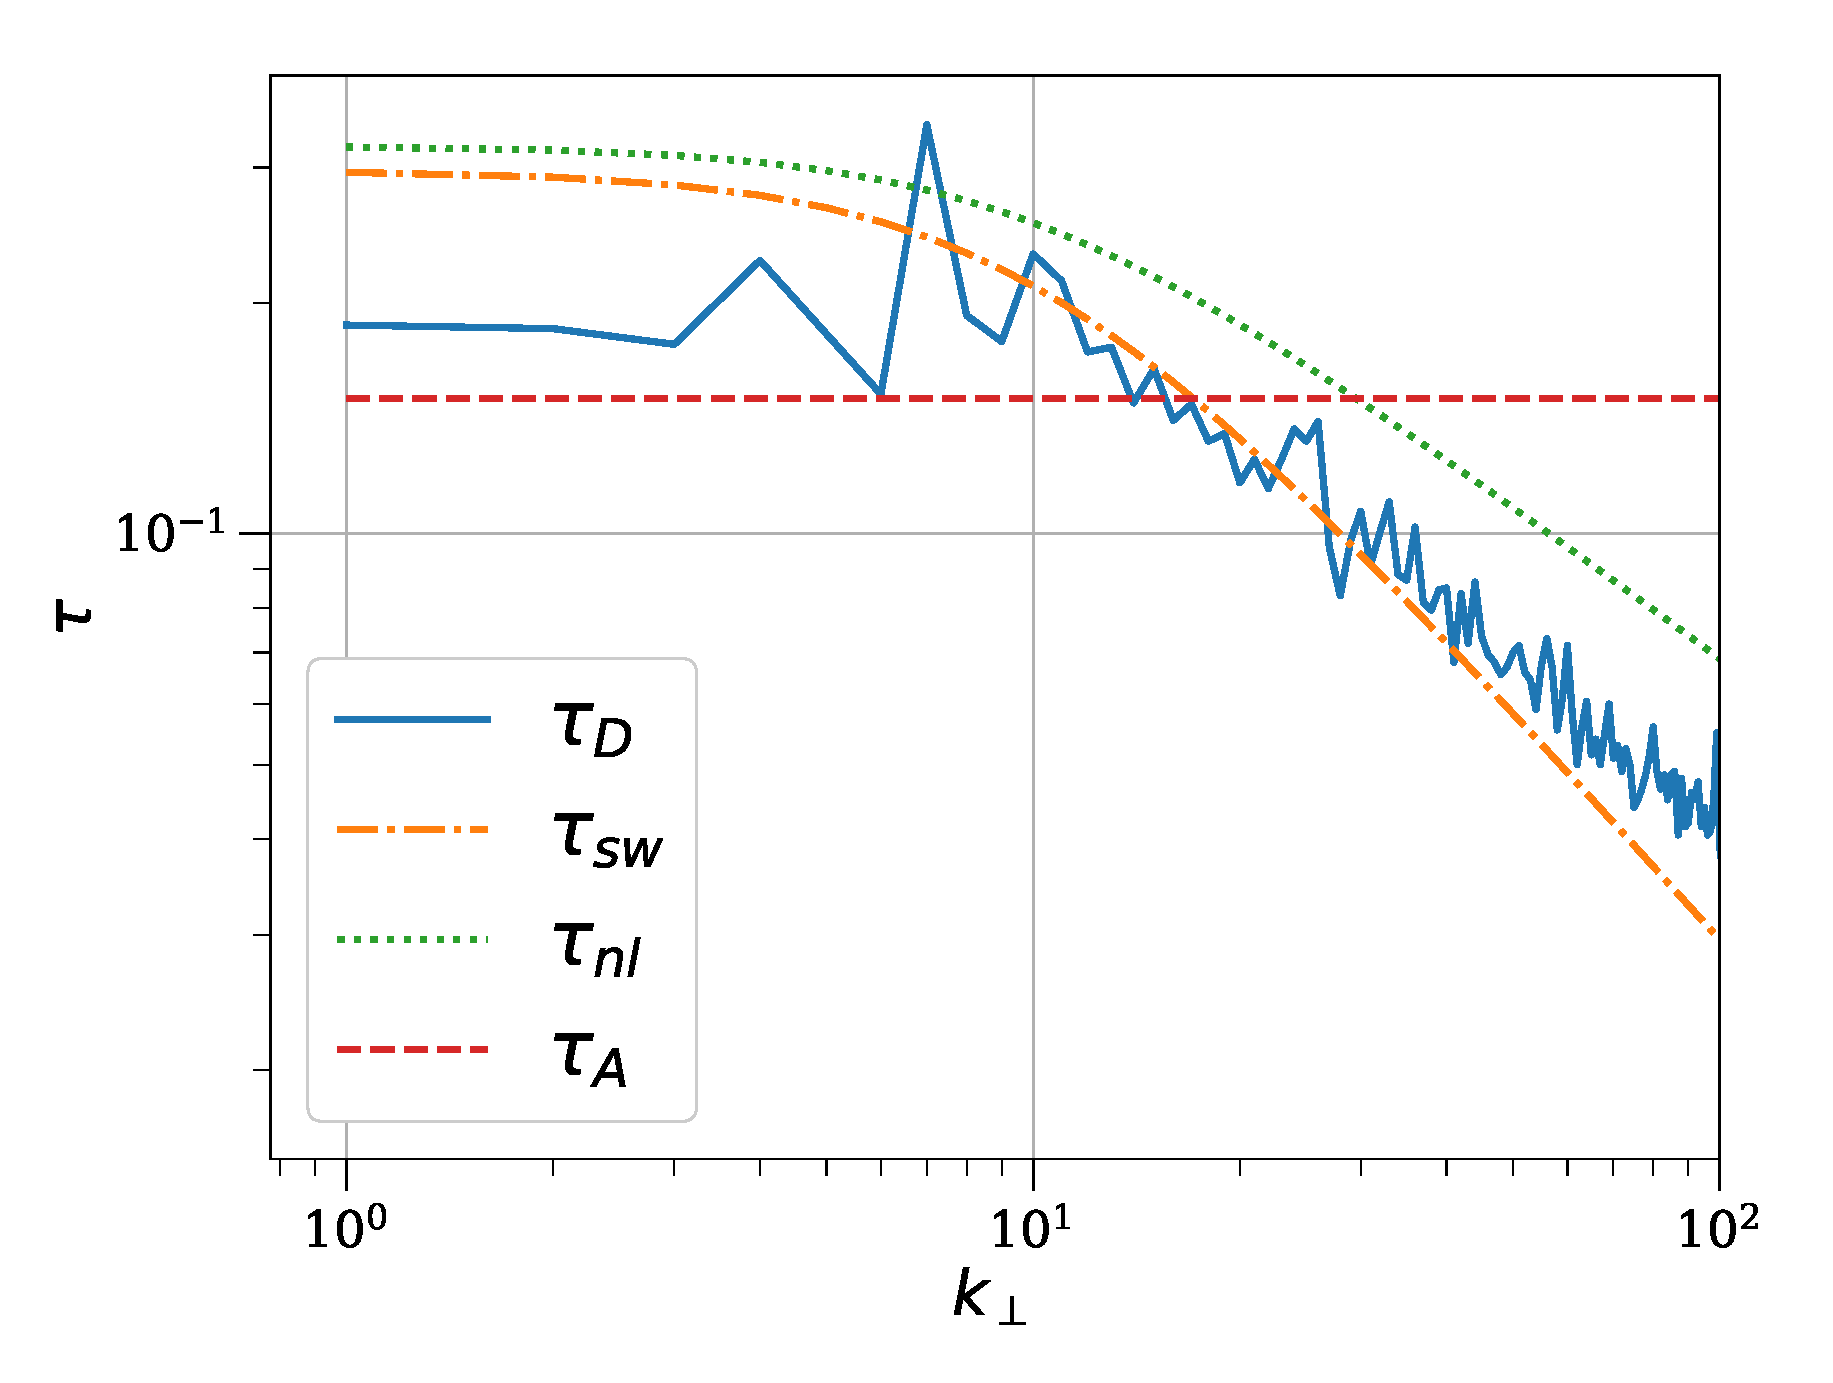
\includegraphics[width=1\textwidth]{P2/fig5_B1_Hc03_zmz_kpara_10.eps}
      \end{center}
    \end{minipage}
    \column{0.5\textwidth}
    \begin{minipage}[t]{1\textwidth}
      \begin{center}
        {$\vec{z}^+$} \\
        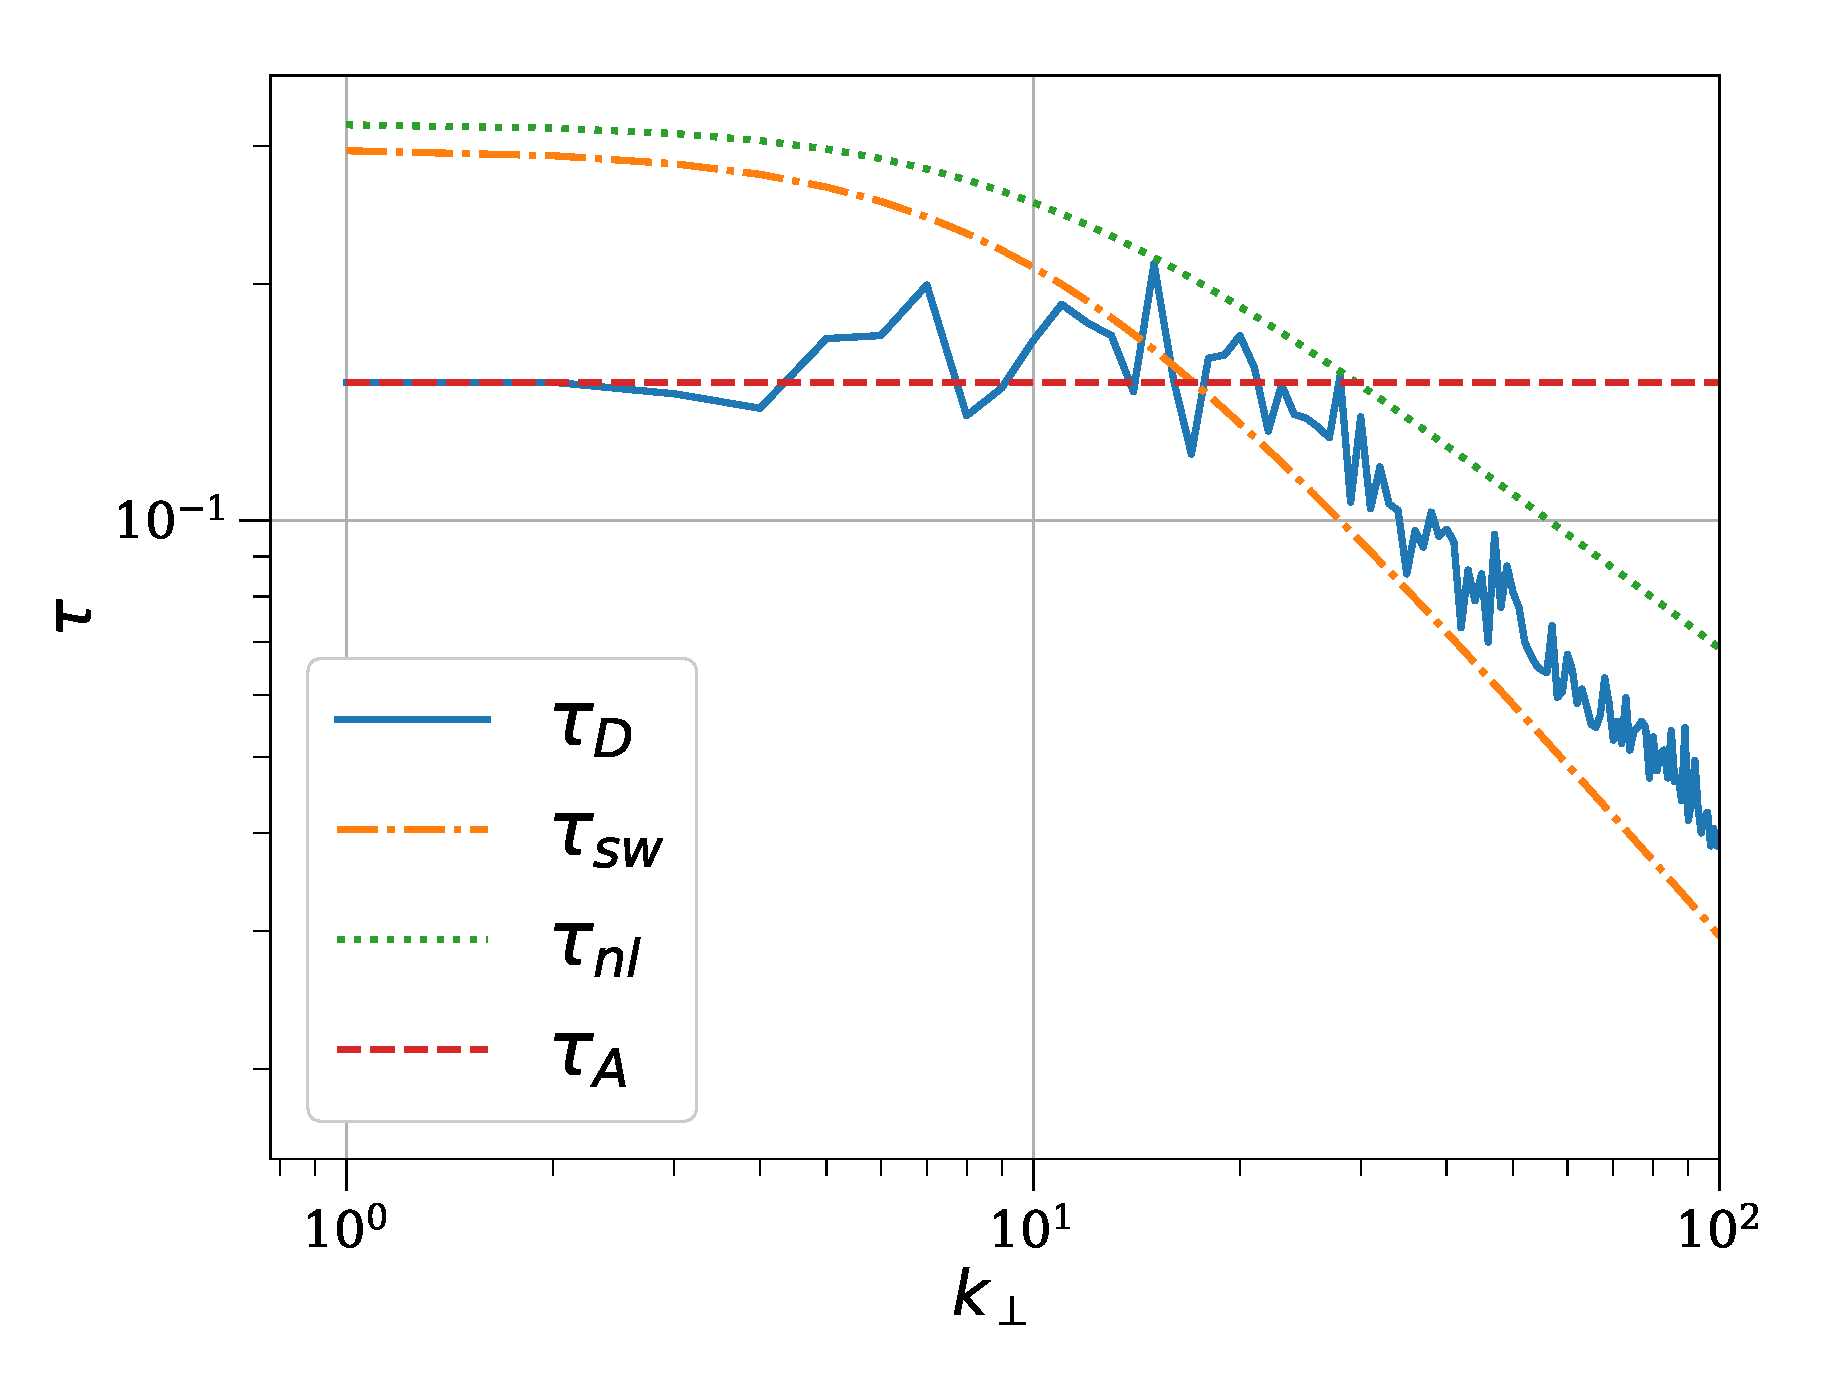
\includegraphics[width=1\textwidth]{P2/fig5_B1_Hc03_zpz_kpara_10.eps}
      \end{center}
    \end{minipage}
  \end{columns}
}
\note[itemize]{
\item No hay diferencias entre $\vec{z}^-$ y $\vec{z}^+$
\item Tiempo de Alfvén constante (no depende de $k_\perp$).
\item Alfvén para grandes escalas, \emph{sweeping} para pequeñas.
}






\frame{\frametitle{Tiempos de descorrelación}
  {\large \underline{Variación con $B_0$}} -  Casos con $\vec{z}^+$, $\sigma_c = 0.3$, $k_\parallel = 15$ \vspace{10pt}
  \begin{columns}
    \column{0.5\textwidth}
    \begin{minipage}[t]{1\textwidth}
      \begin{center}
        {$B_0 = 0.25$} \\
        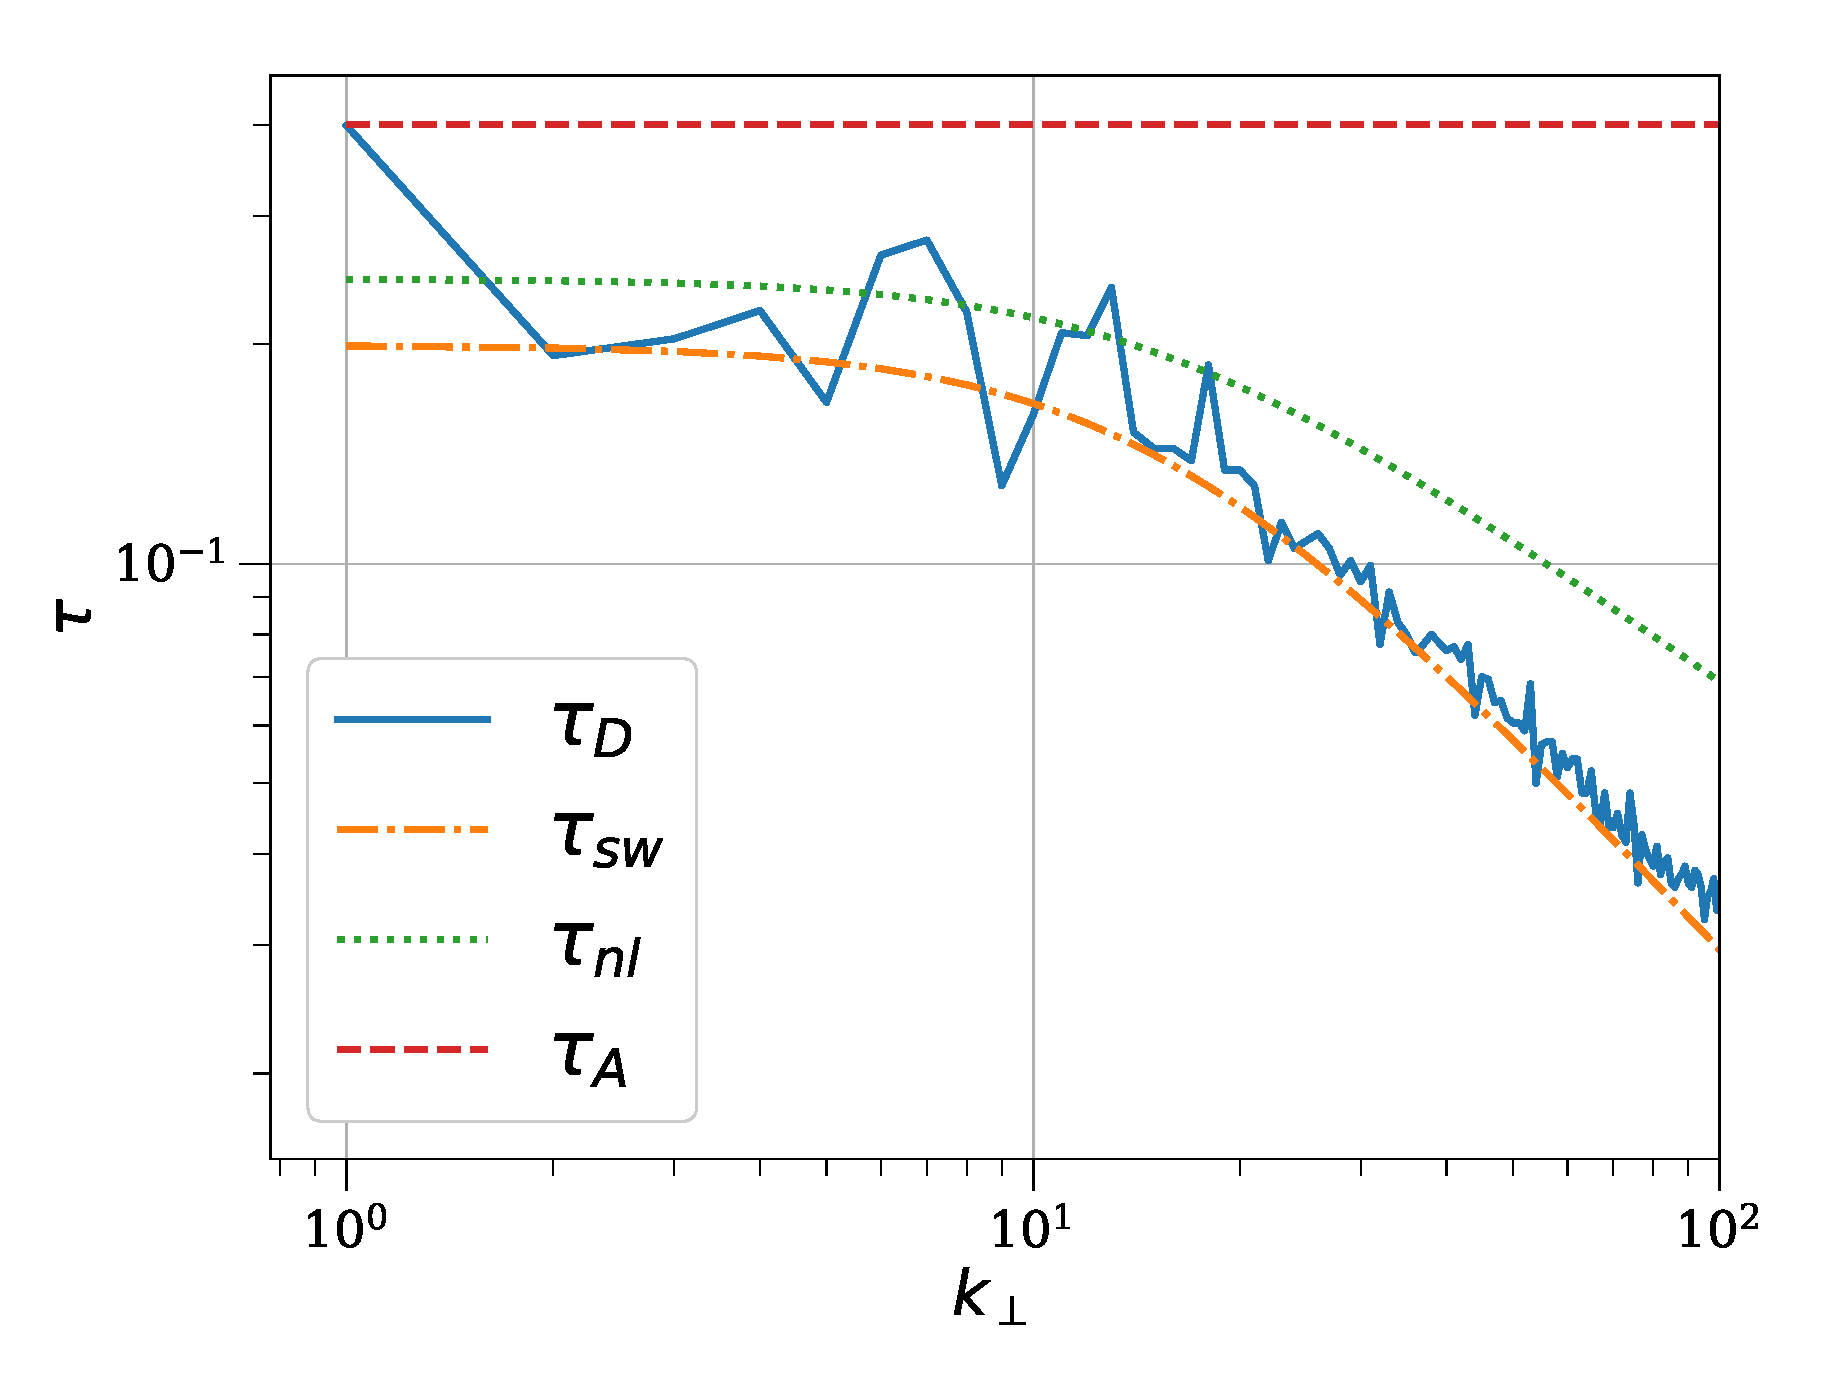
\includegraphics[width=0.65\textwidth]{P2/fig5_B025_Hc03_zpz_kpara_15.eps} \\
        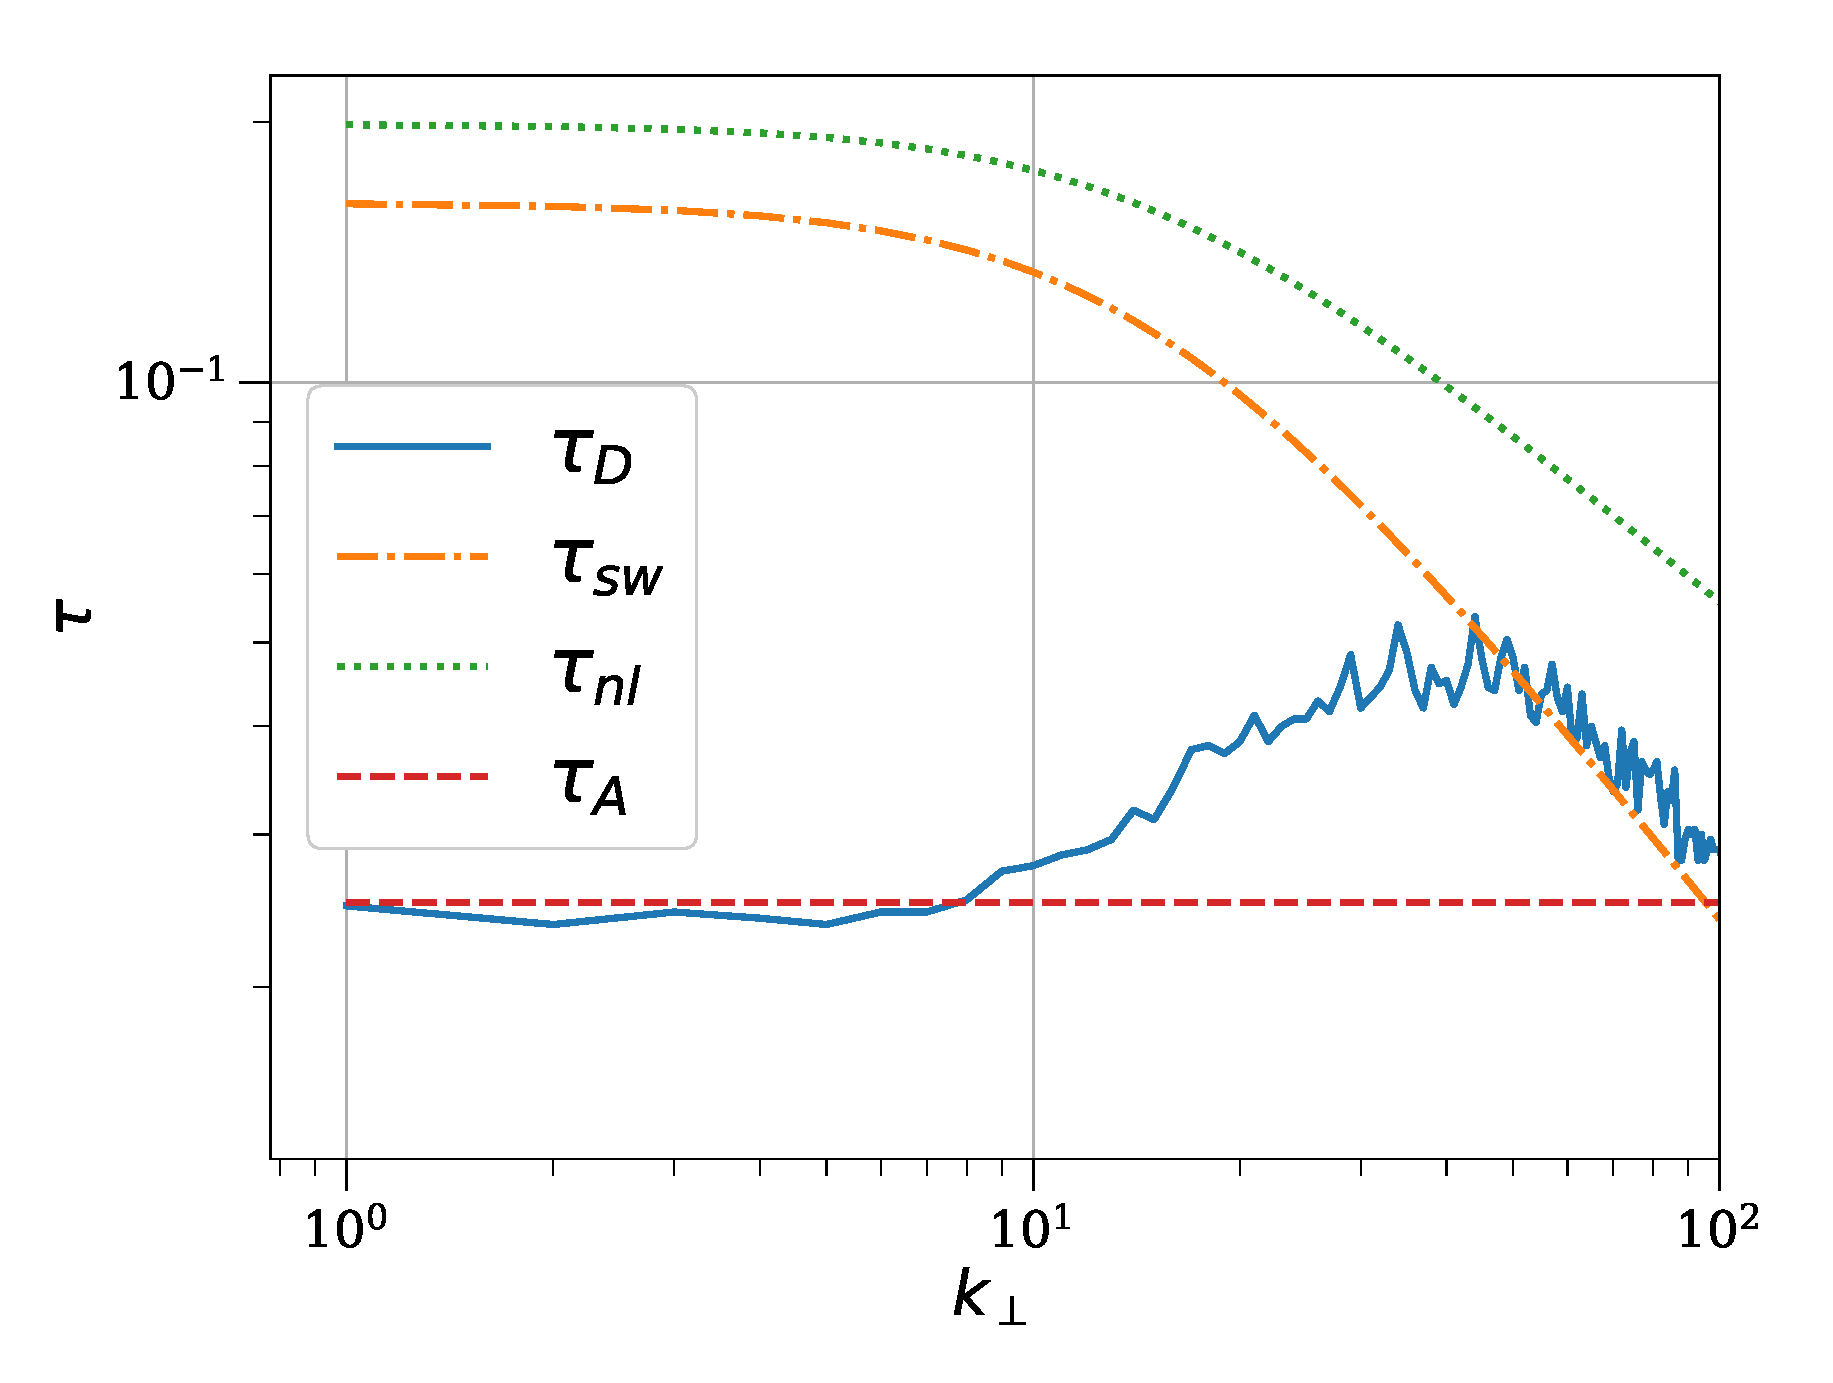
\includegraphics[width=0.65\textwidth]{P2/fig5_B4_Hc03_zpz_kpara_15.eps} \\
        {$B_0 = 4$}
      \end{center}
    \end{minipage}
    \column{0.5\textwidth}
    \begin{minipage}[t]{1\textwidth}
      \begin{center}
        {$B_0 = 1$} \\
        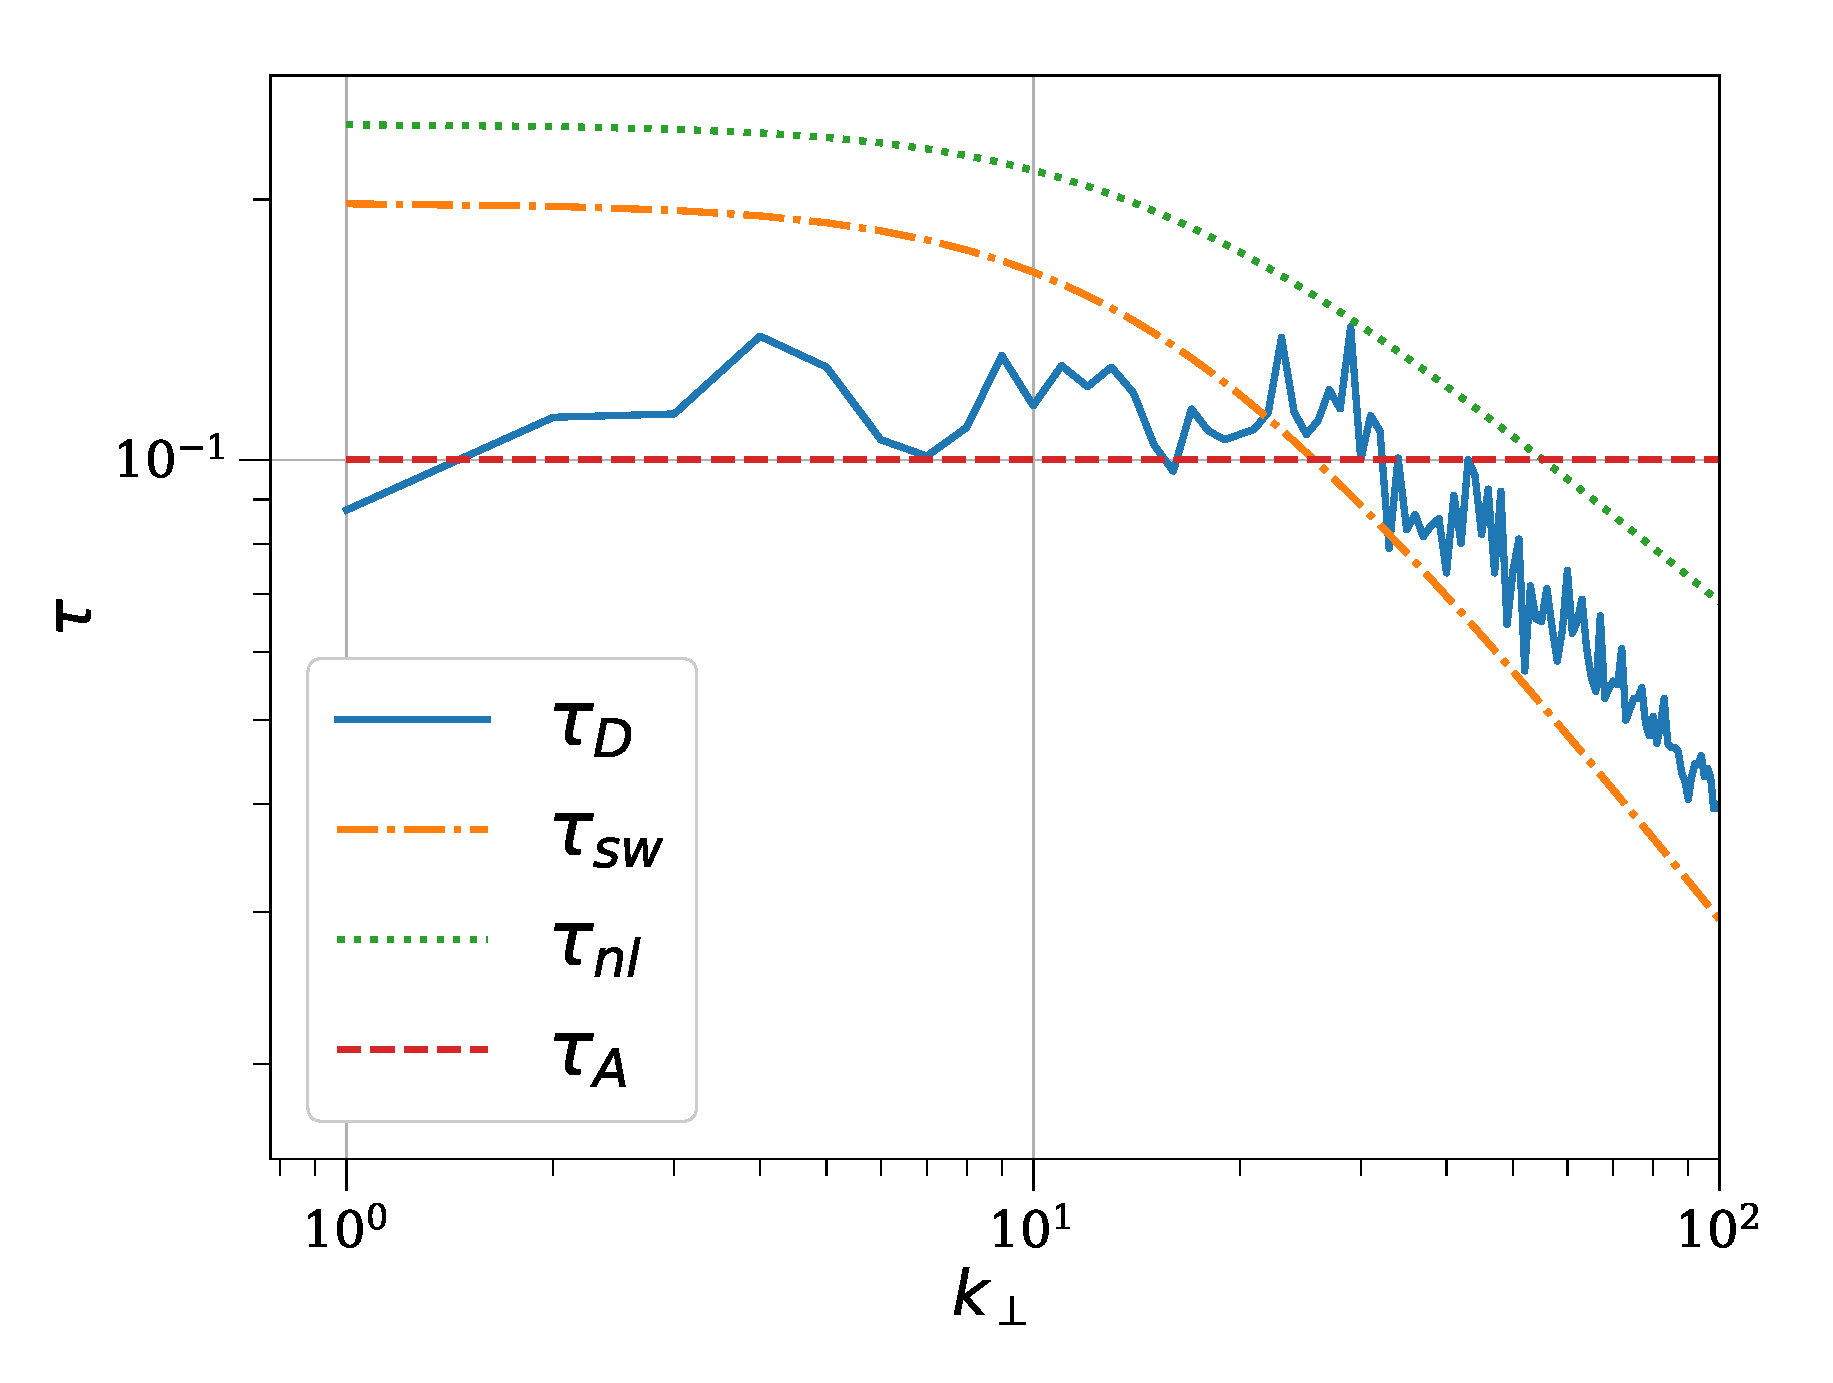
\includegraphics[width=0.65\textwidth]{P2/fig5_B1_Hc03_zpz_kpara_15.eps} \\
        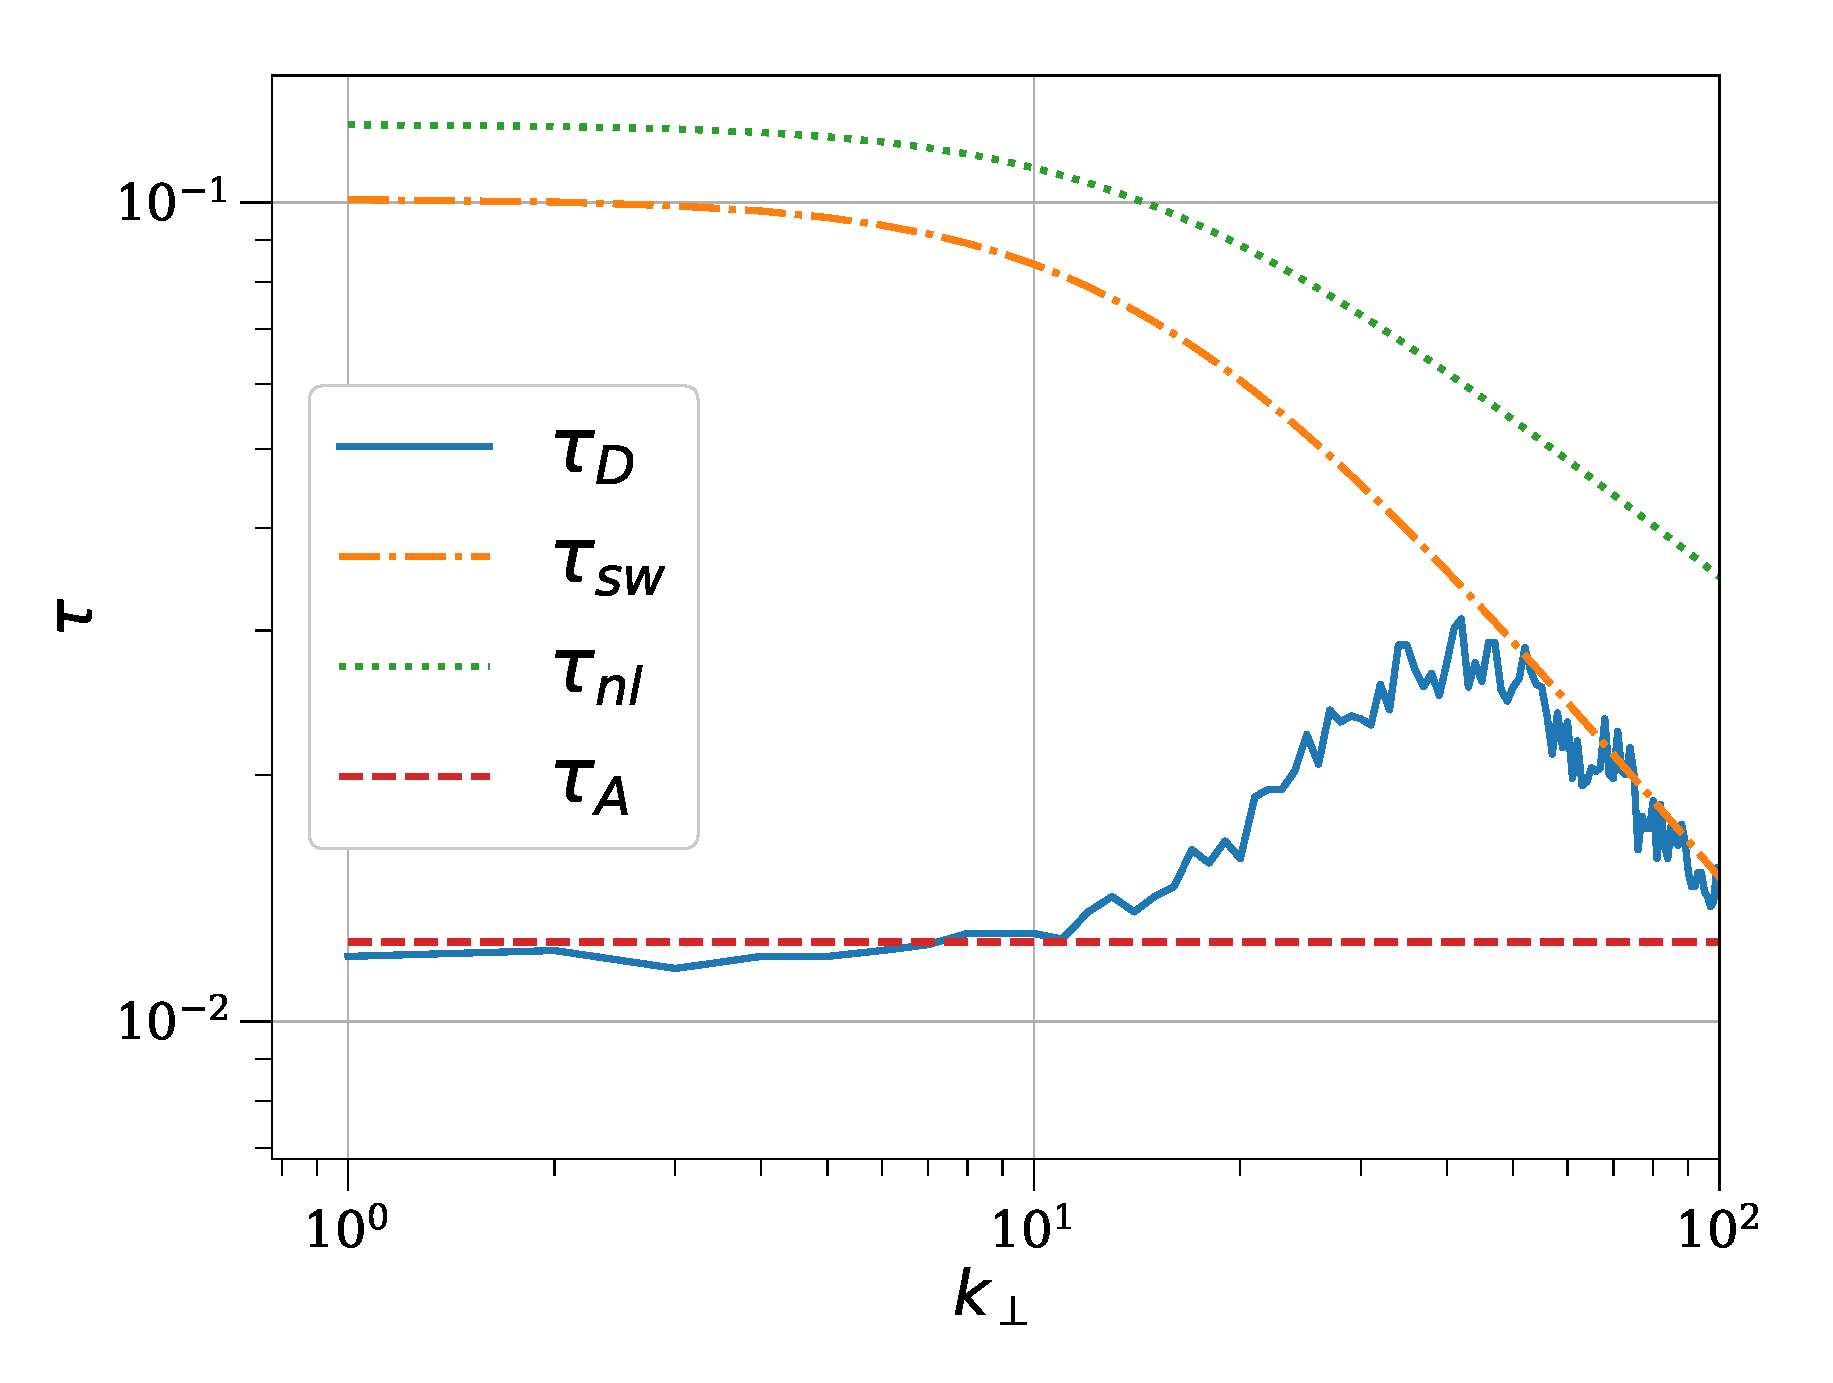
\includegraphics[width=0.65\textwidth]{P2/fig5_B8_Hc03_zpz_kpara_15.eps} \\
        {$B_0 = 8$}
      \end{center}
    \end{minipage}
  \end{columns}
}
\note[itemize]{
\item Valores bajos de $B_0$: $\tau_D$ dominado por el
  \emph{sweeping}.
\item Para valores más altos de $B_0$, los efectos Alfvénicos se
  vuelven dominantes.
\item En general, la escala temporal más rápida parece ser la
  dominante, resultado consistente con lo de P1.
\item Sin embargo, \textbf{la presencia de helicidad cruzada baja parece
  favorecer la transición hacia un flujo más dominado por las ondas de
  Alfvén}.
}



%% \frame{\frametitle{Tiempos de descorrelación}
%%   {\large \underline{Variación con $B_0$}} -  Casos con $\vec{z}^+$, $\sigma_c = 0.3$, $k_\perp = 15$ \vspace{10pt}
%%   \begin{columns}
%%     \column{0.5\textwidth}
%%     \begin{minipage}[t]{1\textwidth}
%%       \begin{center}
%%         {$B_0 = 0.25$} \\
%%         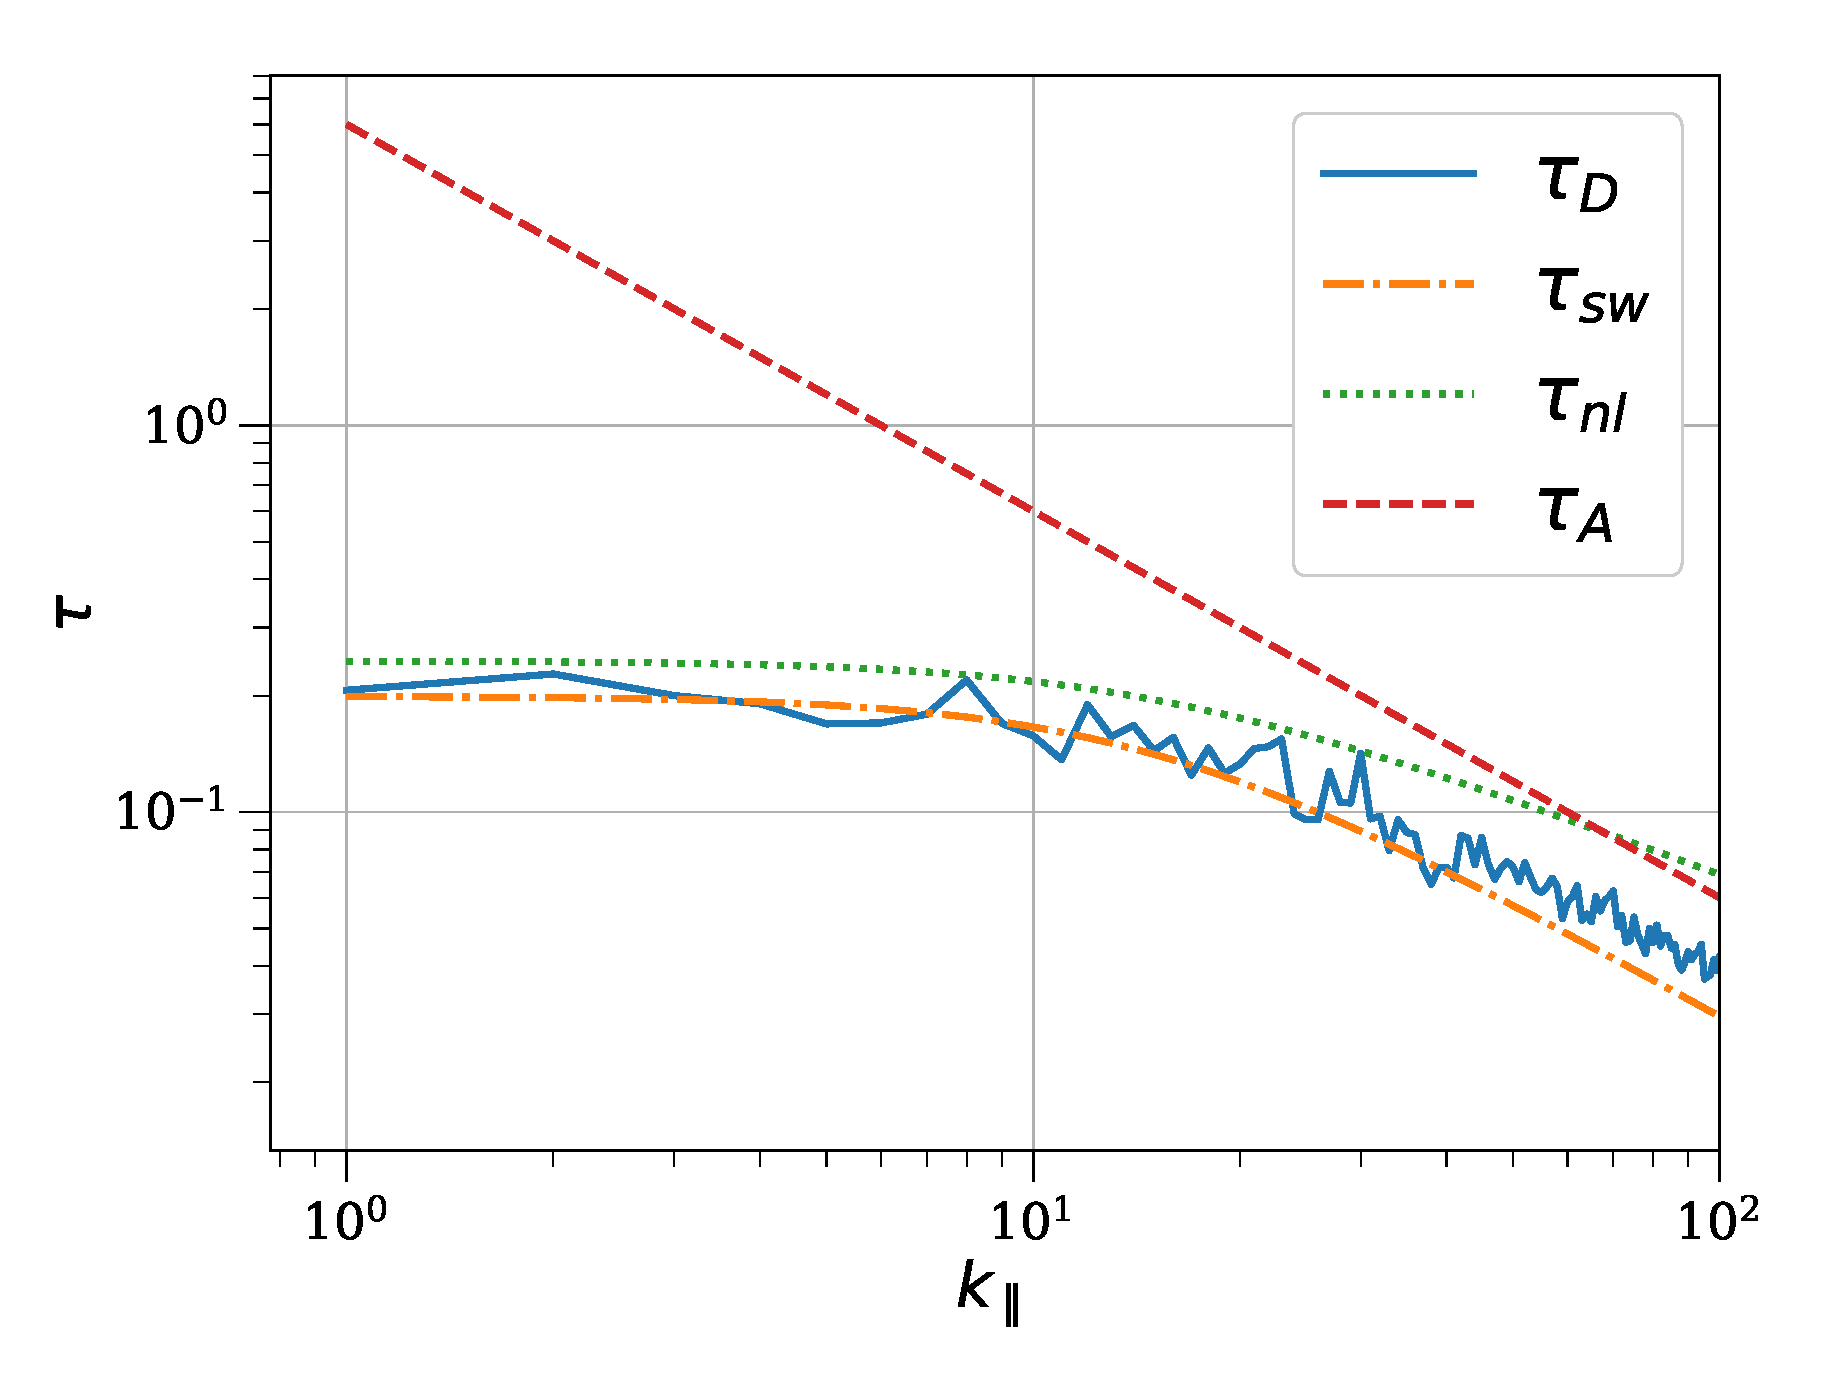
\includegraphics[width=0.65\textwidth]{P2/fig5_B025_Hc03_zpz_kperp_15.eps} \\
%%         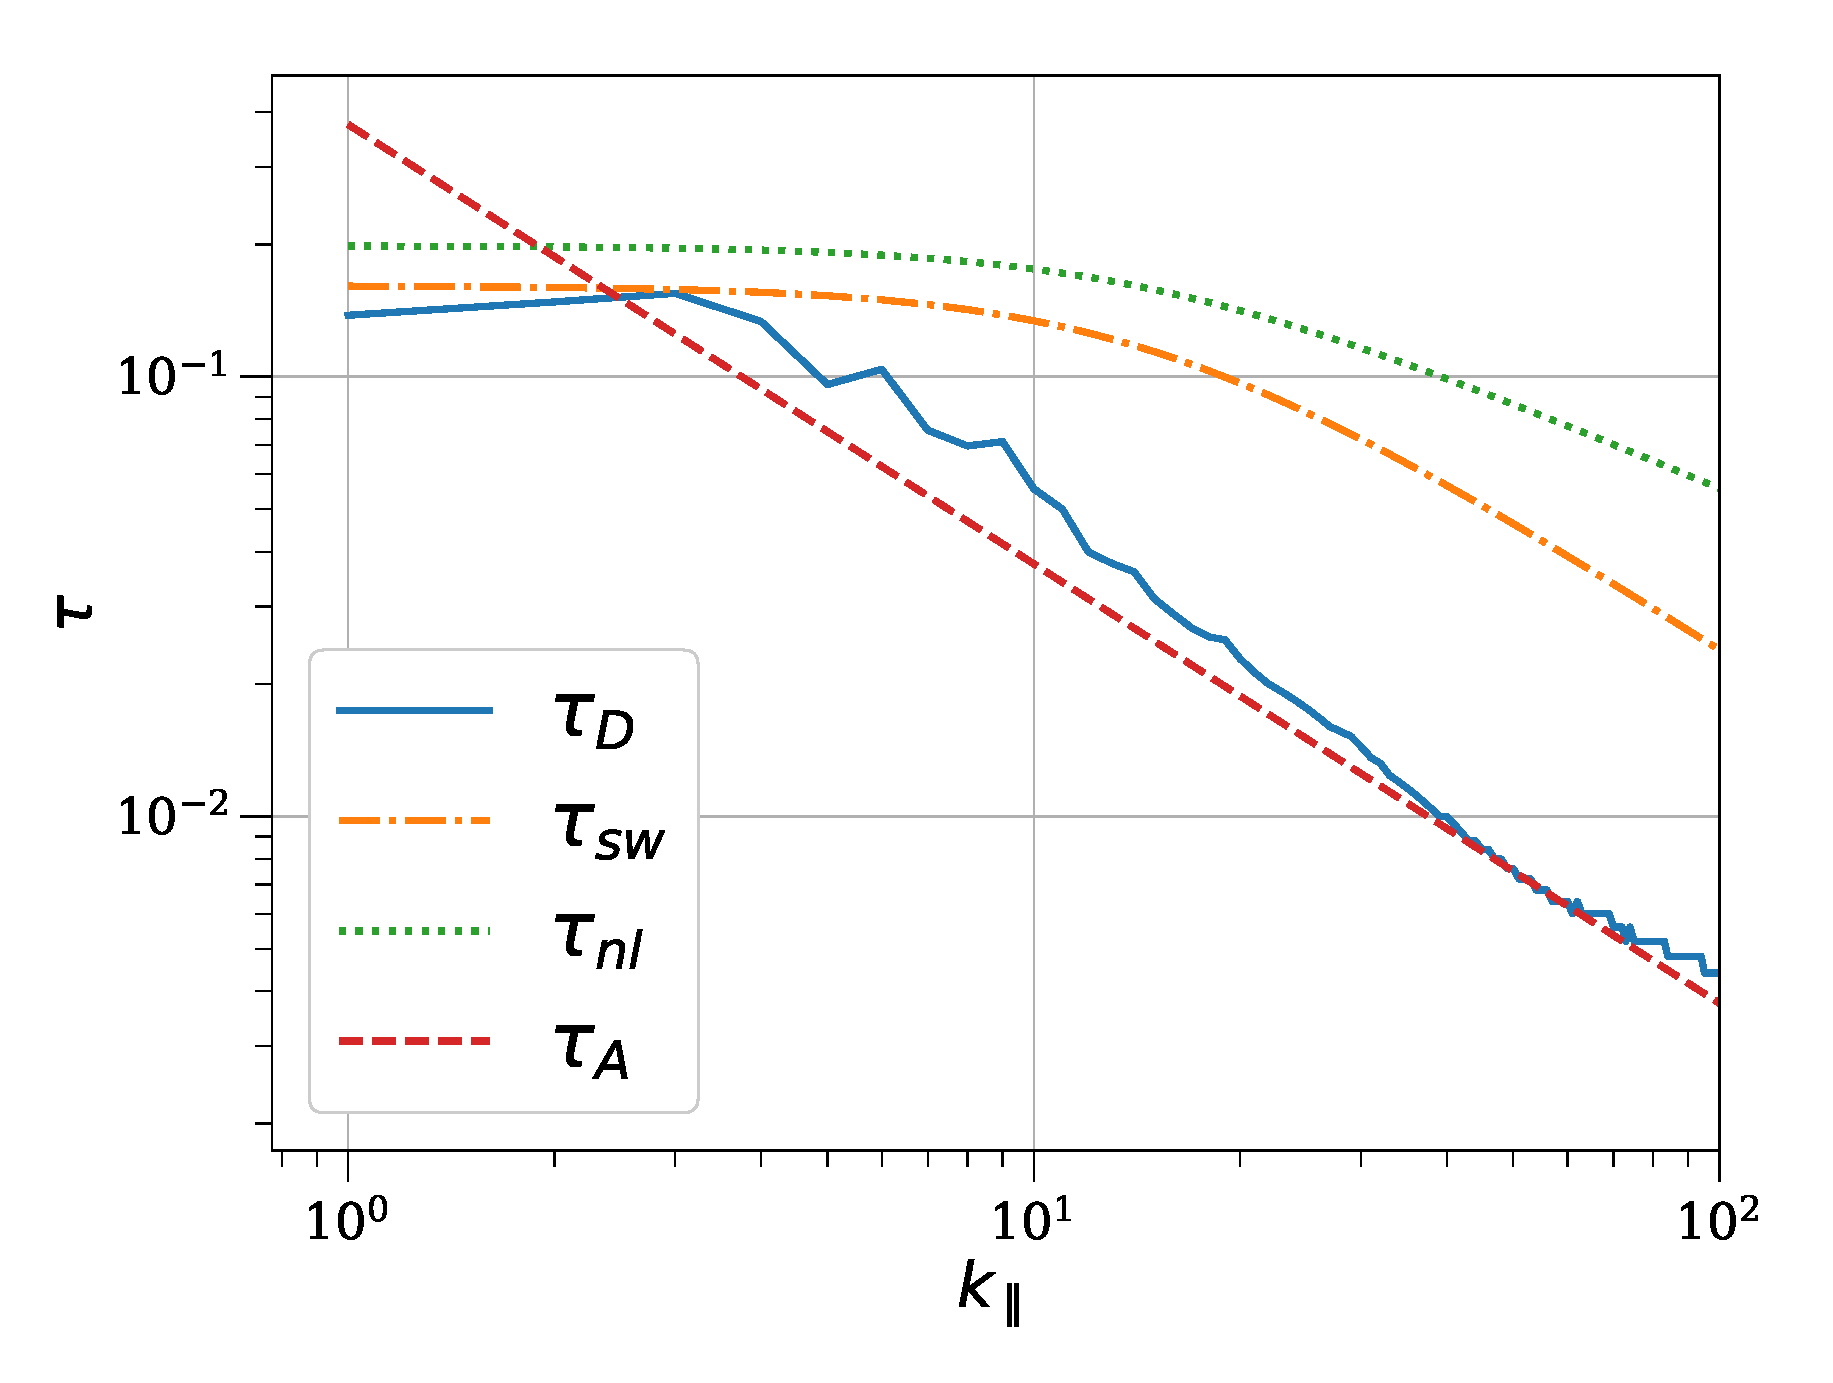
\includegraphics[width=0.65\textwidth]{P2/fig5_B4_Hc03_zpz_kperp_15.eps} \\
%%         {$B_0 = 4$}
%%       \end{center}
%%     \end{minipage}
%%     \column{0.5\textwidth}
%%     \begin{minipage}[t]{1\textwidth}
%%       \begin{center}
%%         {$B_0 = 1$} \\
%%         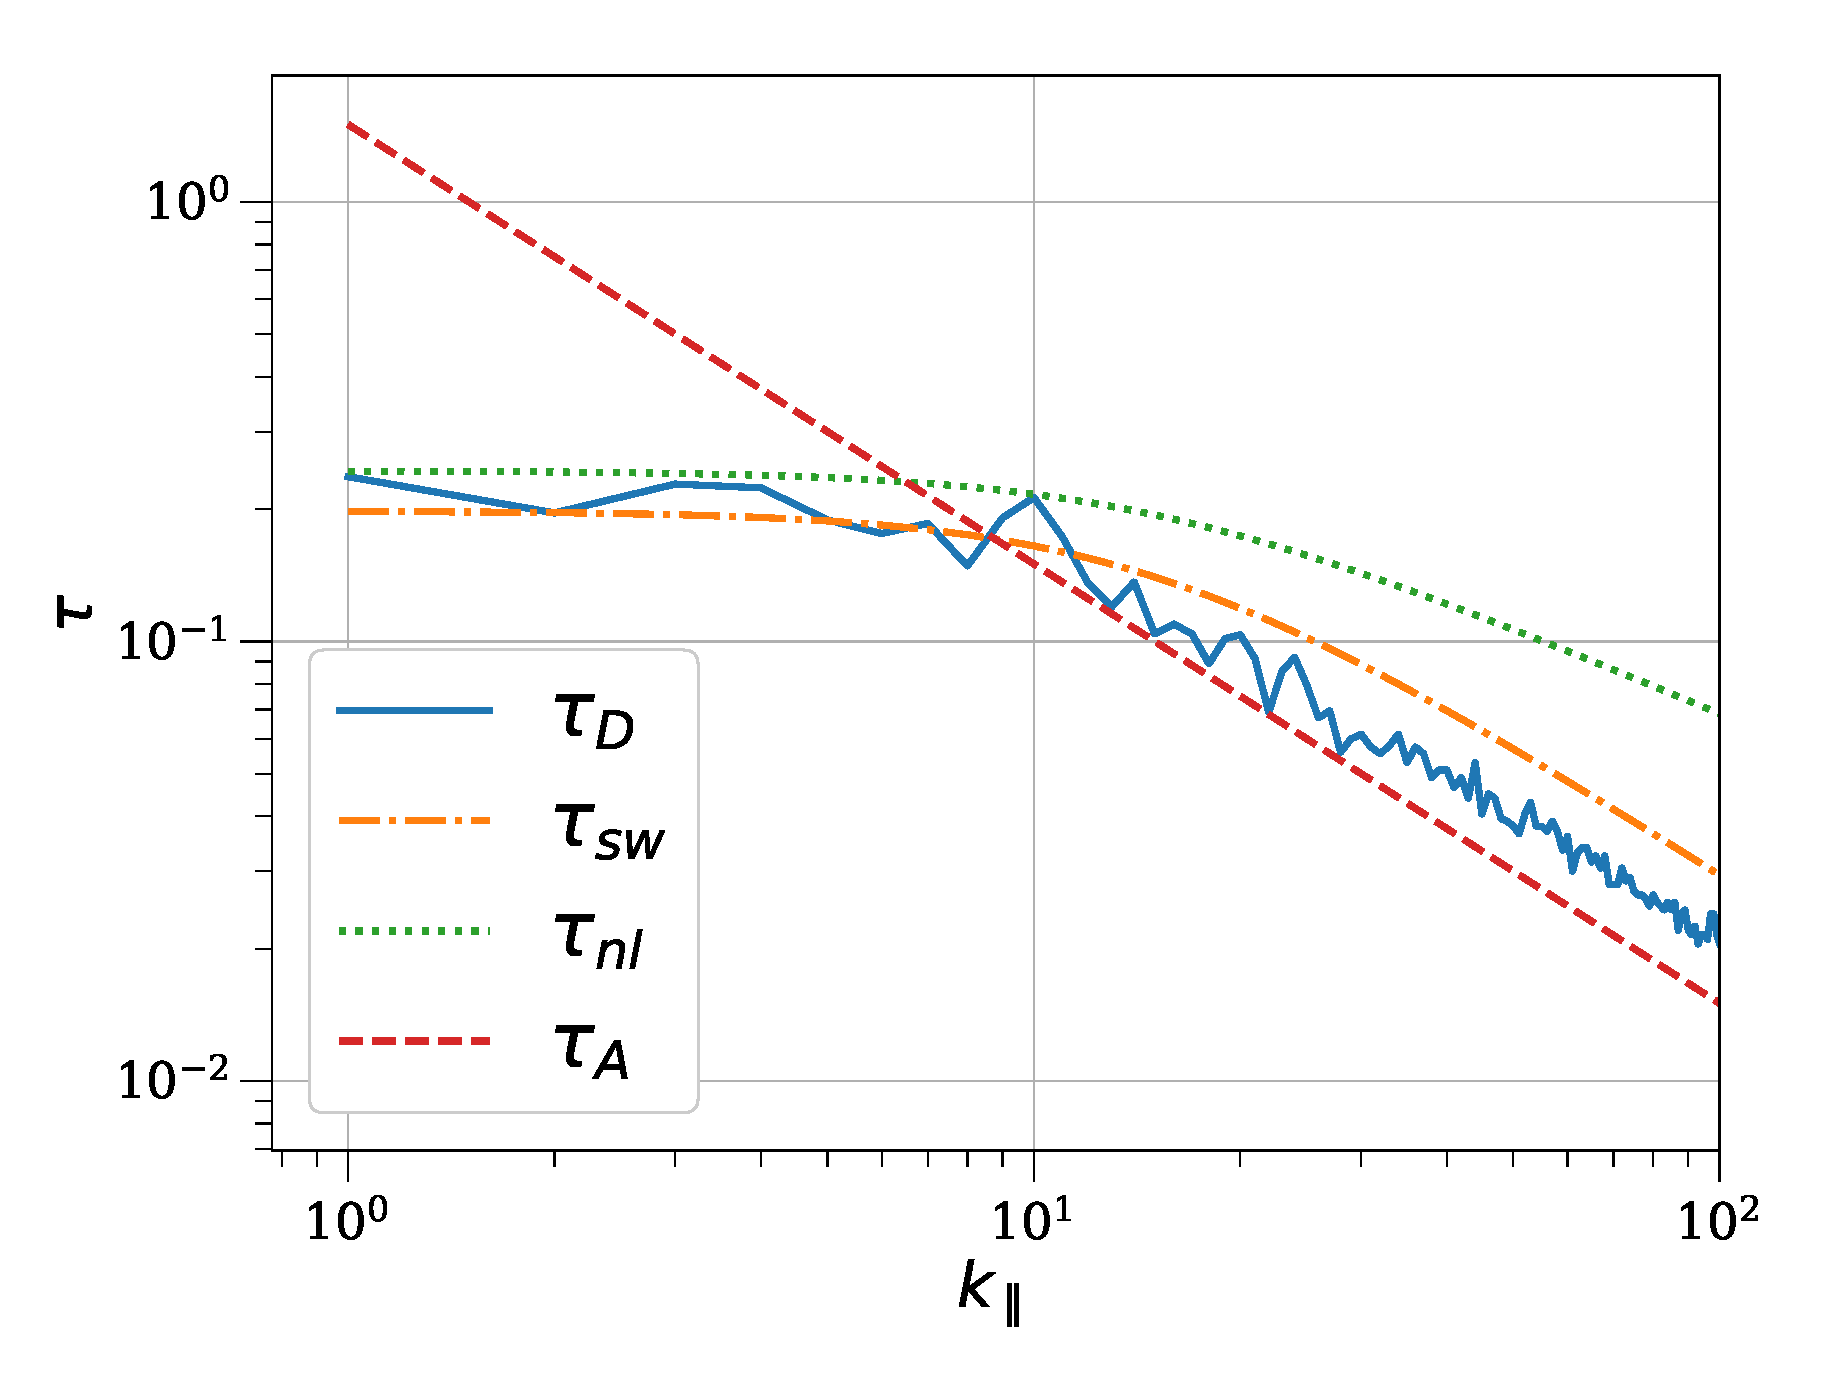
\includegraphics[width=0.65\textwidth]{P2/fig5_B1_Hc03_zpz_kperp_15.eps} \\
%%         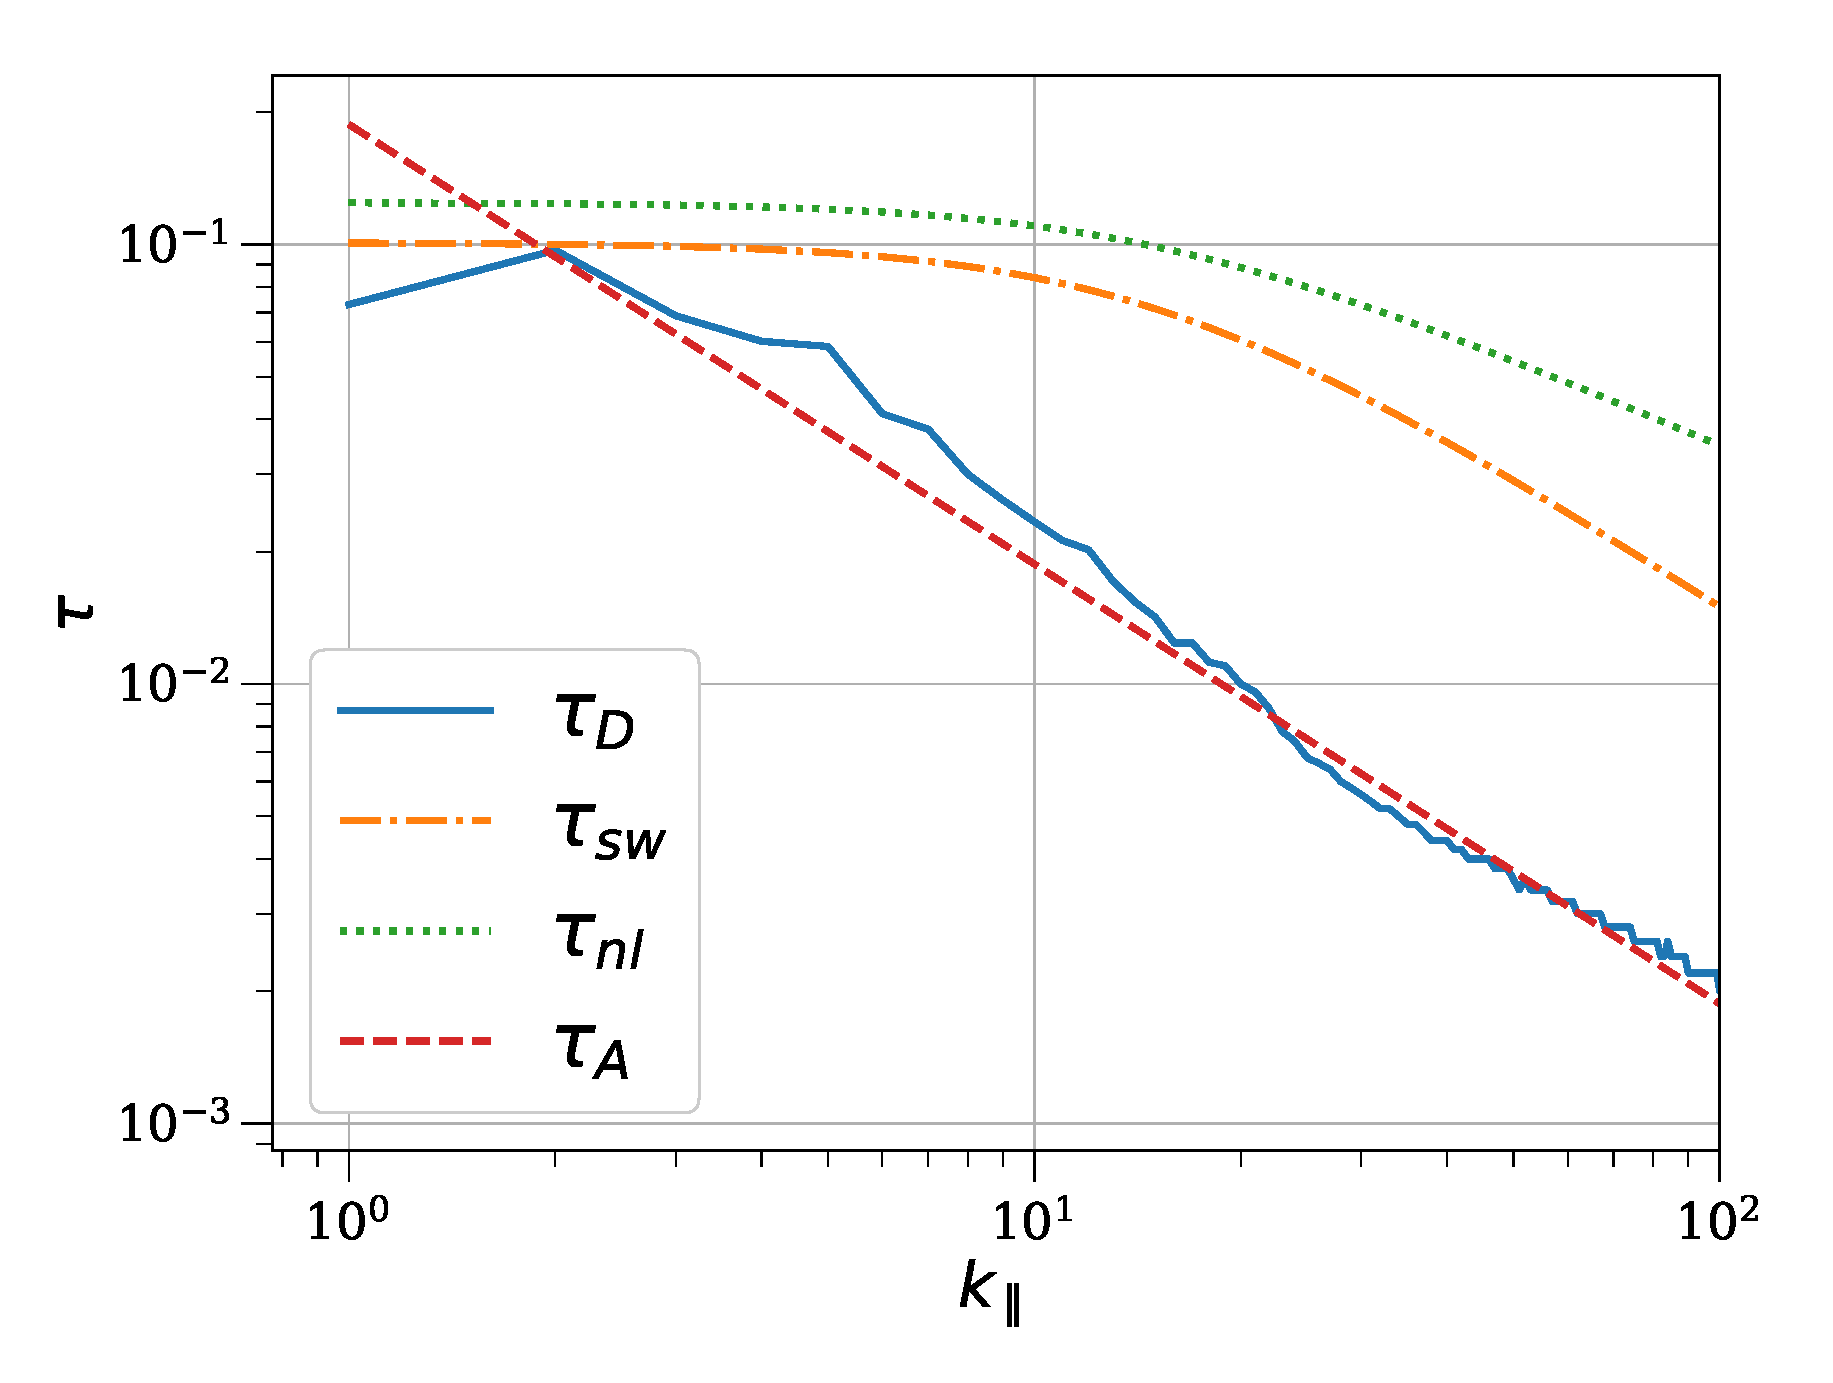
\includegraphics[width=0.65\textwidth]{P2/fig5_B8_Hc03_zpz_kperp_15.eps} \\
%%         {$B_0 = 8$}
%%       \end{center}
%%     \end{minipage}
%%   \end{columns}
%% }
%% \note[itemize]{
%% \item El resultado es similar al anterior.
%% }



\frame{\frametitle{Tiempos de descorrelación}
  {\large \underline{Variación con $\sigma_c$}} -  Casos con $\vec{z}^+$, $B_0 = 1$, $k_\perp = 40$
  \begin{columns}
    \column{0.5\textwidth}
    \begin{minipage}[t]{1\textwidth}
      \begin{center}
        $\sigma_c = 0.0$\\
        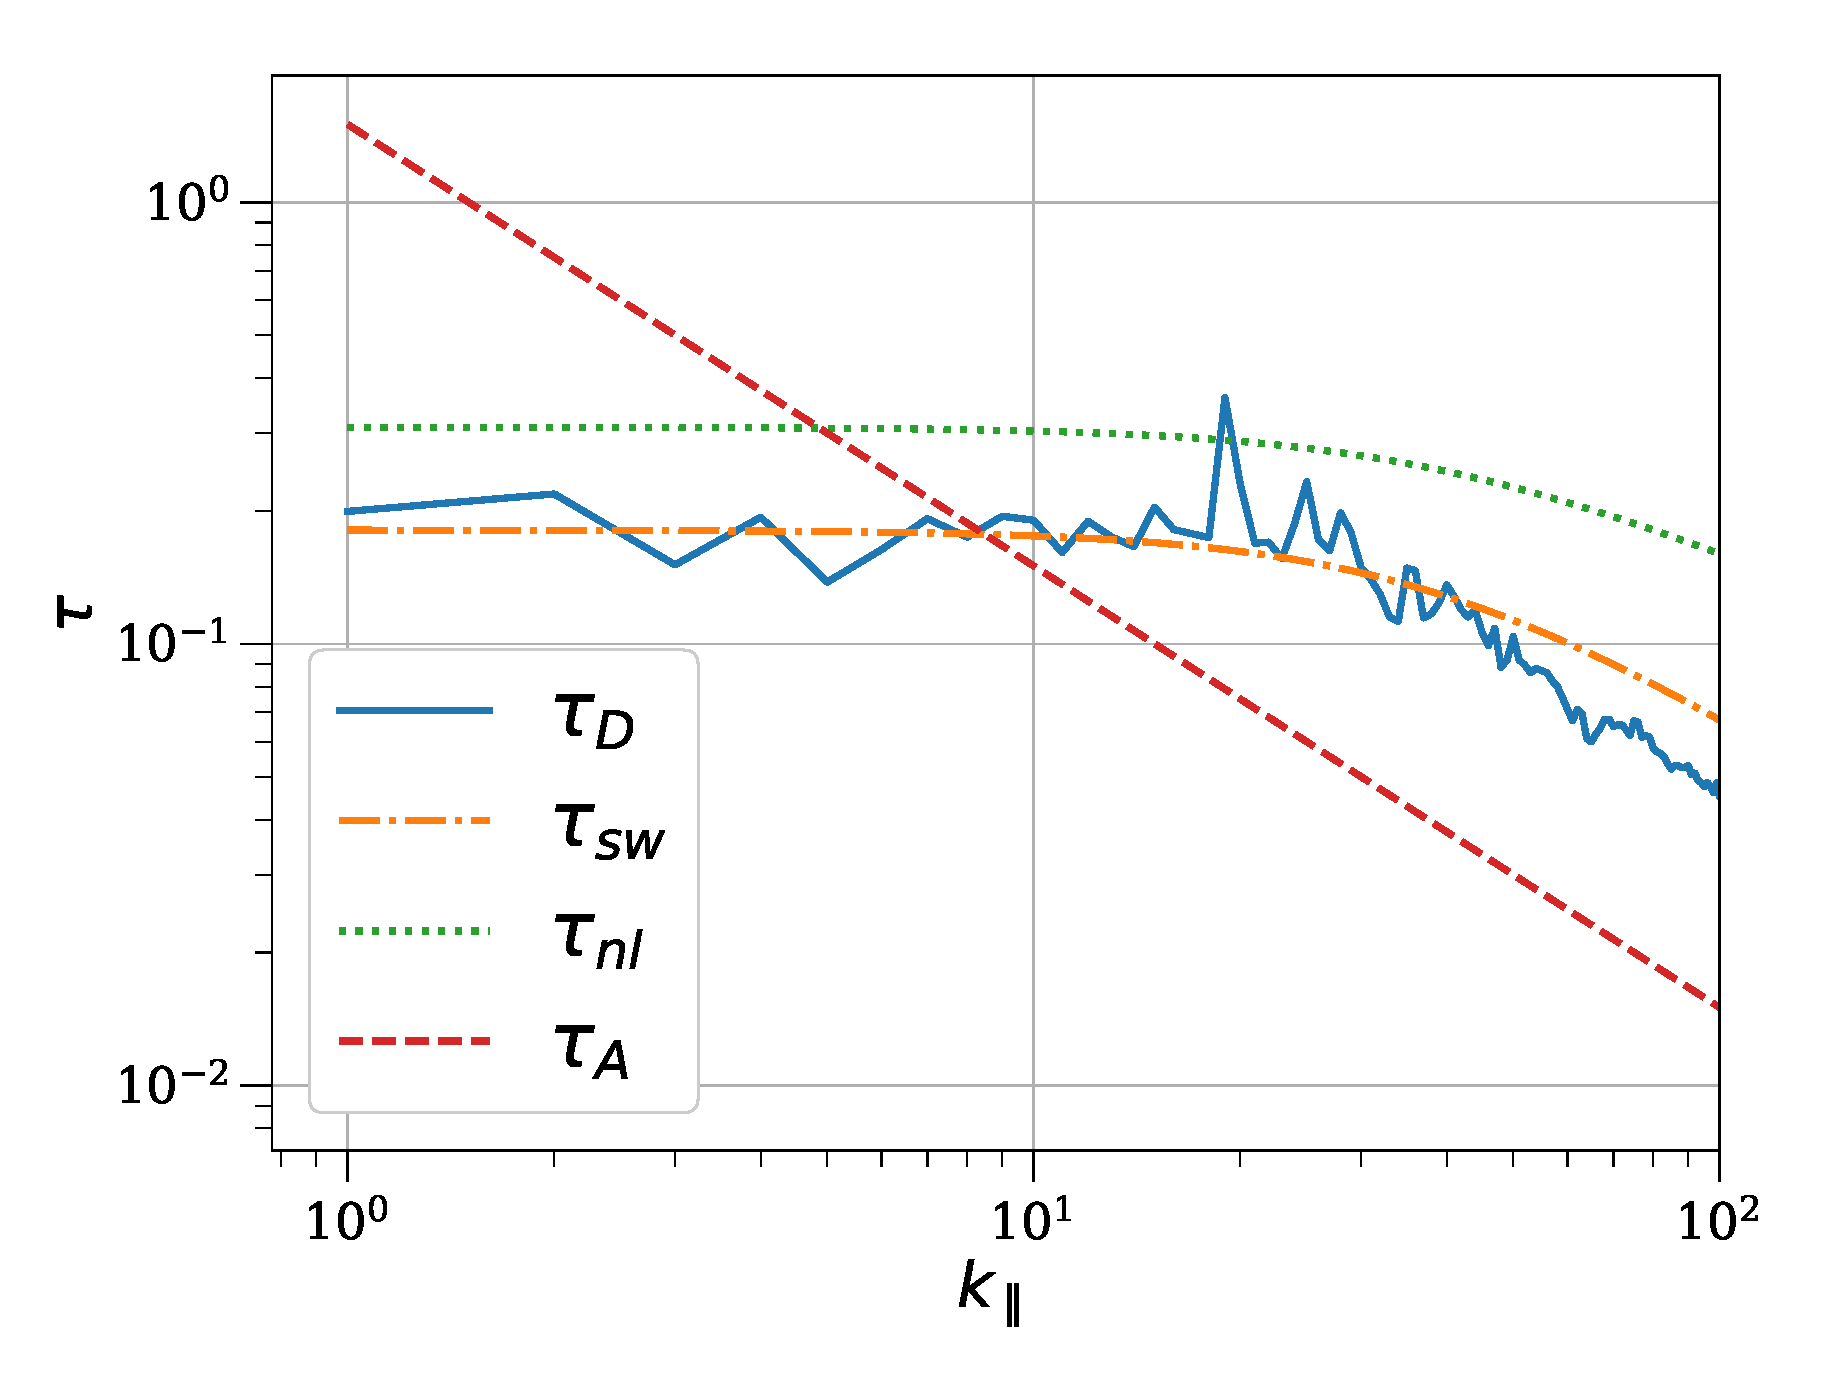
\includegraphics[width=0.76\textwidth]{P2/fig5_B1_Hc00_zpz_kperp_40.eps}
      \end{center}
    \end{minipage}
    \column{0.5\textwidth}
    \begin{minipage}[t]{1\textwidth}
      \begin{center}
        $\sigma_c = 0.3$\\
        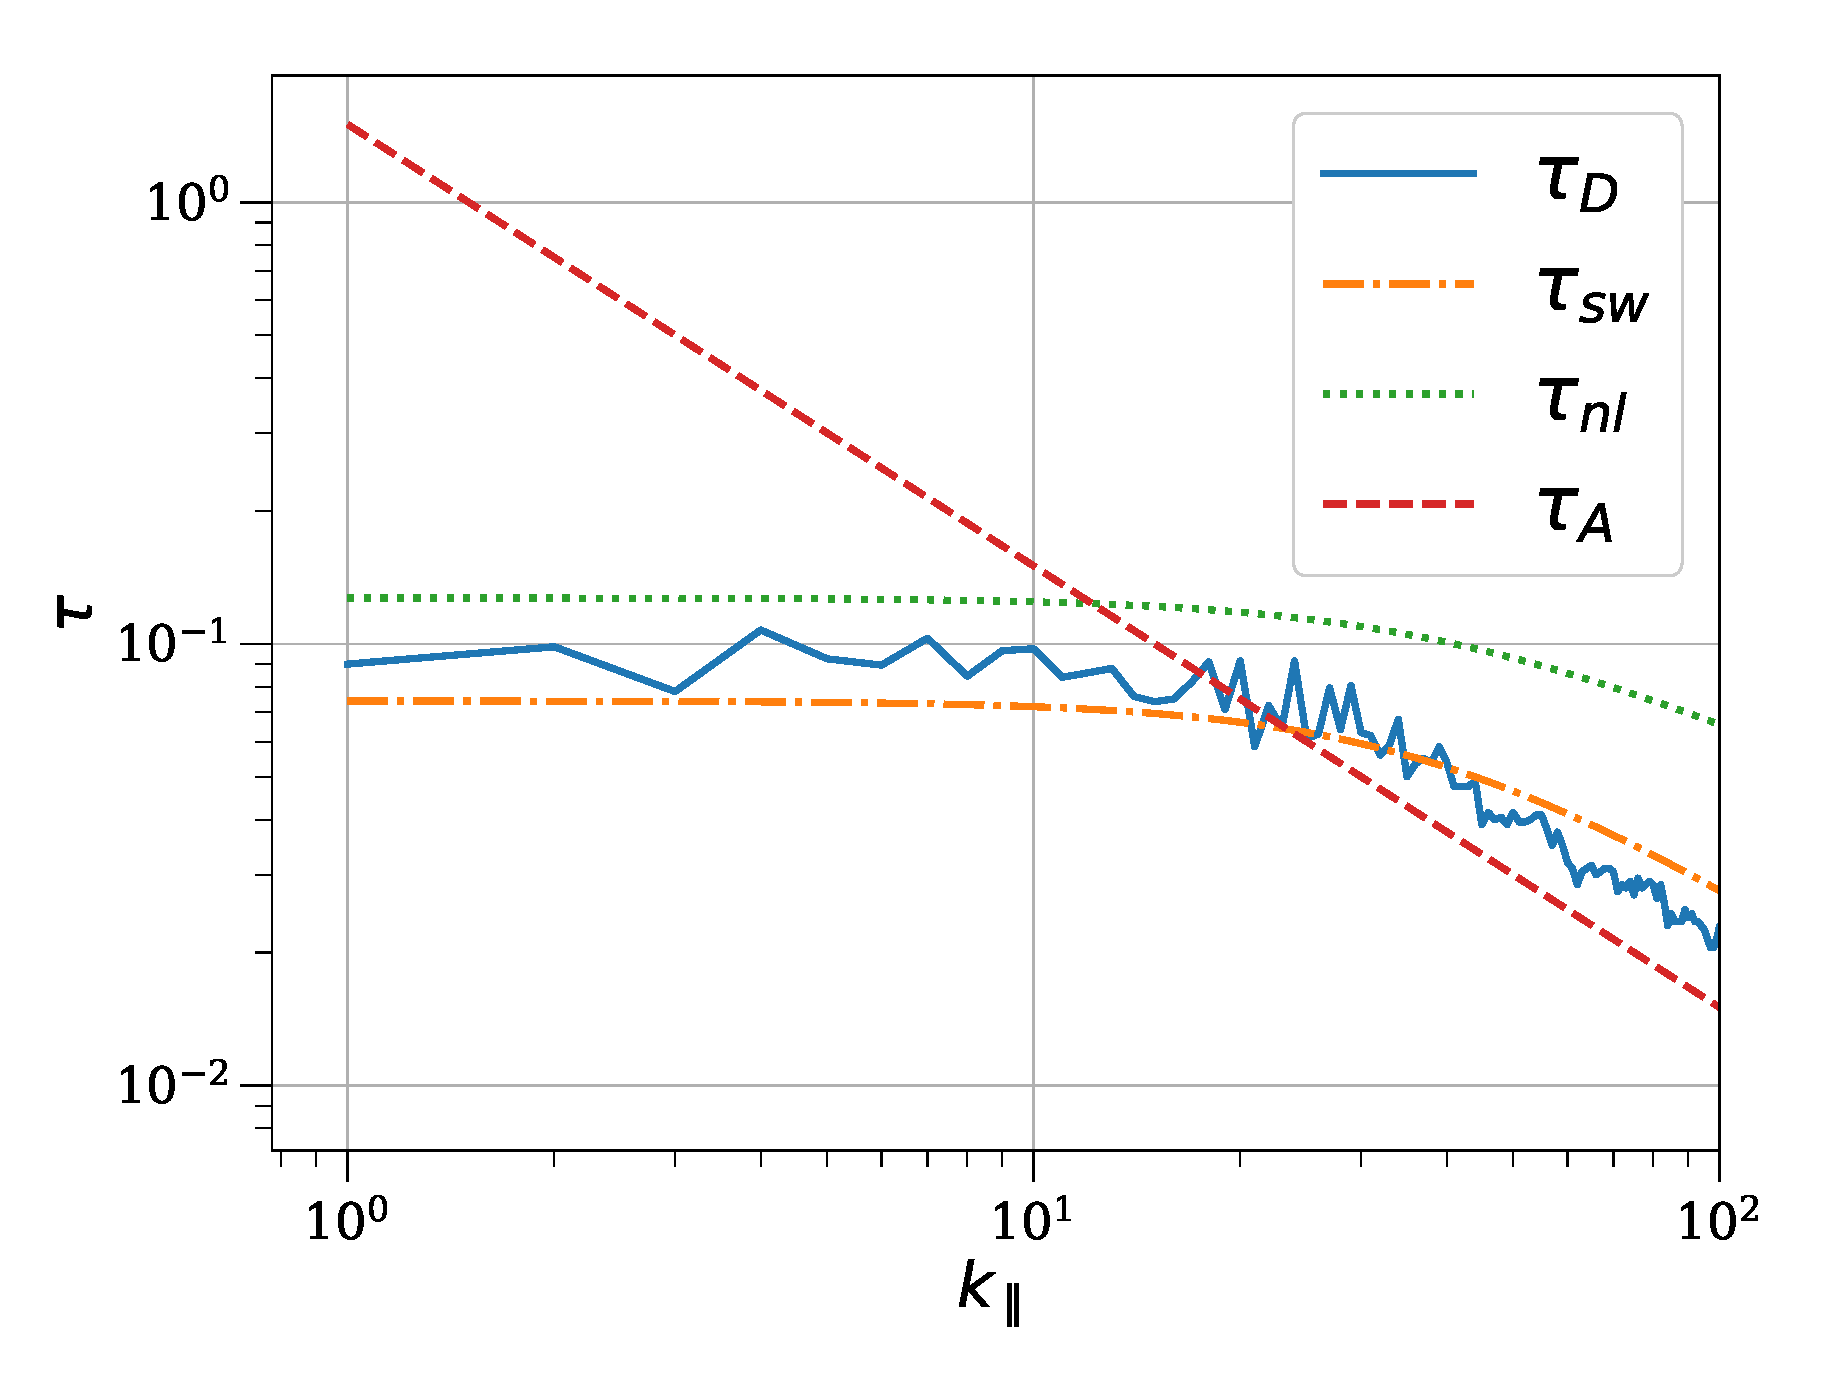
\includegraphics[width=0.76\textwidth]{P2/fig5_B1_Hc03_zpz_kperp_40.eps}
      \end{center}
    \end{minipage}
  \end{columns}
  \vspace{-0.5cm}
  \begin{center}
    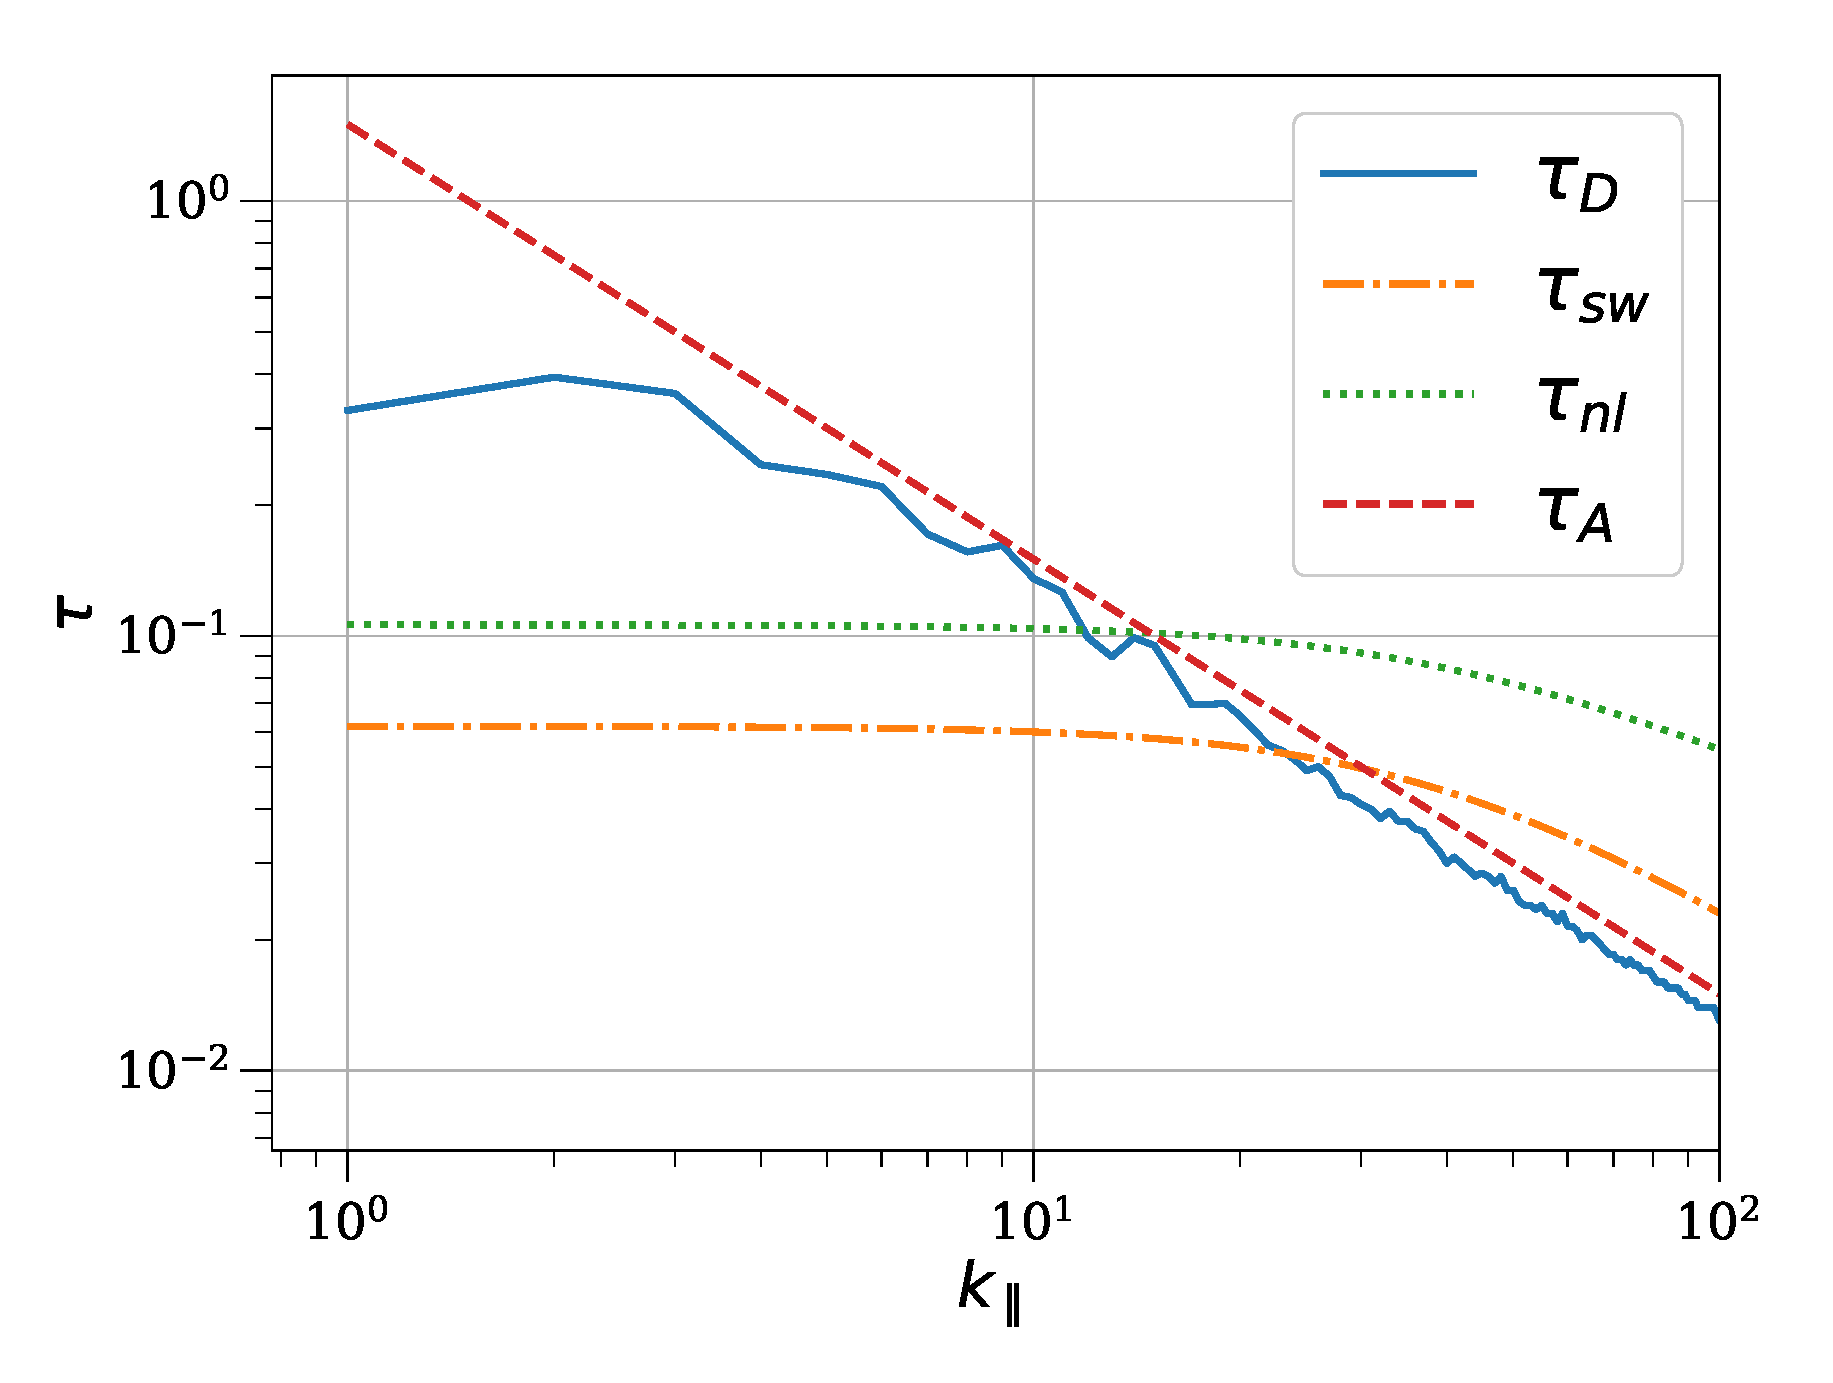
\includegraphics[width=0.38\textwidth]{P2/fig5_B1_Hc09_zpz_kperp_40.eps}\\
    $\sigma_c = 0.9$
  \end{center}
}
\note[itemize]{
\item Para valores bajos de $\sigma_c$, se confirman los resultados del P1.
\item Sin embargo, incrementar la helicidad cruzada del flujo tiene
  consecuencias muy interesantes.
\item \textbf{Alto $\sigma_c$, Alfvén domina, aun cuando sea más lento que las otras escalas
  temporales.}
\item \textbf{Esto es consistente con la imagen en la que la mayoría
  de las fluctuaciones tienen una única dirección de propagación (sólo
  $\vec{z}^+$)}.
}



\frame{\frametitle{Conclusiones}
\pause
  \begin{itemize}
  \item Los tiempos de descorrelación son dominados por los efectos de
    \textit{sweeping} para valores bajos del campo magnético medio y
    de la helicidad cruzada, y \textbf{por los efectos Alfvénicos para valores
    grandes} del campo magnético medio o \textbf{de helicidad cruzada, aún
    cuando $\tau_A$ no sea el más rápido}.
  \item En principio, este comportamiento puede ser interpretado como
    una transición hacia un régimen con no-linealidades más débiles a
    medida que se incrementa la helicidad cruzada, como suele ser
    discutido teóricamente y como aparentemente indican nuestras
    simulaciones numéricas.
  \end{itemize}
}
\note[itemize]{
\item 1) una nueva característica cuando lo comparamos con estudios
previos del comportamiento espacio-temporal de turbulencia MHD fuerte
con helicidad cruzada nula
}


\frame{\frametitle{Conclusiones}
  \begin{itemize}
  \item Encontramos un régimen en el que se generan fluctuaciones
    $\vec{z}^-$ y $\vec{z}^+$ (polarizaciones opuestas), y se propagan
    en la misma dirección debido a la reflexión de ondas, causada por
    inhomogeneidades del campo magnético de gran escala.
  \item Así, el análisis espacio-temporal de los flujos turbulentos
    provee evidencia directa de un fenómeno predicho anteriormente con
    la teoría WKB, y puede jugar un rol relevante modificando la
    propagación de ondas y las interacciones no lineales en el medio
    interplanetario.
  \end{itemize}
}
\note[itemize]{
\item 1) Cuando la componente uniforme y constante del campo magnético
  de gran escala no es demasiado fuerte.
}


\frame{\frametitle{Conclusiones}
  \begin{itemize}
  \item Los resultados muestran que, al menos en turbulencia fuerte, la
    representación de ondas no es suficientemente completa para
    describir el sistema de MHD incompresible.
  \item Fenómenos físicamente relevantes, como la reflexión y la
    ``propagación anómala'' de fluctuaciones reflejadas, pueden
    producir efectos observables en la energía del flujo.
  \item Efectos interesantes asociados con la reflexión
    se suman a la complejidad de la dinámica, incluso en el caso más
    simple de MHD incompresible considerado aquí. Esto tiene
    implicaciones importantes para aplicaciones.
  \end{itemize}
}
\note[itemize]{
\item 1) En este sistema aparece una amplia banda de fluctuaciones
  provenientes de efectos locales y no locales (\textit{sweeping}),
  que generan dispersión y efectos no lineales.
\item 2) Si bien los espectros lagrangianos son los responsables de la transferencia espectral....
\item 2) Estos fenómenos se han reconocido en una variedad de configuraciones de
    los diferentes parámetros de control del sistema, con posibles
    aplicaciones.
\item 3) Aplicaciones: el calentamiento coronal, la aceleración del
    viento solar y la energización de partículas en el espacio
    interplanetario
\item 3) Como otro ejemplo, las
    fluctuaciones observadas en el viento solar, que tienden a alinear
    o antialinear el campo magnético y el campo de velocidad (es
    decir, con diferentes polarizaciones Alfvénicas), no siempre se
    pueden interpretar trivialmente como viajando paralela o
    antiparalelamente respecto del campo magnético medio.
}

